\documentclass[11pt,letterpaper]{article}

\usepackage[margin=0.78in,headheight=14pt]{geometry}
\usepackage[T1]{fontenc}
\usepackage[utf8]{inputenc}
\usepackage{lmodern}
\usepackage{microtype}
\usepackage{amsmath,amssymb,bm}
\usepackage{booktabs,longtable,tabularx,array,multirow}
\usepackage{graphicx,float}
\usepackage[section]{placeins}
\usepackage[table]{xcolor}
\usepackage{siunitx}
\usepackage{enumitem}
\usepackage{listings}
\usepackage{fancyhdr}
\usepackage{xurl}
\usepackage{hyperref}

\hypersetup{
  colorlinks=true,
  linkcolor=black,
  urlcolor=blue!55!black,
  citecolor=black,
  pdftitle={Reusable Launch Vehicle Simulator Project 2 Report},
  pdfauthor={Team 4}
}
\sisetup{group-separator={,}, group-minimum-digits=4}
\renewcommand{\arraystretch}{1.2}
\setlength{\tabcolsep}{5pt}
\setlength{\emergencystretch}{2em}
\newcolumntype{Y}{>{\raggedright\arraybackslash}X}
\newcolumntype{C}{>{\centering\arraybackslash}X}
\definecolor{navy}{HTML}{1F4E78}
\definecolor{lightblue}{HTML}{EAF2F8}
\definecolor{lightgray}{HTML}{F2F2F2}
\sethlcolor{yellow!45}
\newcommand{\sourcecode}[1]{\texttt{#1}}

\lstset{
  basicstyle=\ttfamily\small,
  backgroundcolor=\color{lightgray},
  frame=single,
  rulecolor=\color{black!20},
  breaklines=true,
  columns=fullflexible,
  xleftmargin=0.2in,
  xrightmargin=0.2in,
  aboveskip=8pt,
  belowskip=8pt
}

\pagestyle{fancy}
\fancyhf{}
\lhead{RLV Simulator Project 2}
\rhead{\thepage}
\renewcommand{\headrulewidth}{0.3pt}

\begin{document}
\hypersetup{pageanchor=false}

\begin{titlepage}
  \centering
  \vspace*{1.7in}
  {\LARGE\bfseries Reusable Launch Vehicle Simulator\par}
  \vspace{0.16in}
  {\Large Project 2 Report\par}
  \vspace{0.3in}
  \rule{0.58\textwidth}{0.5pt}\par
  \vspace{0.3in}
  {\large Guidance, Navigation, and Control System for Reusable Launch Vehicles\par}
  \vspace{0.1in}
  {\large M2795.007800\par}
  \vfill
  {\large\textbf{Team 4}\par}
  \vspace{0.16in}
  {\large Anand \quad Jonas \quad Seongjae\par}
  \vspace{0.32in}
  {\large 10 November 2026\par}
  \vfill
\end{titlepage}

\pagenumbering{roman}
\hypersetup{pageanchor=true}
\tableofcontents
\clearpage
\pagenumbering{arabic}

\section*{Executive Summary}
\addcontentsline{toc}{section}{Executive Summary}

This report documents a modular six-degree-of-freedom simulator for a Falcon~9 first-stage approximation and its use in Project~2. The main conclusion is that the supplied code base provides a strong physics and software foundation for later guidance-and-control work: it propagates translational and rotational motion, variable mass properties, propulsion, aerodynamic loads, grid fins, reaction-control-system actuation, and a rotating spherical-Earth environment. Five independently initialized representative cases demonstrate ascent, entry burn, aerodynamic descent, terminal powered descent, and a closed-loop landing.

The five scenarios and verification workflow were reproduced for this report; all five cases passed their configured checks. In the rotating-Earth landing regression, the modeled vehicle reaches the ground at approximately \SI{17.468}{\second} with \SI{0.086245}{\metre\per\second} contact speed, \ang{0.055317} tilt, \SI{0.019430}{\metre} position error, and \SI{1378.823}{\kilogram} of main propellant remaining. These figures validate numerical consistency and declared model behavior; they do not by themselves validate the simulator against the real Falcon~9 vehicle.

The physics baseline uses prescribed inputs or exact state feedback to isolate model and numerical behavior. A separate navigation campaign on 10 November 2026 adds the existing synthetic IMU/GNSS/radar sensor model and 15-error-state ESKF. Paired tests change only navigation within each landing scenario. In the paired seed-0 examples, both the ideal-actuator Project~2 landing and the realistic-actuator calibrated landing reach soft contact with ESKF feedback. Across ten seeds, their soft-success counts are 5/10 and 10/10; the Project~2 startup-GNSS-outage condition succeeds in 4/10 cases.

The navigation results include state-error histories, RMSE and maximum errors, bias estimates, and a fixed-truth comparison with IMU-only propagation and a four-second GNSS outage. Aiding reduces position and velocity error in the tested replay, but does not improve every state: the physically sampled ESKF improves attitude estimation from uncertain alignment, while angular-rate noise and bias observability remain limitations. Multiple-seed landing tests and a 150-second ascent replay assess initialization, outages, and covariance consistency. These results supplement the original physics and public-flight comparisons rather than changing their evidence basis.

\section{Project Objective and Report Scope}

Project~2 asks for a physics-based vehicle simulator and a navigation capability for a reusable launch vehicle. The stated purpose is not merely to reproduce a trajectory, but to model the mechanisms that produce it: equations of motion, coordinate systems, gravity, atmospheric effects, aerodynamics, propulsion, changing mass and inertia, configuration changes, measurements, and state estimation~\cite{briefing}. The resulting simulation is intended to be the computational basis for subsequent guidance and control design.

This report evaluates the supplied RLV-Sim code archive as the team's Project~2 baseline. It documents what the archive actually implements, separates verified implementation results from empirical validation, and uses the supplied CRS-11 webcast reconstruction only as a public-flight reference. The five Project~2 cases are intentionally independent engineering experiments; they are not a single continuous reconstructed CRS-11 mission~\cite{scenario_spec}. The new navigation extension retains those physics results and separately evaluates exact-state and sensor-based feedback, including a later calibrated landing configuration. Its measurements are generated from simulated truth, not from the CRS-11 webcast.

\section{Requirements Traceability}

Table~\ref{tab:traceability} traces the requested Project~2 deliverables to the supplied implementation and to the reporting treatment in this document. The final column distinguishes completed capability from material that requires team action.

\begin{longtable}{p{0.23\textwidth}p{0.37\textwidth}p{0.28\textwidth}}
\toprule
\rowcolor{navy}\color{white}\textbf{Project requirement} & \color{white}\textbf{Evidence in supplied material} & \color{white}\textbf{Report treatment / status}\\
\midrule
\endfirsthead
\toprule
\rowcolor{navy}\color{white}\textbf{Project requirement} & \color{white}\textbf{Evidence in supplied material} & \color{white}\textbf{Report treatment / status}\\
\midrule
\endhead
Simulation architecture & Modular core, plant, GNC, and simulation packages; Hydra configurations & Documented in Section~\ref{sec:architecture}; implemented\\
\rowcolor{lightblue}
Vehicle dynamics model & Native C++ 6-DOF rigid-body plant, RK4 propagation, variable mass and inertia & Documented in Section~\ref{sec:dynamics}; independently verified\\
Environment, propulsion, aerodynamics & Rotating spherical Earth, USSA-1976 atmosphere, back-pressure thrust, body table, grid fins & Documented in Section~\ref{sec:dynamics}; modeling assumptions stated\\
\rowcolor{lightblue}
Navigation architecture & Sensor generation, INS/ESKF, timestamped truth and estimate histories & Implemented; assumptions in Section~\ref{sec:gnc}\\
Sensor models & Synthetic IMU, GNSS, radar; noise, bias, sampling and loss & Research approximations; hardware fidelity remains unvalidated\\
\rowcolor{lightblue}
Navigation algorithm & 15-error-state ESKF; paired landing and fixed-truth replay & Scoped performance results in Section~\ref{sec:navigation-performance}\\
Simulation results and validation & Five scenarios, segment checker, supplied verification records & Reported in Sections~\ref{sec:scenarios}--\ref{sec:comparison}\\
\rowcolor{lightblue}
Assumptions and sources & YAML configuration, scenario specification, verification documents, webcast reconstruction & Reported in Section~\ref{sec:assumptions} and References\\
\bottomrule
\caption{Traceability to the Project~2 briefing and the supplied RLV-Sim archive.}\label{tab:traceability}
\end{longtable}

\section{Simulation Architecture and Implementation}\label{sec:architecture}

The software is organized around four layers. The \sourcecode{core} package defines immutable NumPy-oriented interfaces, reference-frame utilities, and deterministic seeding. The \sourcecode{plant} package resolves vehicle and environmental configuration and builds the native C++ dynamics session. The \sourcecode{gnc} package supplies separable guidance, navigation, control, allocation, and phase-scheduling components. The \sourcecode{sim} package executes multirate rollouts, records telemetry, computes KPIs, and exports replay data~\cite{readme,architecture}.

\begin{table}[H]
\centering
\begin{tabularx}{\textwidth}{p{0.12\textwidth}YY}
\toprule
\rowcolor{navy}\color{white}\textbf{Layer} & \color{white}\textbf{Main responsibility} & \color{white}\textbf{Representative evidence}\\
\midrule
\sourcecode{core} & State, command, parameter, and frame contracts & \sourcecode{PlantState}, \sourcecode{Measurement}, \sourcecode{Command}, \sourcecode{ActuatorCommand}\\
\rowcolor{lightblue}
\sourcecode{plant} & Configuration resolution and native vehicle model & \sourcecode{src/native/plant.cpp}; mass, aero, Earth, actuator models\\
\sourcecode{gnc} & Guidance, navigation, control, allocation, phase scheduling & LCvx, PD attitude control, identity/ESKF navigation, scheduler\\
\rowcolor{lightblue}
\sourcecode{sim} & Multirate execution, telemetry, KPIs, replay, Monte Carlo & \sourcecode{run.py}, \sourcecode{loop.py}, \sourcecode{telemetry.py}\\
\bottomrule
\end{tabularx}
\caption{Software decomposition used by the supplied simulator.}\label{tab:architecture}
\end{table}

The closed-loop signal flow is
\begin{center}
\small
plant truth $\rightarrow$ navigation measurement/estimate $\rightarrow$ guidance command $\rightarrow$ attitude control torque $\rightarrow$ allocation $\rightarrow$ held actuator command $\rightarrow$ native plant advance.
\end{center}
Navigation, guidance, control, and logging can use independent periods; the scheduler expresses all periods as integer multiples of the plant timestep. This design avoids hidden rate rounding and makes timing and delay data available as simulation output. Prescribed-input cases use the same plant but do not construct GNC or navigation modules.

Hydra configuration groups make key modeling choices explicit and reproducible. A command can change a component group such as \sourcecode{plant/actuator=ideal} or \sourcecode{gnc/guidance=scvx}, while resolved configuration and manifests identify the resulting run. The isolation of the plant session also supports deterministic repeated runs and independent Monte Carlo episodes~\cite{readme,architecture}.

\section{Vehicle Dynamics and Subsystem Models}\label{sec:dynamics}

\subsection{State Frames and Six Degree of Freedom Dynamics}

The model uses a body frame and Earth-fixed axes aligned with North-East-Down at the selected spherical-surface origin. In rotating-Earth mode, stored \sourcecode{r\_ned} and \sourcecode{v\_ned} are Cartesian displacement and velocity in these fixed axes rather than coordinates in a moving local-level frame. The body-to-reference quaternion $q_{BN}$ is scalar-first, while $\bm{\omega}_{body}$ is the body angular rate relative to the Earth-fixed reference axes. The inertial angular rate is separately available for future gyro modeling~\cite{physics_report}.

The propagated state can be written compactly as
\begin{equation}
 \bm{x} = \begin{bmatrix}\bm{r} & \bm{v} & q_{BN} & \bm{\omega} & m\end{bmatrix}^{T}.
\end{equation}
For rotating-Earth runs, the translational dynamics are
\begin{equation}\label{eq:translation}
 \dot{\bm{v}} = \frac{C_{BN}\bm{F}_{b}}{m}
 - \frac{\mu\bm{R}_{f}}{\lVert\bm{R}_{f}\rVert^{3}}
 - 2\bm{\Omega}\times\bm{v}
 - \bm{\Omega}\times(\bm{\Omega}\times\bm{R}_{f}),
\end{equation}
where $\bm{R}_{f}$ is geocentric position, $\bm{\Omega}$ is the Earth rotation vector, $\mu$ is the gravitational parameter, and $\bm{F}_{b}$ is the non-gravitational body force. The rotating model includes central gravity, Coriolis acceleration, and full centrifugal acceleration. Contact, altitude, flight-path angle, and touchdown vertical speed are evaluated radially rather than using a flat tangent plane.

\subsection{Mass Properties and Propulsion}

The vehicle mass is the sum of structure, main propellant, and a separately tracked RCS-gas reserve. Two cylindrical LOX/RP-1 tanks are used to compute fill-dependent center of gravity and inertia, including the inertia-rate contribution in rotational dynamics. Main-engine fuel exhaustion removes thrust but does not remove the RCS reserve or stop a ballistic episode. For the Project~2 recovery experiments, the common assumed engine model uses \SI{914}{\kilo\newton} vacuum thrust per engine, specific impulse \SI{311}{\second}, and \SI{0.68}{\square\metre} nozzle exit area; these are declared engineering assumptions rather than validated Falcon~9 parameters~\cite{scenario_spec}.

The thrust and main-propellant mass-flow model are
\begin{align}
 T_i &= \max\left(u_iT_{vac,i} - p_aA_{e,i},\,0\right),\\
 \dot{m}_{main} &= -\sum_i\frac{u_iT_{vac,i}}{I_{sp,i}g_0}.
\end{align}
The formulation separates gross vacuum-thrust mass flow from ambient-pressure back-pressure correction. Engines may be enabled per scenario, with thrust-vector-control (TVC) deflection providing force and moment around the current CG. The model also represents 12 cold-gas RCS nozzles in a paired three-axis layout, including PWM or averaged operation, nozzle failures, gas use, and force/moment diagnostics.

\subsection{Environment and Aerodynamics}

The nominal Project~2 configuration selects inverse-square gravity, a uniformly rotating spherical Earth at an assumed reference latitude of \ang{28.6}, a US Standard Atmosphere 1976 polynomial/layer model, no wind, no fault, and no slosh. The \ang{28.6} value is a reference-site assumption for each independently initialized case; it is not a reconstructed CRS-11 geodetic trajectory~\cite{scenario_spec,physics_report}.

For air-relative speed $V$ and density $\rho$, dynamic pressure and Mach number are
\begin{equation}
 \bar{q}=\tfrac{1}{2}\rho V^2, \qquad M=V/a.
\end{equation}
The aerodynamic model uses an analytic coefficient table over Mach 0--8 and angle of attack \ang{0}--\ang{90}. Its base drag, transonic rise, hypersonic rise, normal-force slope, and center-of-pressure behavior are configuration parameters. Four grid fins compute local flow from relative airspeed and body rotation, then add lift, drag, and moment. Fin deployment is an instantaneous aerodynamic-exposure approximation; hinge dynamics, deployment impulse, stowed-fin drag, and structural flexibility are outside the model.

\subsection{Actuator Models and Numerical Integration}

The production plant is implemented in C++ and advances the state with fixed-step fourth-order Runge--Kutta integration. Realistic throttle, TVC, and fin actuators can include nonlinear lag, rate limits, deflection limits, a deep-throttle floor, and RCS minimum impulse/PWM behavior. Ideal actuation tracks clipped commands without lag and is used for the Project~2 landing regression. This distinction is important: an ideal-actuator successful landing is not evidence that a realistic-actuator configuration is equally successful~\cite{readme,physics_report}.

\section{Guidance, Control, and Navigation}\label{sec:gnc}

\subsection{Guidance, Control, and Allocation}

The closed-loop landing scenario uses lossless convexification (LCvx) for a fuel-oriented powered-descent plan, a per-axis PD attitude controller, and a control allocator that maps requested body torque into gimbal, grid-fin, and optional RCS commands. The landing planner uses a 20-node second-order-cone program, a \ang{15} thrust-pointing limit, a \ang{20} glideslope constraint, a hard terminal condition, and a locally constant planning gravity. The physical plant remains 6-DOF with spherical rotating-Earth dynamics; the planner is a local 3-DOF approximation~\cite{architecture,configs}.

For rotating-Earth landing, the builder includes surface centrifugal acceleration in the planner's nominal gravity. It also uses reduced lateral position and velocity tracking gains, $[0.1,0.1,1.0]~\si{\per\second\squared}$ and $[0.6,0.6,4.0]~\si{\per\second}$, respectively, so that lateral thrust commands do not exceed the bandwidth of attitude-mediated response. This is a targeted control-design correction, not a relaxation of touchdown requirements~\cite{physics_report}.

\subsection{Synthetic Navigation Demonstration and Limitations}

\sourcecode{IdentityNav} remains the default navigation module and returns the plant state directly. An explicitly selected research configuration, \sourcecode{gnc/navigation=synthetic\_eskf}, now models body-frame IMU specific force and gyro rate, GNSS position and velocity, and radar altitude. A strapdown IMU-only INS is compared against a 15-state error-state Kalman filter that estimates position, velocity, attitude error, gyro bias, and accelerometer bias. The ESKF gates GNSS and radar updates using normalized innovation tests. The representative configuration uses 200~Hz IMU, 10~Hz GNSS, and 20~Hz radar updates; it includes deterministic sensor noise and constant biases, a GNSS outage from 8 to 12~s, and an injected GNSS outlier at 4~s.

The analysis generates one fixed 6-DOF truth trajectory and evaluates both estimators with the same initial conditions and reproducible sensor samples. The standalone command is \sourcecode{python scripts/analyze\_navigation.py scenario=project2\_landing}. Selecting the synthetic ESKF in \sourcecode{scripts/run\_single.py} also generates the comparison metrics, histories, and plots in that run's output directory. This post-run comparison replays the seeded sensor model over the recorded truth; it is separate from the online navigation estimates that may have influenced the controller. The current landing scenario uses truth-pass-through navigation unless the synthetic module is explicitly selected~\cite{nav_implementation,configs}.

The experiment is not a hardware sensor model or operational navigation validation. Initial position, velocity, attitude, and mass are known exactly to both estimators; sensor latency is zero; accelerometer truth is approximated by differentiating velocity at IMU epochs; gravity uses a fixed-origin NED approximation; and mass is held constant. Scale-factor and bias-random-walk terms are configurable but zero in the reported run. Temporal correlation and model approximations also limit interpretation of NEES and coverage statistics. The existing \sourcecode{gnc/navigation=ekf} stub remains unavailable; the implemented research estimator is the separate \sourcecode{synthetic\_eskf} module.

\begin{table}[H]
\centering
\caption{Implemented navigation options and defensible interpretation.}\label{tab:navigation}
\begin{tabularx}{\textwidth}{p{0.25\textwidth}YY}
\toprule
\rowcolor{navy}\color{white}\textbf{Navigation element} & \color{white}\textbf{Current state} & \color{white}\textbf{Defensible claim in the submitted report}\\
\midrule
Interface and timestamps & Implemented & Multirate truth, measurement, estimate, and error records are available\\
\rowcolor{lightblue}
Measurement generation & Synthetic IMU, GNSS, and radar with deterministic noise, bias, outage, and outlier options & Assumed parameters and zero latency; no calibrated hardware model\\
\rowcolor{lightblue}
Estimator & IMU-only INS and aided 15-state ESKF; identity navigation remains default & Quantitative synthetic comparison is reported; not flight validated\\
Innovation handling & Normalized innovation diagnostics and chi-square gating & One injected GNSS outlier rejected in the reported run\\
\rowcolor{lightblue}
Navigation error statistics & RMSE, NEES, 3$\sigma$ coverage, bias, and innovation metrics & Truth-based diagnostics; covariance is conservative and uncalibrated\\
\bottomrule
\end{tabularx}
\caption{Accurate description of navigation scope in the supplied code.}\label{tab:navigation}
\end{table}

\section{Representative Flight Phases and Scenarios}\label{sec:scenarios}

The Project~2 configuration defines five representative phases. The first four are separately initialized prescribed-input physics experiments. They were selected to show important flight regimes without implying that an assumed mass, attitude, input, and horizontal origin reconstruct the CRS-11 flight. The fifth case is an independently initialized closed-loop landing regression. All five select rotating Earth at the assumed latitude; they are not chained through mass, state, or event continuity~\cite{scenario_spec}.

\begin{longtable}{@{}p{0.21\textwidth}p{0.21\textwidth}p{0.36\textwidth}p{0.13\textwidth}@{}}
\toprule
\rowcolor{navy}\color{white}\textbf{Scenario} & \color{white}\textbf{Initial condition} & \color{white}\textbf{Input / run condition} & \color{white}\textbf{End condition}\\
\midrule
\endfirsthead
\toprule
\rowcolor{navy}\color{white}\textbf{Scenario} & \color{white}\textbf{Initial condition} & \color{white}\textbf{Input / run condition} & \color{white}\textbf{End condition}\\
\midrule
\endhead
\sourcecode{project2\_\allowbreak ascent} & \SI{0}{\metre}; \SI{0}{\metre\per\second}; \SI{545200}{\kilogram} & Nine engines; pitch kick at 10--12 s; throttle 0.8 at 50--74 s; cutoff at 145 s & 150 s, including 5 s coast\\
\rowcolor{lightblue}
\sourcecode{project2\_\allowbreak entry\_\allowbreak burn} & \SI{47.5}{\kilo\metre}; \SI{1260.3}{\metre\per\second}; \SI{40000}{\kilogram} & Engines 0, 1, 5 at 0.50 throttle; cutoff at 12 s & 14 s\\
\sourcecode{project2\_\allowbreak aero\_\allowbreak descent} & \SI{35.0}{\kilo\metre}; \SI{953.9}{\metre\per\second}; \SI{34000}{\kilogram} & Main engines off; neutral grid fins exposed & 45 s\\
\rowcolor{lightblue}
\sourcecode{project2\_\allowbreak powered\_\allowbreak descent} & \SI{4.7}{\kilo\metre}; \SI{319.7}{\metre\per\second}; \SI{32000}{\kilogram} & Center engine 0.55 throttle; cutoff at 20 s & 22 s\\
\sourcecode{project2\_\allowbreak landing} & \SI{300}{\metre}; \SI{25}{\metre\per\second} downward; \SI{29500}{\kilogram} & Single engine; ideal actuation; LCvx guidance and PD control & Touchdown or 40 s\\
\bottomrule
\caption{Five Project~2 cases from the scenario specification.}\label{tab:scenarios}
\end{longtable}

The prescribed cases use actual 6-DOF propagation after initialization; their attitude, angular rate, forces, mass properties, and aerodynamic response are not frozen. However, no GNC or navigation module determines their trajectory. The terminal powered-descent run is deliberately a \SI{20}{\second} deceleration plus \SI{2}{\second} shutdown-observation experiment. It is not intended to reach the ground, whereas \sourcecode{project2\_landing} is the dedicated soft-touchdown demonstration.

\section{Verification Results and Simulation Evidence}\label{sec:verification}

Table~\ref{tab:results} reports values reproduced by executing the five Project~2 scenarios on 9 November 2026; the results agree with the archive's supplied physics-results record~\cite{physics_results}. The four prescribed cases verify model implementation and numerical behavior under declared inputs. The landing case adds a closed-loop touchdown regression with a separate acceptance criterion. Corresponding output plots are included in Appendix~\ref{app:runplots}.

\begin{table}[H]
\centering
\small
\begin{tabularx}{\textwidth}{p{0.17\textwidth}p{0.10\textwidth}Yp{0.15\textwidth}Y}
\toprule
\rowcolor{navy}\color{white}\textbf{Case} & \color{white}\textbf{Duration [s]} & \color{white}\textbf{Final altitude / speed} & \color{white}\textbf{Main propellant [kg]} & \color{white}\textbf{Outcome}\\
\midrule
Ascent & 150 & \SI{101.056}{\kilo\metre} / \SI{2171.271}{\metre\per\second} & 20654.720 & Completed prescribed experiment\\
\rowcolor{lightblue}
Entry burn & 14 & \SI{33.000}{\kilo\metre} / \SI{944.131}{\metre\per\second} & 9576.247 & Completed prescribed experiment\\
Aerodynamic descent & 45 & \SI{3.758}{\kilo\metre} / \SI{310.462}{\metre\per\second} & 8800.000 & Completed prescribed experiment\\
\rowcolor{lightblue}
Powered descent & 22 & \SI{1.528}{\kilo\metre} / \SI{80.630}{\metre\per\second} & 3557.695 & Completed prescribed experiment\\
Landing & 17.468 & \SI{0}{\metre} / \SI{0.086245}{\metre\per\second} & 1378.823 & Soft touchdown; \sourcecode{success=true}\\
\bottomrule
\end{tabularx}
\caption{Project~2 results reproduced from the supplied archive. Landing values use interpolated contact KPIs.}\label{tab:results}
\end{table}

\subsection{Numerical and Physical Acceptance Evidence}

For the first four phases, the checker compares the native solution against an independently implemented DOP853 reference integration and separately compares 2, 1, and \SI{0.5}{\milli\second} native timesteps. It checks mass bookkeeping, nonnegative propellant, quaternion normalization, inactive-engine force, actual shutdown, RCS use, and body-table applicability. All four prescribed cases passed the state, independent-equation, and step-refinement checks. The entry-burn reference mass-refinement difference is \SI{3.04e-5}{\kilogram}, below the \SI{1e-4}{\kilogram} stability limit. Their maximum angle-of-attack values are \ang{0.968}, \ang{0.808}, \ang{0.766}, and \ang{0.726} for ascent, entry burn, aerodynamic descent, and powered descent, respectively, within the configured aerodynamic-table domain~\cite{physics_results}.

For the current rotating-Earth phase set, the supplied verification report records maximum native/reference differences of \SI{3.083e-6}{\metre} in position and \SI{4.229e-7}{\metre\per\second} in velocity. The present landing branch passed actual-touchdown, soft-landing class, finite-state, quaternion-validity, propellant, mass-bookkeeping, and aerodynamic-table checks rather than applying the prescribed-input DOP853 test.

\begin{figure}[H]
  \centering
  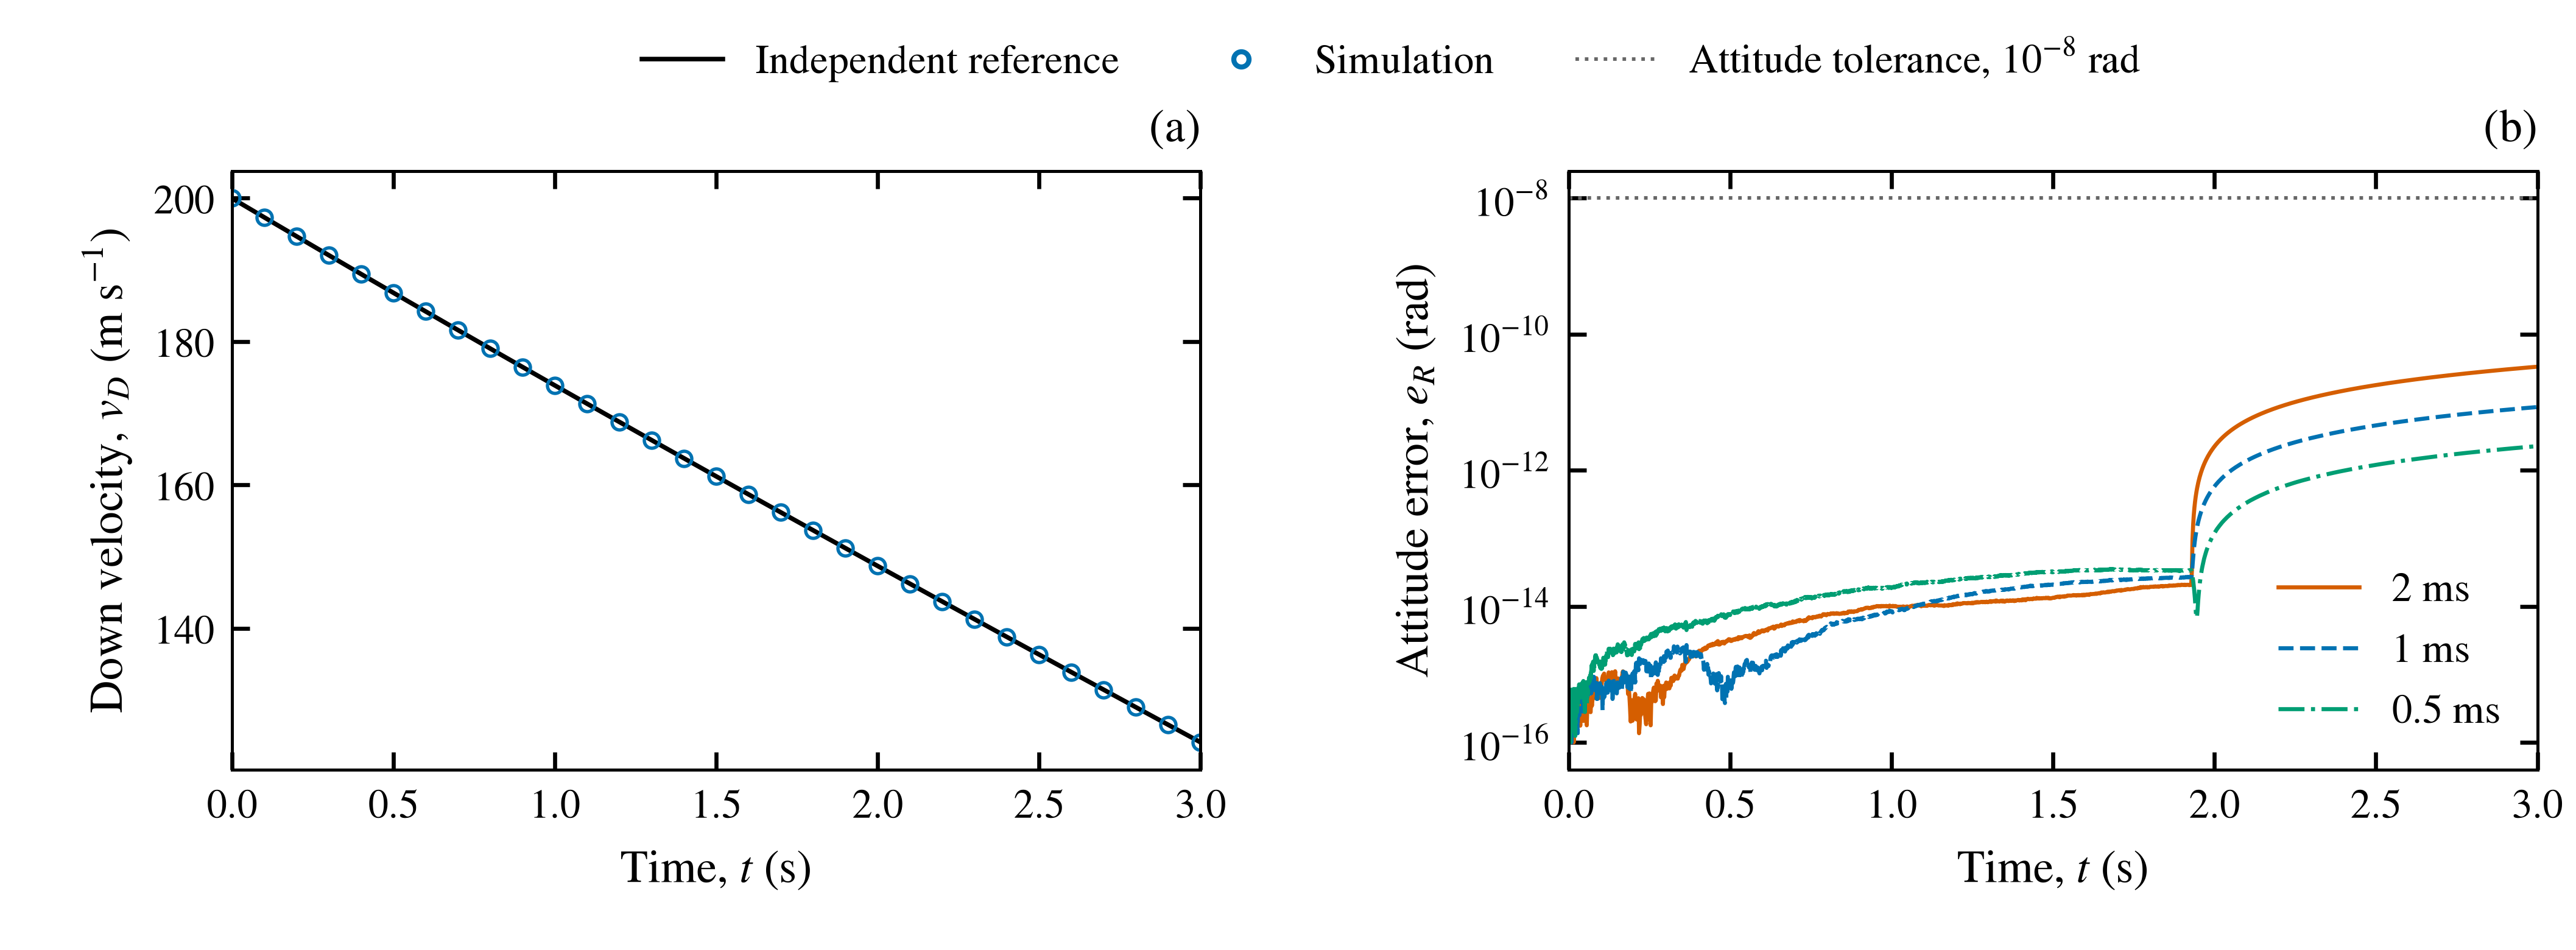
\includegraphics[width=\textwidth]{images/physics_coupled_6dof.png}
  \caption{Coupled six-degree-of-freedom verification case: simulation samples agree with the independent reference; attitude errors remain far below the \SI{1e-8}{\radian} tolerance. Source: supplied verification report~\cite{physics_report}.}
  \label{fig:coupled-verification}
\end{figure}

The entry-burn threshold exceedance and the local QOCO compatibility failure remain open verification limitations. The former is a small but formal failure of the configured mass-refinement criterion; the latter means the local full test suite is not reported as passing. Neither is hidden by the passing checks above.

\subsection{Synthetic Navigation Comparison}

The fixed-truth analysis was run with \sourcecode{python scripts/analyze\_navigation.py scenario=project2\_landing}, using 3,494 navigation epochs over the simulated landing trajectory. The online controller in this analysis uses identity navigation to create the truth trajectory; the sensor packets and both navigation estimates are then generated on that same trajectory with shared initial position, velocity, attitude, and mass. This isolates estimator behavior from closed-loop trajectory changes. The RMSE values in Table~\ref{tab:nav-rmse} are against simulator truth and must not be interpreted as measured CRS-11 errors.

\begin{table}[H]
\centering
\caption{Same-truth IMU-only INS and aided ESKF comparison for the seeded Project~2 landing trajectory.}\label{tab:nav-rmse}
\begin{tabular}{lrrr}
\toprule
\rowcolor{navy}\color{white}\textbf{Error quantity} & \color{white}\textbf{INS-only RMSE} & \color{white}\textbf{ESKF RMSE} & \color{white}\textbf{Effect of aiding}\\
\midrule
Position & \SI{3.450}{\metre} & \SI{0.373}{\metre} & Lower\\
\rowcolor{lightblue}
Velocity & \SI{0.525}{\metre\per\second} & \SI{0.0875}{\metre\per\second} & Lower\\
Attitude rotation error & \SI{0.00139}{\radian} & \SI{0.00483}{\radian} & Higher\\
\rowcolor{lightblue}
Body angular-rate error & \SI{7.73e-4}{\radian\per\second} & \SI{8.20e-4}{\radian\per\second} & Slightly higher\\
\bottomrule
\end{tabular}
\end{table}

The 8--12~s outage removed all 41 scheduled GNSS samples in that interval; two additional scheduled samples were lost to the configured random-dropout process. One gross GNSS outlier was injected at 4~s and rejected by the innovation gate. Across the trajectory, 131 of 132 available GNSS updates and 346 of 350 radar updates were accepted. The mean accepted normalized innovation squared (NIS) was 6.27 for the six-dimensional GNSS update and 1.01 for the scalar radar update. The mean nine-state NEES was 3.10, below its nominal nine-degree-of-freedom expectation; 52.6\% of epochs fell within the nominal pointwise 95\% NEES bounds, and observed component-wise position, velocity, and attitude 3$\sigma$ coverage was 100\%. The estimated gyro- and accelerometer-bias RMSEs were \SI{3.10e-4}{\radian\per\second} and \SI{0.0384}{\metre\per\second\squared}, respectively. These diagnostics suggest a conservative, uncalibrated covariance model. Because errors are temporally correlated and the mechanization is approximate, the nominal per-sample NEES bounds are descriptive rather than an independent-trial consistency test.

The full comparison records truth/estimate histories, sensor packets, covariance, innovations, and metrics in \sourcecode{navigation\_comparison.npz} and \sourcecode{navigation\_comparison.json}. The flight-path overlay, state history, error/3$\sigma$ plot, and innovation/bias plot are reproduced in Appendix~\ref{app:navplots}. Selecting \sourcecode{gnc/navigation=synthetic\_eskf} in \sourcecode{run\_single.py} also generates these comparison files in that run's output folder; the normal Project~2 landing run continues to use identity navigation unless explicitly overridden.

\section{Comparison with CRS-11 Webcast Reconstruction}\label{sec:comparison}

The supplied CRS-11 reconstruction is useful as an observable-flight reference and as a source of nominal scale for initial conditions. For example, the entry-burn, aerodynamic-descent, and powered-descent initial heights and speeds in the Project~2 scenarios correspond closely to the reconstructed event conditions. It is not a complete six-degree-of-freedom ground-truth data set: the broadcast-derived observables do not separate vehicle state, sensor error, data-processing error, altitude datum, or reference-frame convention. The code documentation therefore treats flight comparison as an explicit opt-in analysis rather than a physics acceptance criterion~\cite{scenario_spec,physics_report}.

The archive's opt-in comparator was executed against the supplied reconstruction. It aligns each scenario with the corresponding reference segment and reports altitude and speed residuals over the overlapping interval. Table~\ref{tab:flight-rmse} gives the resulting error statistics. The short entry-burn comparison has the smallest residuals; this is expected because its initial condition and duration closely correspond to the available reference segment. The ascent discrepancy is much larger because its prescribed-input experiment is not calibrated to the webcast mission. The powered-descent overlap ends early because the experiment lasts \SI{22}{\second}, while the available reconstructed reference segment is longer. The comparison plots are included in Appendix~\ref{app:comparisonplots}.

\begin{table}[H]
\centering
\footnotesize
\begin{tabularx}{\textwidth}{@{}p{0.18\textwidth}*{5}{>{\centering\arraybackslash}X}@{}}
\toprule
\rowcolor{navy}\color{white}\textbf{Case} & \color{white}\textbf{Overlap [s]} & \color{white}\textbf{Altitude bias [m]} & \color{white}\textbf{Altitude RMSE [m]} & \color{white}\textbf{Speed bias [m/s]} & \color{white}\textbf{Speed RMSE [m/s]}\\
\midrule
Ascent & 143.643 & 7364.973 & 10721.563 & 160.777 & 203.029\\
\rowcolor{lightblue}
Entry burn & 11.979 & -103.263 & 135.052 & -11.414 & 22.149\\
Aerodynamic descent & 44.979 & 250.098 & 650.004 & 43.290 & 59.871\\
\rowcolor{lightblue}
Powered descent & 21.955 & 502.968 & 617.790 & -53.588 & 56.141\\
\bottomrule
\end{tabularx}
\caption{Observable comparison to the CRS-11 reconstruction from the executed opt-in comparator. These are not navigation errors or physics-acceptance metrics.}\label{tab:flight-rmse}
\end{table}

\begin{table}[H]
\centering
\small
\begin{tabularx}{\textwidth}{Yrrrr}
\toprule
\rowcolor{navy}\color{white}\textbf{Event} & \color{white}\textbf{T+ [s]} & \color{white}\textbf{Altitude [km]} & \color{white}\textbf{Speed [m/s]} & \color{white}\textbf{Downrange [km]}\\
\midrule
Max-Q & 65 & 8.77 & 310 & 1.24\\
\rowcolor{lightblue}
MECO & 145 & 62.36 & 1684 & 43.34\\
Boostback ignition & 161 & 79.23 & 1579 & 63.18\\
\rowcolor{lightblue}
Boostback cutoff & 211 & 113.53 & 588 & 87.92\\
Apogee & 248 & 120.12 & 475 & 70.43\\
\rowcolor{lightblue}
Entry burn ignition & 372 & 47.46 & 1260 & 10.78\\
Entry burn cutoff & 384 & 35.01 & 954 & 5.90\\
\rowcolor{lightblue}
Landing burn ignition & 429 & 4.74 & 320 & -5.37\\
Landing burn cutoff & 462 & $\approx 0$ & 4.3 & -6.53\\
\bottomrule
\end{tabularx}
\caption{CRS-11 reconstructed event states supplied by the team.}\label{tab:crs-events}
\end{table}

\begin{table}[H]
\centering
\small
\begin{tabularx}{\textwidth}{Yrr}
\toprule
\rowcolor{navy}\color{white}\textbf{Event} & \color{white}\textbf{Vertical velocity [m/s]} & \color{white}\textbf{Horizontal velocity [m/s]}\\
\midrule
Max-Q & 305 & 59\\
\rowcolor{lightblue}
MECO & 1155 & 1229\\
Boostback ignition & 992 & 1229\\
\rowcolor{lightblue}
Boostback cutoff & 360 & -465\\
Apogee & 0 & -475\\
\rowcolor{lightblue}
Entry burn ignition & -1248 & -182\\
Entry burn cutoff & -932 & -204\\
\rowcolor{lightblue}
Landing burn ignition & -319 & -32\\
Landing burn cutoff & -4.3 & 0\\
\bottomrule
\end{tabularx}
\caption{CRS-11 reconstructed velocity components. Signs are reproduced as provided; the exact coordinate convention remains uncertain.}\label{tab:crs-components}
\end{table}

The Project~2 ascent case should not be judged by direct agreement with the MECO row: it uses assumed throttle, gimbal, atmospheric, mass, and reference-site conditions and ends at \SI{101.056}{\kilo\metre} and \SI{2171.271}{\metre\per\second} after \SI{150}{\second}, whereas the webcast reconstruction gives approximately \SI{62.36}{\kilo\metre} and \SI{1684}{\metre\per\second} at MECO. That difference is expected in an independent physics experiment. By contrast, the aerodynamic-descent case begins at the reconstructed entry-burn-cutoff scale and ends after \SI{45}{\second} at \SI{3.758}{\kilo\metre} and \SI{310.462}{\metre\per\second}, close in scale to the reconstructed landing-burn-ignition values of \SI{4.74}{\kilo\metre} and \SI{320}{\metre\per\second}. This is an engineering consistency observation, not a calibration result.

The residuals in Table~\ref{tab:flight-rmse} use the archive's comparison conventions and are preserved as an observable comparison only. No parameters were calibrated to minimise these errors, and no sensor measurement was used. Therefore the table is useful for scale and model-context discussion, but it is not a navigation-filter error analysis.

\section{Navigation Performance}\label{sec:navigation-performance}
% Shared by main.tex and report.tex; numerical tables are generated from executed runs.
\subsection{Experiment Design and Error Definitions}\label{sec:nav-experiments}

The navigation campaign was executed on 10 November 2026 using
\path{report_assets/generate_navigation.py}, with the physically sampled ESKF and
seed~0 for the paired comparisons, supplemented by the multi-seed experiments below. It supplements the earlier physics campaign. Two paired closed-loop tests use
\path{project2_landing} and \path{flight_calibrated_landing}. Within each pair,
the resolved configuration is identical except for the navigation module; the generation
script checks that invariant. Initial-state dispersion is disabled. Each run propagates
its own closed-loop trajectory, so the comparison measures the effect of navigation on
the combined estimation, planning, and control response.

The Project~2 pair starts at 300 m and 25 m/s downward speed, with ideal actuators and a
free-terminal-time LCvx plan. The calibrated pair starts at 348.764 m and 76.111 m/s
downward speed, with mass 35,692.161 kg, realistic actuators, and the scenario's previously
selected aerodynamic parameters. Its LCvx plan uses a 12.145 s terminal time, a 30 kN/s
planned thrust-rate limit, and vertical tracking gains of 6 s$^{-2}$ and 4 s$^{-1}$.
These settings originate from the separate flight-calibration study; no parameters are
refitted to the sensor samples. Neither differences between these two scenario families
nor the calibrated scenario's fit to public observables are treated as navigation errors.
Both use a 1 ms plant step, 10 ms navigation period, and 20 ms control period. The guidance
interface is called every second, but \texttt{convex\_replan=false} retains the initial plan
while tracking feedback continues. Trajectory logging periods remain 100 ms and 20 ms,
respectively; all navigation errors use the full 10 ms navigation grid.

For vector state $\bm x$, error magnitude and reported summary statistics are
\begin{equation}
 e_k=\|\widehat{\bm x}_k-\bm x_{truth,k}\|_2,\qquad
 \mathrm{RMSE}=\sqrt{\frac1N\sum_{k=1}^{N}e_k^2},\qquad e_{\max}=\max_k e_k.
\end{equation}
Attitude error is the shortest relative-quaternion rotation angle, reported in degrees;
angular-rate error is the norm of the body/reference rate difference, reported in degrees
per second. Initialization transients are included. Navigation samples stop at the last
scheduled update before the plant terminates. Ground-contact speed, miss distance, and
tilt use the simulator's interpolation to zero radial altitude; contact time in the tables
is interpolated with the same logged-state bracket. These terminal quantities and the
navigation samples are therefore evaluated at distinct epochs.

\subsection{Closed-Loop Navigation and Landing Results}\label{sec:nav-closed-loop}

All four nominal cases reach a soft landing under the existing simulator criteria.
Table~\ref{tab:nav-contact} compares the paired terminal results and
Table~\ref{tab:nav-errors} reports ESKF accuracy against each run's own truth.
Identity navigation has exactly zero estimation error because it returns truth.
It is an ideal-feedback reference, not an unfiltered sensor estimator.

\begin{table}[!htbp]\centering\small
\caption{Paired closed-loop results, seed 0. Each pair changes only navigation.
All four cases satisfy the simulator's soft-landing and success criteria.}\label{tab:nav-contact}
% Generated by report_assets/generate_navigation.py; do not edit numbers.
\begin{tabularx}{\textwidth}{ll*{4}{>{\raggedleft\arraybackslash}X}}\toprule
Scenario & Navigation & Contact [s] & Speed [m/s] & Miss [m] & Tilt [deg]\\\midrule
Project 2 & Identity & 17.468 & 0.086 & 0.019 & 0.055\\
Project 2 & ESKF & 17.583 & 1.381 & 0.788 & 0.219\\
Calibrated & Identity & 12.230 & 0.483 & 0.014 & 0.062\\
Calibrated & ESKF & 12.195 & 0.553 & 0.602 & 1.097\\
\bottomrule\end{tabularx}

\end{table}

\begin{table}[!htbp]\centering\small
\caption{ESKF navigation error statistics on the full navigation grid. Vector entries use
norms, not componentwise averages.}\label{tab:nav-errors}
\begin{tabularx}{\textwidth}{ll*{4}{>{\raggedleft\arraybackslash}X}}\toprule
Scenario & Statistic & Position [m] & Velocity [m/s] & Attitude [deg] & Rate [deg/s]\\\midrule
Project 2 & RMSE & 0.540 & 0.066 & 1.356 & 0.048\\
Project 2 & MAX & 2.879 & 0.182 & 2.444 & 0.131\\
Calibrated & RMSE & 0.641 & 0.074 & 1.189 & 0.049\\
Calibrated & MAX & 2.879 & 0.166 & 2.282 & 0.125\\
\bottomrule\end{tabularx}

\end{table}
\FloatBarrier

The ESKF introduces observable feedback consequences. In the Project~2 pair, contact speed
increases from 0.086 to 1.381 m/s while the position-estimation RMSE is 0.540 m. In the
calibrated pair, contact speed changes from 0.483 to 0.553 m/s and horizontal miss increases
from 0.014 to 0.602 m, with position-estimation RMSE 0.641 m. Thus sub-metre average
estimation error does not imply unchanged terminal performance. The plots show estimation
transients and the resulting trajectories; they do not establish robustness probabilities
from a single noise realization.

\begin{figure}[!htbp]\centering
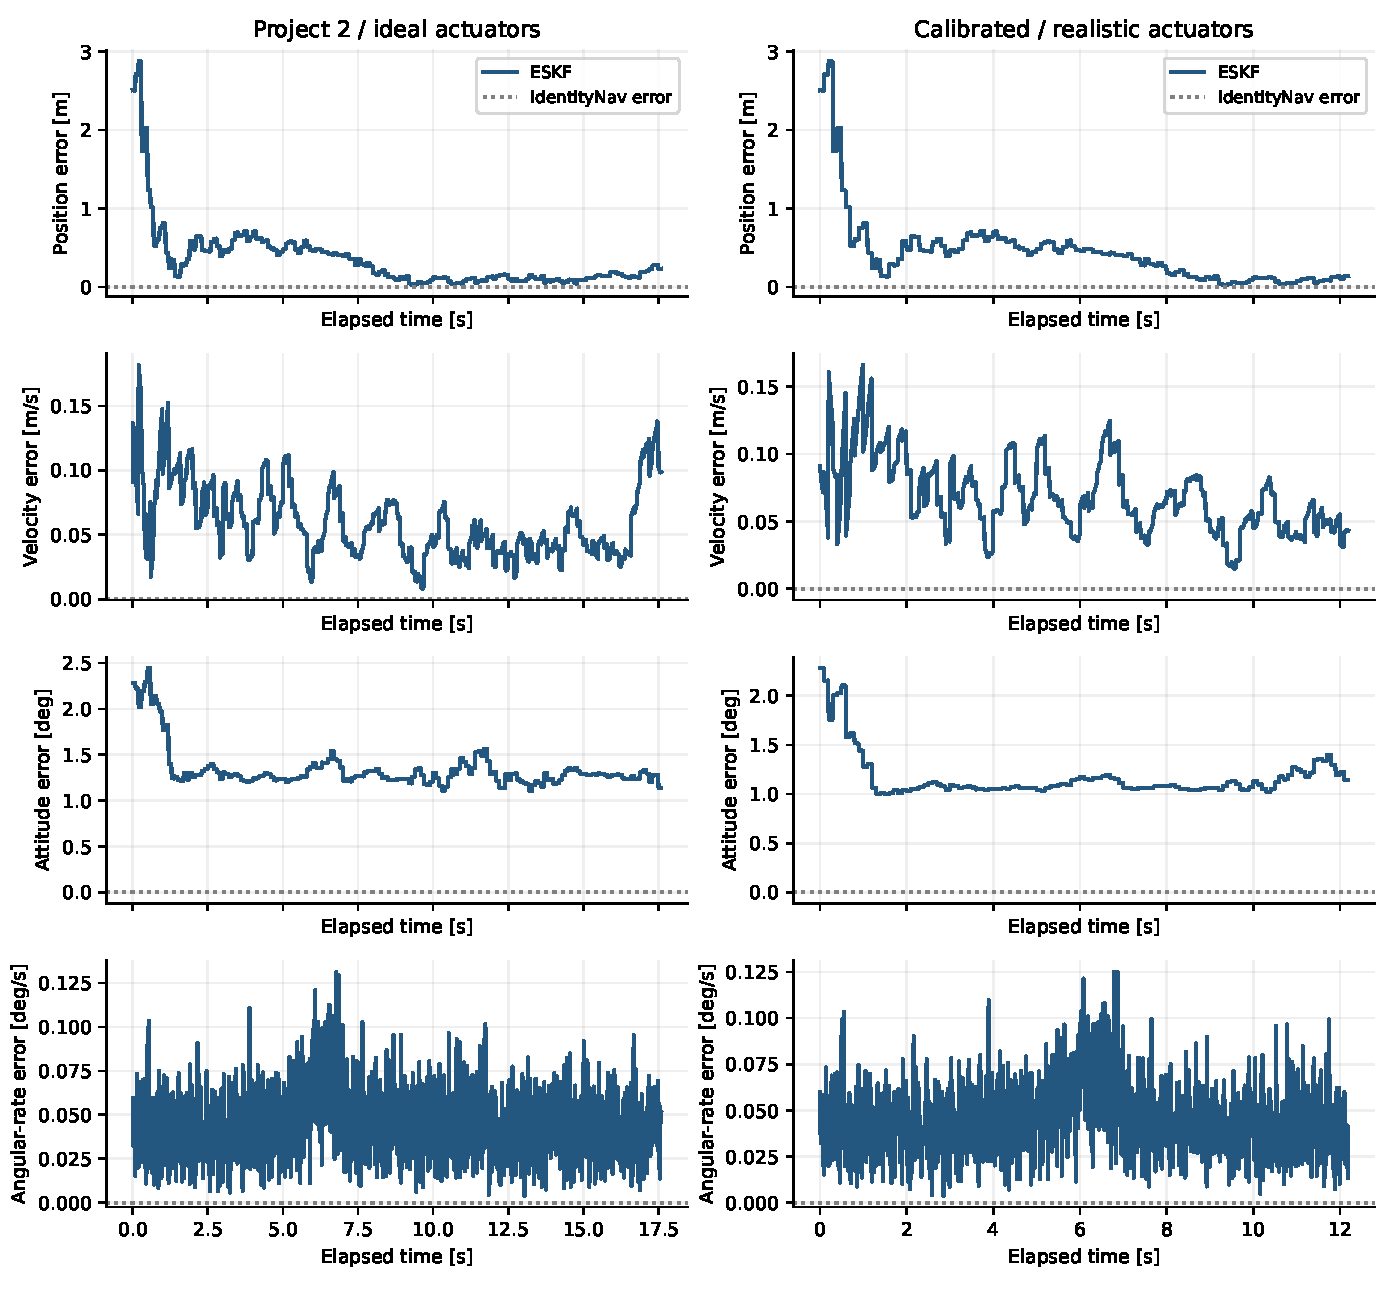
\includegraphics[width=\textwidth,height=0.72\textheight,keepaspectratio]{report_assets/navigation_closed_loop.pdf}
\caption{ESKF position, velocity, attitude, and angular-rate error norms in the two
closed-loop cases. Dotted zero lines indicate ideal-feedback estimation error.
Each ESKF history is compared with its own plant truth.}\label{fig:nav-closed-loop}
\end{figure}

\begin{figure}[!htbp]\centering
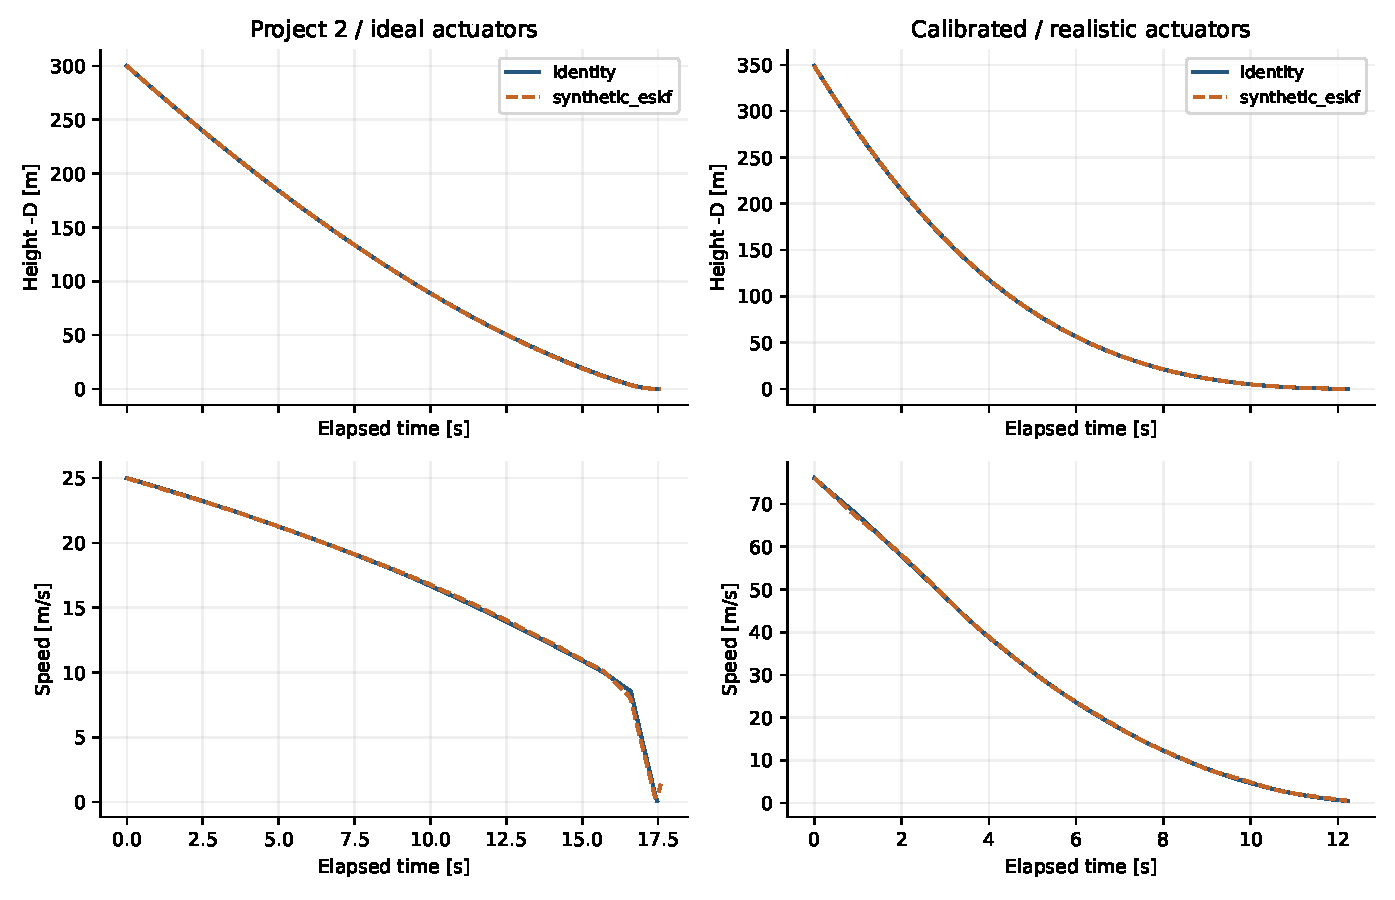
\includegraphics[width=\textwidth,height=0.58\textheight,keepaspectratio]{report_assets/navigation_landing.pdf}
\caption{True height and speed under identity and ESKF feedback. The height curves use
the near-pad tangent height $-r_D$; contact metrics use radial altitude.
Each panel retains its scenario's plant and controller settings.}\label{fig:nav-landing}
\end{figure}

\subsection{Fixed-Trajectory Filter Comparison and GNSS Outage}\label{sec:nav-replay}

To isolate estimation from changing closed-loop trajectories, the calibrated identity
run's truth is replayed at 100 Hz. Native CG force and inertial-rate histories are recorded at every navigation epoch.
One sensor generator uses these histories to create a common sample sequence; each filter receives an independent copy of the same measurements. Three cases
share the same GNSS/radar initialization and uncertain alignment observation: IMU-only propagation
with all subsequent aiding disabled, the nominal ESKF, and an ESKF with GNSS updates
suppressed from 4 through 8 s while radar remains available. The replay has 1,223 IMU
samples over 0--12.22 s, 121 valid nominal GNSS updates, and 245 radar samples. Suppressing
the selected interval leaves 80 GNSS updates. No replay estimate is fed back into the plant.

\begin{table}[!htbp]\centering\small
\caption{RMSE on identical truth and sensor samples. The IMU-only case retains the common
initial aided update and then propagates without further GNSS or radar corrections.}
\label{tab:nav-replay}
\begin{tabularx}{\textwidth}{l*{4}{>{\raggedleft\arraybackslash}X}}\toprule
Replay case & Position [m] & Velocity [m/s] & Attitude [deg] & Rate [deg/s]\\\midrule
IMU only & 19.732 & 4.307 & 2.318 & 0.044\\
ESKF & 0.641 & 0.075 & 1.091 & 0.049\\
ESKF + GNSS outage & 0.756 & 0.068 & 1.114 & 0.045\\
\bottomrule\end{tabularx}

\end{table}
\FloatBarrier

GNSS/radar aiding reduces position RMSE from 19.732 to 0.641 m and velocity RMSE from
4.307 to 0.075 m/s. A four-second GNSS outage increases position RMSE to 0.756 m; radar
continues to constrain height. The slight decrease in aggregate velocity RMSE during this
particular outage is not evidence that discarding GNSS is beneficial. It is one finite
noise realization, and the horizontal and vertical channels have different aiding.

With uncertain initial alignment, attitude RMSE decreases from 2.318 deg in IMU-only
propagation to 1.091 deg with ESKF aiding. Angular-rate RMSE is 0.044 deg/s and
0.049 deg/s, respectively: aiding does not reduce every error metric. The short,
nearly vertical trajectory has no direct attitude observation after initialization.
Figure~\ref{fig:nav-biases} shows that not every bias component converges; the longer
ascent and consistency experiments below examine a wider excitation and time range.

\begin{figure}[!htbp]\centering
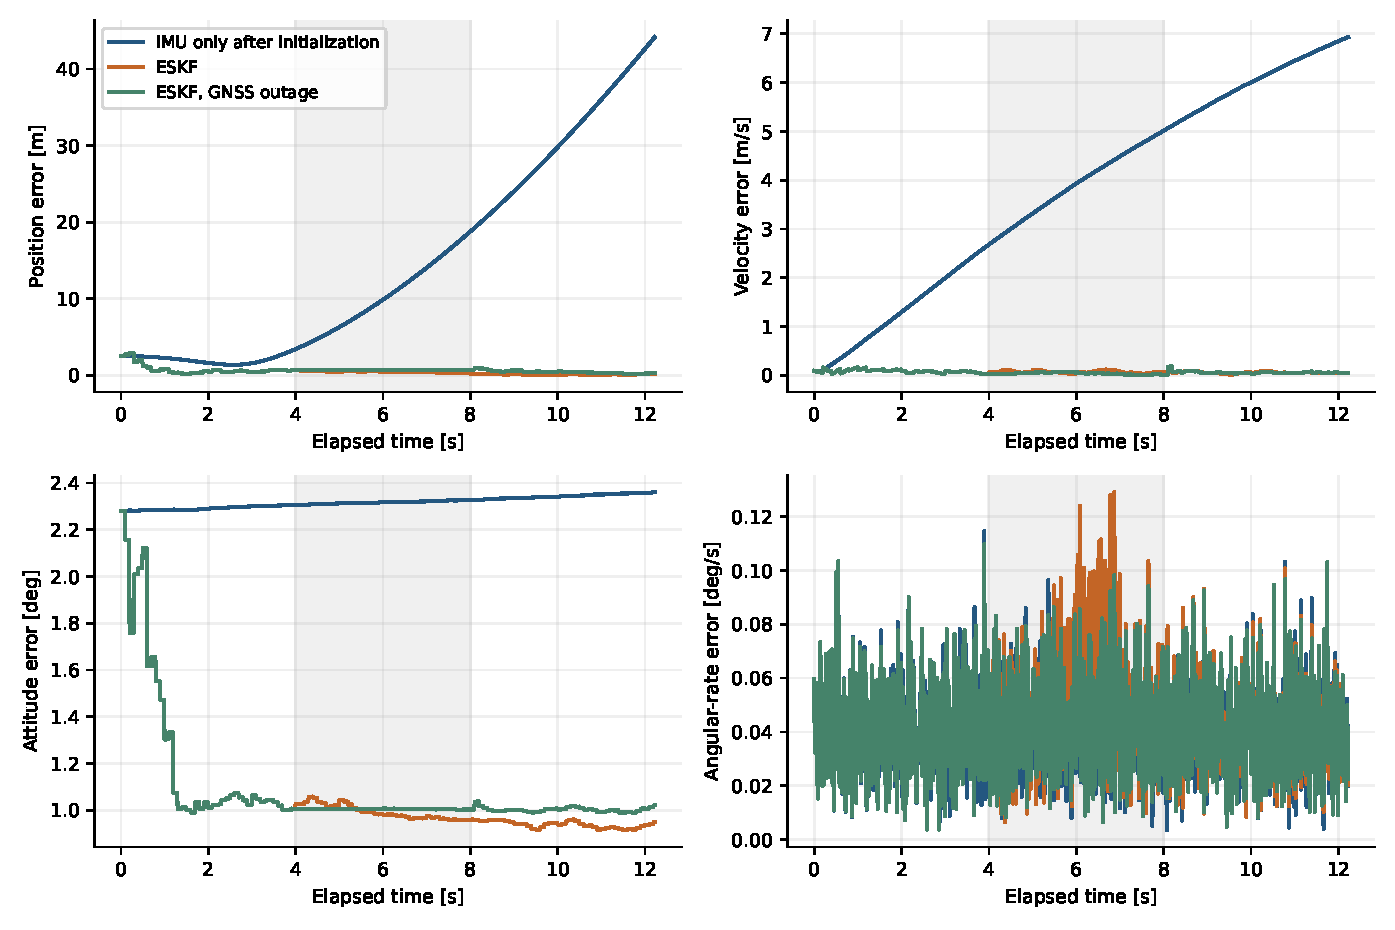
\includegraphics[width=\textwidth,height=0.60\textheight,keepaspectratio]{report_assets/navigation_replay.pdf}
\caption{Fixed-truth replay comparison. The shaded interval is the GNSS outage applied
only to the outage variant; radar remains active. All three cases receive the same IMU
samples and start from the same nominal state and covariance.}\label{fig:nav-replay}
\end{figure}

\begin{figure}[!htbp]\centering
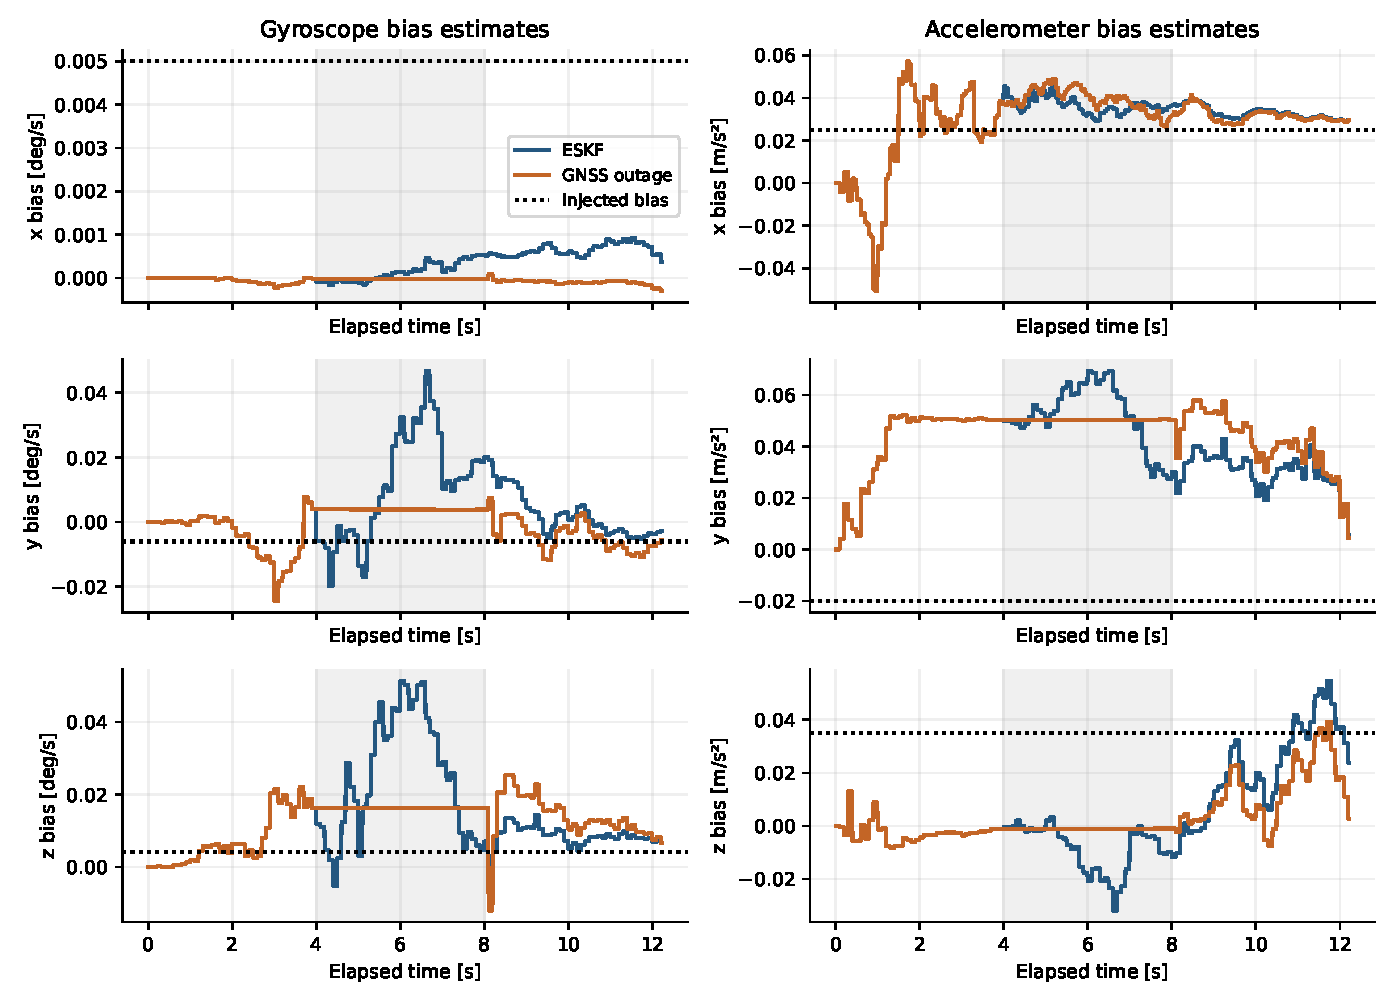
\includegraphics[width=\textwidth,height=0.63\textheight,keepaspectratio]{report_assets/navigation_biases.pdf}
\caption{Estimated IMU biases in fixed-truth replay, with the constant injected biases
shown as dotted lines. The short experiment does not show convergence of every bias
component. The shaded interval suppresses GNSS only in the outage variant.}\label{fig:nav-biases}
\end{figure}

\FloatBarrier
\subsection{Multiple Seeds and Missing-GNSS Startup}\label{sec:nav-robustness}
Each landing scenario is repeated with seeds 0--9, a 1 deg per-axis initial alignment
uncertainty, and the same sensor parameters and unchanged controller settings. A third
condition uses the Project~2 landing with GNSS suppressed from 0 through 3 s. Its declared
initial position prior has offset $(10,-8,5)$ m and velocity prior has offset
$(0.5,-0.4,0.3)$ m/s; radar remains available. Thus the prior is deliberately different
from truth, and the estimator must propagate and acquire GNSS after startup.
\begin{table}[!htbp]\centering\small
\caption{Ten-seed closed-loop evaluation per condition. Maxima include unsuccessful runs;
mean position RMSE is the arithmetic mean of the ten per-run RMSEs.}\label{tab:nav-seeds}
\begin{tabularx}{\textwidth}{Yrrrr}\toprule
Case & Soft success & Max speed [m/s] & Max miss [m] & Mean pos. RMSE [m]\\\midrule
Project 2 & 5/10 & 6.539 & 1.152 & 0.539\\
Calibrated & 10/10 & 1.314 & 1.836 & 0.615\\
Project 2, startup outage & 4/10 & 4.444 & 4.358 & 5.973\\
\bottomrule\end{tabularx}

\end{table}
\FloatBarrier
The calibrated realistic-actuator case succeeds in all ten runs. The original Project~2
configuration succeeds in five; with the startup outage and perturbed prior it succeeds
in four. The nominal Project~2 maximum contact speed is 6.539 m/s despite a mean
position-estimation RMSE of 0.539 m. These outcomes show that the original ideal-actuator
landing configuration is sensitive to state-estimation errors. Successful initialization
and sub-metre average estimation error do not guarantee a soft landing. The empirical
counts describe these finite trials, not a qualified flight success probability; no
controller gains were changed to improve the counts. The two scenario families differ in
initial condition, vehicle and guidance settings, so their success counts do not isolate
the effect of actuator fidelity.

\subsection{Long Ascent Replay and Covariance Diagnostics}\label{sec:nav-consistency}
The native 150-second \texttt{project2\_ascent} trajectory is recorded at 100 Hz,
including its 10--12 s gimbal maneuver, throttle changes, cutoff at 145 s, and coast.
The physical IMU channels come directly from native loads and inertial angular rates.
Five seeds (0--4) are replayed under three conditions: nominal aiding, no GNSS from
0 through 5 s, and no GNSS from 60 through 80 s. The startup case uses the same nonzero
prior offsets as the landing test. All variants within each seed receive identical
sensor samples and alignment observation; only GNSS availability and the startup
initialization differ. Radar follows the 1500 m range limit and cannot aid the
high-altitude 20-second outage. Estimates are not fed back into this prescribed ascent.
\begin{table}[!htbp]\centering\small
\caption{Five-seed 150-second ascent replay. RMSE columns are means of per-run RMSEs;
NEES is averaged over the five seeds and all sampled epochs.}\label{tab:nav-ascent}
\begin{tabularx}{\textwidth}{Yrrrr}\toprule
Ascent case & Pos. RMSE [m] & Vel. RMSE [m/s] & Att. RMSE [deg] & Mean NEES\\\midrule
Nominal & 0.380 & 0.054 & 0.750 & 10.70\\
Startup outage (5 s) & 2.833 & 0.262 & 0.866 & 10.83\\
In-flight outage (20 s) & 1.059 & 0.143 & 0.933 & 11.17\\
\bottomrule\end{tabularx}

\end{table}
\FloatBarrier
All startup-outage runs acquire GNSS at 5.1 s. Initial attitude-error magnitudes range
from 0.703 to 2.332 deg. Across the fifteen ascent replays, final position-error magnitude
is at most 0.414 m and final attitude error at most 0.715 deg. The nominal mean position
RMSE is 0.380 m; the startup and in-flight outages increase it to 2.833 and 1.059 m.
The maximum transient position errors are 23.389 m and 8.664 m in the two outage
conditions. These results demonstrate recovery after aiding returns, rather than
continuous nominal accuracy during the outages.

The full 15-state normalized estimation error squared and measurement normalized
innovation squared are
\begin{equation}
 \mathrm{NEES}_k=\bm e_k^TP_k^{-1}\bm e_k,\qquad
 \mathrm{NIS}_k=\bm y_k^TS_k^{-1}\bm y_k,
\end{equation}
where $\bm e$ includes position, velocity, global attitude error, and both bias errors.
For five independent seeds, the reference pointwise 95\% band for mean NEES is
$[10.588,20.168]$, obtained from a chi-square distribution with 75 degrees of freedom.
Mean GNSS NIS is 5.995--6.007 (six measurement components), and mean altimeter NIS is
0.992--0.997 (one component). However, only 50.4--59.0\% of epochs have ensemble NEES
inside the reference band. Thus measurement innovations have appropriate mean scale
in these tests, while full-state covariance consistency is not established. The fixed
injected biases are not sampled from the complete Gaussian prior, process bias noise
allows variation absent from truth, and temporal samples are correlated. The band is a
diagnostic reference, not a sequence of independent acceptance tests or a reason to
retune covariance until a desired pass fraction is obtained.
\begin{figure}[!htbp]\centering
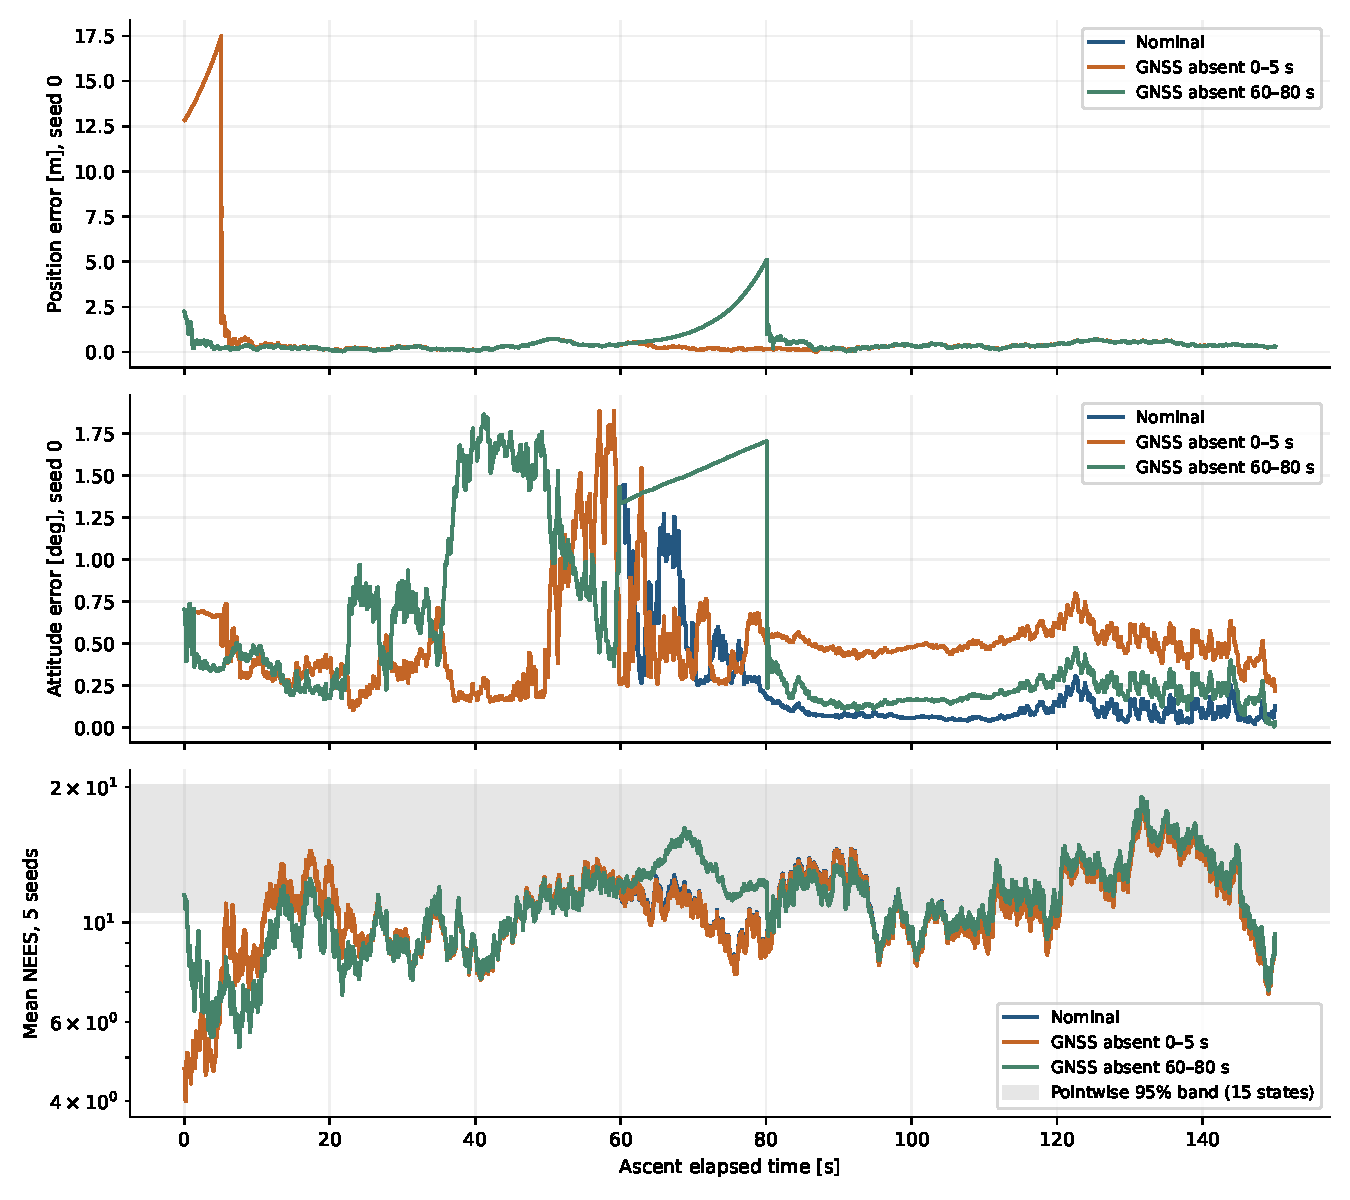
\includegraphics[width=\textwidth,height=0.72\textheight,keepaspectratio]{report_assets/navigation_robustness.pdf}
\caption{Native ascent replay: seed-0 position and attitude error, and five-seed mean NEES.
The pointwise consistency band is shown for the 15-state error.}\label{fig:nav-robustness}
\end{figure}
\FloatBarrier

\subsection{Verification Scope and Remaining Navigation Limitations}\label{sec:nav-limits}
Physical checks cover zero accelerometer output in vacuum free fall, pad support,
Earth-rate gyro output, and drift-free noiseless propagation at an Earth-fixed point
away from the reference origin. Finite differences verify the radial-height/gravity
Jacobians and global attitude reset. Initialization tests exercise absent GNSS,
nonzero alignment error, and single use of the first GNSS sample. Replay checks include
finite estimates, quaternion normalization, and covariance positivity. Additional checks
verify optional scale-factor/random-walk inputs, explicit sensor-rate validation, GNSS
outlier rejection, and common uncertain initialization of the IMU-only and aided estimators.

The expanded study evaluates small unknown alignment errors, delayed GNSS acquisition,
multiple seeds, and longer high-altitude outages. It does not establish autonomous
alignment from an arbitrary unknown attitude, hardware sensor accuracy, global
covariance consistency, or robust landing over the full operating envelope. Mass remains
an ideal auxiliary measurement. The sensors omit latency, lever arms, saturation, and
vibration; the altimeter assumes radial height. These technical limits remain relevant
to guidance and control design even when the filter is numerically well behaved.


\section{Assumptions, Limitations, and GNC Risks}\label{sec:assumptions}

The Project~2 briefing requires a clear separation of known, estimated, and assumed information. Table~\ref{tab:assumptions} provides a concise ledger for the current implementation. Keeping this distinction explicit is essential because numerical verification demonstrates correct implementation of declared equations, not empirical agreement with an operational vehicle.

\begin{table}[H]
\centering
\begin{tabularx}{\textwidth}{p{0.19\textwidth}YY}
\toprule
\rowcolor{navy}\color{white}\textbf{Category} & \color{white}\textbf{Examples in the present work} & \color{white}\textbf{Consequence for interpretation}\\
\midrule
Known / code-defined & Equations, numerical scheme, scheduled inputs, code configuration, output conventions & Can be reproduced and numerically verified\\
\rowcolor{lightblue}
Estimated from webcast context & Representative entry, descent, and landing-burn altitude/speed scales & Useful for initial-condition selection; uncertain as flight truth\\
Engineering assumptions & Masses, tank geometry, \SI{914}{\kilo\newton} engine model, aero coefficients, \ang{28.6} latitude, no wind/fault/slosh & Must be sensitivity-tested before design decisions\\
\rowcolor{lightblue}
Not modeled / incomplete & Calibrated sensors, rotating-Earth INS mechanization, online filter calibration, realistic-actuator landing qualification, leg impact, J2/oblateness, validated flight aerodynamics & Cannot support a claim of operational GNC readiness\\
\bottomrule
\end{tabularx}
\caption{Assumption and evidence ledger.}\label{tab:assumptions}
\end{table}

\subsection{Most Dangerous Errors for Future Guidance and Control}

\begin{longtable}{p{0.22\textwidth}p{0.42\textwidth}p{0.24\textwidth}}
\toprule
\rowcolor{navy}\color{white}\textbf{Potential error} & \color{white}\textbf{Why it is dangerous} & \color{white}\textbf{Recommended mitigation}\\
\midrule
\endfirsthead
\toprule
\rowcolor{navy}\color{white}\textbf{Potential error} & \color{white}\textbf{Why it is dangerous} & \color{white}\textbf{Recommended mitigation}\\
\midrule
\endhead
Navigation state or bias error & Guidance may solve the correct problem from the wrong position, velocity, attitude, or mass state; terminal constraints can be missed even with a feasible plan. & Calibrate the synthetic model; test online closed-loop behavior under bias, dropout, delay, and uncertainty.\\
\rowcolor{lightblue}
Thrust magnitude or throttle-lag error & Landing fuel margin and burn timing are highly sensitive to effective thrust. Ideal actuation can mask a late or underperforming engine response. & Run dispersions with realistic actuator dynamics, thrust bias, minimum throttle, and engine-out cases.\\
Aerodynamic coefficient or wind error & During entry and grid-fin descent, force/moment errors create trajectory, attitude, and load errors that propagate into landing initialization. & Use bounded aerodynamic/wind dispersions and verify controller margins across Mach, alpha, and $\bar q$.\\
\rowcolor{lightblue}
Mass, CG, or inertia error & Allocation and attitude dynamics use moment arms and inertia. Incorrect tank fill or CG produces incorrect gimbal/fin authority. & Calibrate mass properties; sweep propellant, CG, and inertia uncertainty.\\
Reference-frame or Earth-model inconsistency & Mixing Earth-relative and inertial rates or altitude definitions can inject persistent guidance and sensor-model errors. & Maintain explicit frame metadata; cross-check against independent inertial propagation.\\
\rowcolor{lightblue}
Overinterpreted webcast comparison & A small plot mismatch could reflect ambiguous data extraction instead of model error; fitting it can conceal structural errors. & Separate physics verification from observable comparison and report data limitations.\\
\bottomrule
\caption{Risk assessment answering the Project~2 final evaluation question.}\label{tab:risks}
\end{longtable}

\section{Reproducibility and Run Commands}\label{sec:reproducibility}

The baseline physics commands below are adapted from the supplied README and Project~2 specification. They were executed for the original physics campaign using the supplied archive with SHA-256 prefix \texttt{d6022aa6}. The navigation extension uses the current source and the separate provenance record in Section~\ref{sec:nav-reproduction}. Run them from the repository root after creating the required Python environment. The project declares Python~3.10+ and a C++ compiler as prerequisites. Keep each output directory, resolved configuration, manifest, and source revision with the report figures.

\subsection{Installation and Baseline Checks}
\begin{lstlisting}
python -m pip install -e ".[dev,qoco]"
python -m pytest tests/ -q
ruff check src tests scripts
\end{lstlisting}

\subsection{Five Project 2 Runs}
\begin{lstlisting}
.venv/bin/python scripts/run_single.py scenario=project2_ascent hydra.run.dir=results/project2_physics/ascent
.venv/bin/python scripts/run_single.py scenario=project2_entry_burn hydra.run.dir=results/project2_physics/entry_burn
.venv/bin/python scripts/run_single.py scenario=project2_aero_descent hydra.run.dir=results/project2_physics/aero_descent
.venv/bin/python scripts/run_single.py scenario=project2_powered_descent hydra.run.dir=results/project2_physics/powered_descent
.venv/bin/python scripts/run_single.py scenario=project2_landing hydra.run.dir=results/project2_physics/landing
.venv/bin/python scripts/check_project2_segments.py
.venv/bin/python scripts/check_rotating_earth.py
\end{lstlisting}

\subsection{Synthetic Navigation Analysis}
\begin{lstlisting}
python scripts/analyze_navigation.py scenario=project2_landing
python scripts/run_single.py scenario=project2_landing gnc/navigation=synthetic_eskf
\end{lstlisting}

The first command creates a fixed identity-navigation truth rollout and then compares the two
estimators against that same truth. The second selects the synthetic ESKF online for the
closed-loop controller; \sourcecode{run\_single.py} automatically writes the same-truth
post-processing comparison into its Hydra result directory. These are distinct experiments and
should be labeled accordingly in any additional result tables.

\subsection{Optional Public Flight Comparison and Replay}
\begin{lstlisting}
.venv/bin/python scripts/run_single.py scenario=project2_entry_burn scenario.reference.enabled=true hydra.run.dir=results/project2_optional/entry_burn
.venv/bin/python scripts/check_project2_segments.py --compare-flight --output results/project2_optional/checks
.venv/bin/python scripts/view_replay.py results/project2_physics/powered_descent
\end{lstlisting}

The optional comparison command must be reported separately from the physics acceptance checks. An RMSE result is an observable comparison under the selected conventions; it is not proof of vehicle fidelity or navigation accuracy. The normal result folders contain trajectory, actuator, navigation, timing, replay, KPI, and resolved-configuration information, depending on scenario and run mode.

The five phase runs, validation results, and opt-in flight-comparison plots in this report were produced with this command sequence. The resolved configurations and numerical histories identify the evaluated experimental conditions.

\subsection{Navigation Campaign Reproduction}\label{sec:nav-reproduction}

The navigation results are newly executed runs, separate from the archived physics
campaign. From the repository root, regenerate the four paired closed-loop cases, the common-truth
replay, thirty additional landing trials, fifteen ascent replays, and the navigation figures/tables with:
\begin{lstlisting}
.venv/bin/python -m pip install -e ".[dev]"
.venv/bin/python report_assets/generate_navigation.py
.venv/bin/python -m pytest tests/test_synthetic_eskf.py tests/sim/test_timing_contract.py tests/sim/test_multirate.py tests/sim/test_flight_calibration.py -q
\end{lstlisting}
The generator writes resolved configurations, seed manifests, full-rate navigation
histories, physics histories, and contact/error summaries under
\path{results/report_navigation/}. The navigation histories include native specific force and inertial rate at the navigation period.
The fixed-truth replay additionally saves the actual
IMU/GNSS/radar samples, all estimator states, bias estimates, and covariance diagonals.
\path{report_assets/navigation_metrics.json} records source SHA-256 hashes, the base Git
revision, numerical package versions, data hashes, and the evaluation conventions. These records identify the evaluated source and environment.
The figures and generated numerical tables in \path{report_assets/navigation_*} are
included in the report source tree; the \path{results/} histories can be regenerated with the same command
or supplied with the results archive to inspect the complete time histories.

For a normal standalone run with replay and sensor post-processing:
\begin{lstlisting}
.venv/bin/python scripts/run_single.py scenario=flight_calibrated_landing gnc/navigation=synthetic_eskf hydra.run.dir=results/navigation_landing
\end{lstlisting}
Replacing \texttt{synthetic\_eskf} with \texttt{identity} selects exact state feedback.
The standalone runner's additional sensor CSVs are generated after the flight; the ESKF
has already used its online sensor model during the closed-loop simulation.

The IMU rate and navigation period are explicit and must agree; the report settings use
100 Hz and 10 ms. Neither runner changes the period automatically. An independent
same-truth comparison and diagnostic plots can also be generated with:
\begin{lstlisting}
.venv/bin/python scripts/analyze_navigation.py scenario=project2_landing
\end{lstlisting}
This optional comparison uses the same physical sensor and rotating-frame propagation.
Its seeded replay is separate from the online samples that influenced a closed-loop run.
Scale-factor, bias-random-walk, outlier and gate settings are optional experiments; the
nominal report configuration keeps them disabled.


\section{Conclusions and Remaining Work}\label{sec:conclusion}

The supplied RLV-Sim archive is a credible Project~2 simulator baseline. Its modular separation of plant, GNC, configuration, and simulation harness makes it suitable for later guidance and control work. It represents the physics needed to produce representative ascent and recovery trajectories rather than only replaying a pre-recorded path. The five phase cases were executed successfully, and demonstrate the intended range from powered ascent through soft landing.

The report should nevertheless remain precise about scope. The code verifies its declared equations and numerical implementation; it does not validate all vehicle parameters against the real Falcon~9. The CRS-11 reconstruction is valuable for context and nominal initial conditions but cannot independently validate full state, sensor, or navigation performance. The synthetic sensor-and-ESKF extension now provides quantified navigation errors and paired closed-loop tests, including realistic actuation. A fixed-truth replay evaluates position, velocity, attitude, and bias estimation. Multi-seed landings and a 150-second ascent replay extend the evaluation to uncertain alignment, missing-GNSS startup, longer outages, and covariance consistency. Remaining priorities are hardware-based sensor parameters, autonomous alignment, covariance calibration, and wider environmental and vehicle dispersions.


\clearpage
\begin{thebibliography}{9}
\bibitem{briefing}
RSLV GNC Project~2, \emph{Development of Vehicle Simulator with Navigation Blocks}. Course briefing slides supplied as PDF.

\bibitem{readme}
RLV-Sim, \sourcecode{README.md}, supplied RLV-Sim-2026-main archive.

\bibitem{architecture}
RLV-Sim, \sourcecode{docs/1\_architecture.md}, supplied RLV-Sim-2026-main archive.

\bibitem{scenario_spec}
RLV-Sim, \sourcecode{docs/reference/project2\_scenario\_spec.md}, supplied RLV-Sim-2026-main archive.

\bibitem{physics_report}
RLV-Sim, \sourcecode{docs/verification/physics\_implementation\_report\_en.md}, supplied RLV-Sim-2026-main archive.

\bibitem{physics_results}
RLV-Sim, \sourcecode{docs/verification/project2\_segments/physics\_results.md}, supplied RLV-Sim-2026-main archive.

\bibitem{configs}
RLV-Sim configuration and source files: \sourcecode{configs/scenario/project2\_*.yaml}, \sourcecode{configs/gnc/*}, \sourcecode{src/sim/*}, \sourcecode{src/gnc/*}, and \sourcecode{src/plant/*}, supplied archive.

\bibitem{nav_implementation}
RLV-Sim navigation comparison implementation: \sourcecode{src/gnc/navigation/synthetic\_eskf.py}, \sourcecode{src/validation/navigation.py}, \sourcecode{scripts/analyze\_navigation.py}, and \sourcecode{scripts/run\_single.py}, supplied archive.

\bibitem{crs11}
CRS-11 reconstructed event data and plots supplied by the team from webcast analysis.
\bibitem{sola} J. Sol\`a, \emph{Quaternion kinematics for the error-state Kalman filter}, 2017. \url{https://arxiv.org/abs/1711.02508}.
\end{thebibliography}

\appendix
\clearpage
\clearpage
\section{Executed Project~2 Simulation Plots}\label{app:runplots}

The following figures were generated from the five Project~2 scenarios executed for this report. Together, each summary and detailed-physics pair provides trajectory/altitude, velocity, attitude, angular-rate, mass/propellant, dynamic-pressure, aerodynamic, and mass-property evidence. These baseline runs use prescribed inputs or truth feedback. Sensor-based navigation-error plots are presented separately in Section~\ref{sec:navigation-performance}. These are simulator outputs, unlike the webcast reconstruction in the next appendix.

\begin{figure}[p]
  \centering
  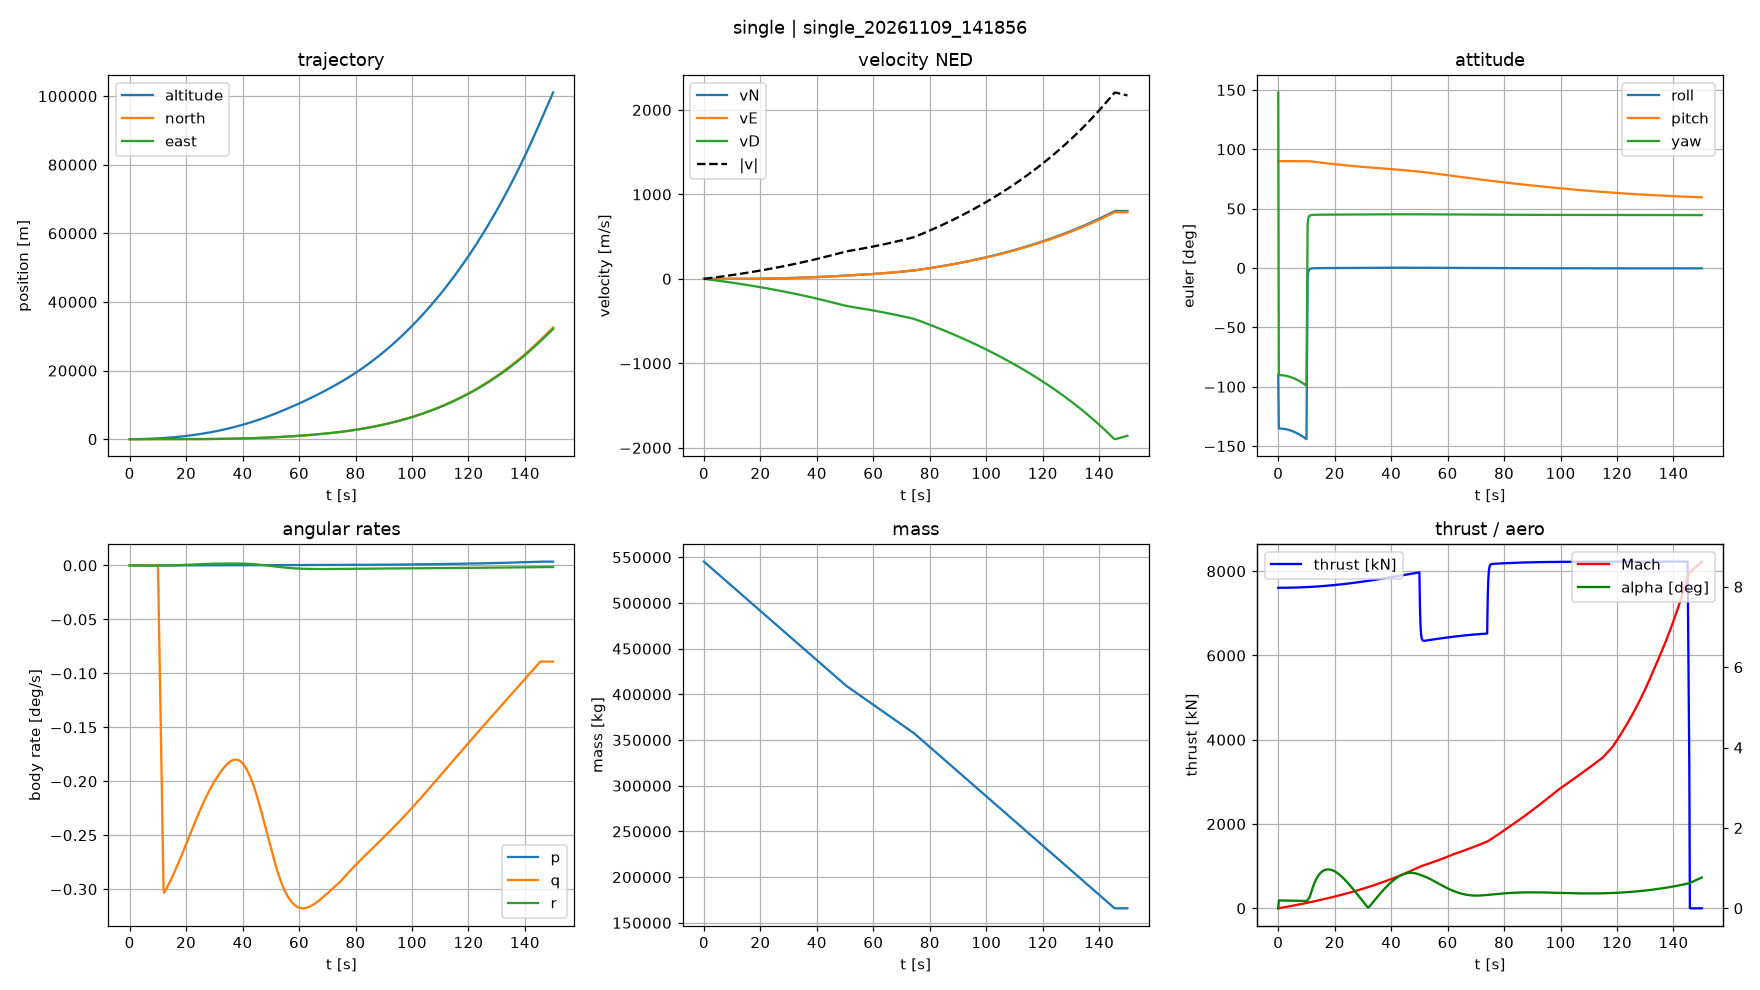
\includegraphics[width=0.97\textwidth]{images/final_runs/ascent.png}
  \caption{Executed Project~2 ascent scenario: simulator output summary.}
\end{figure}

\begin{figure}[p]
  \centering
  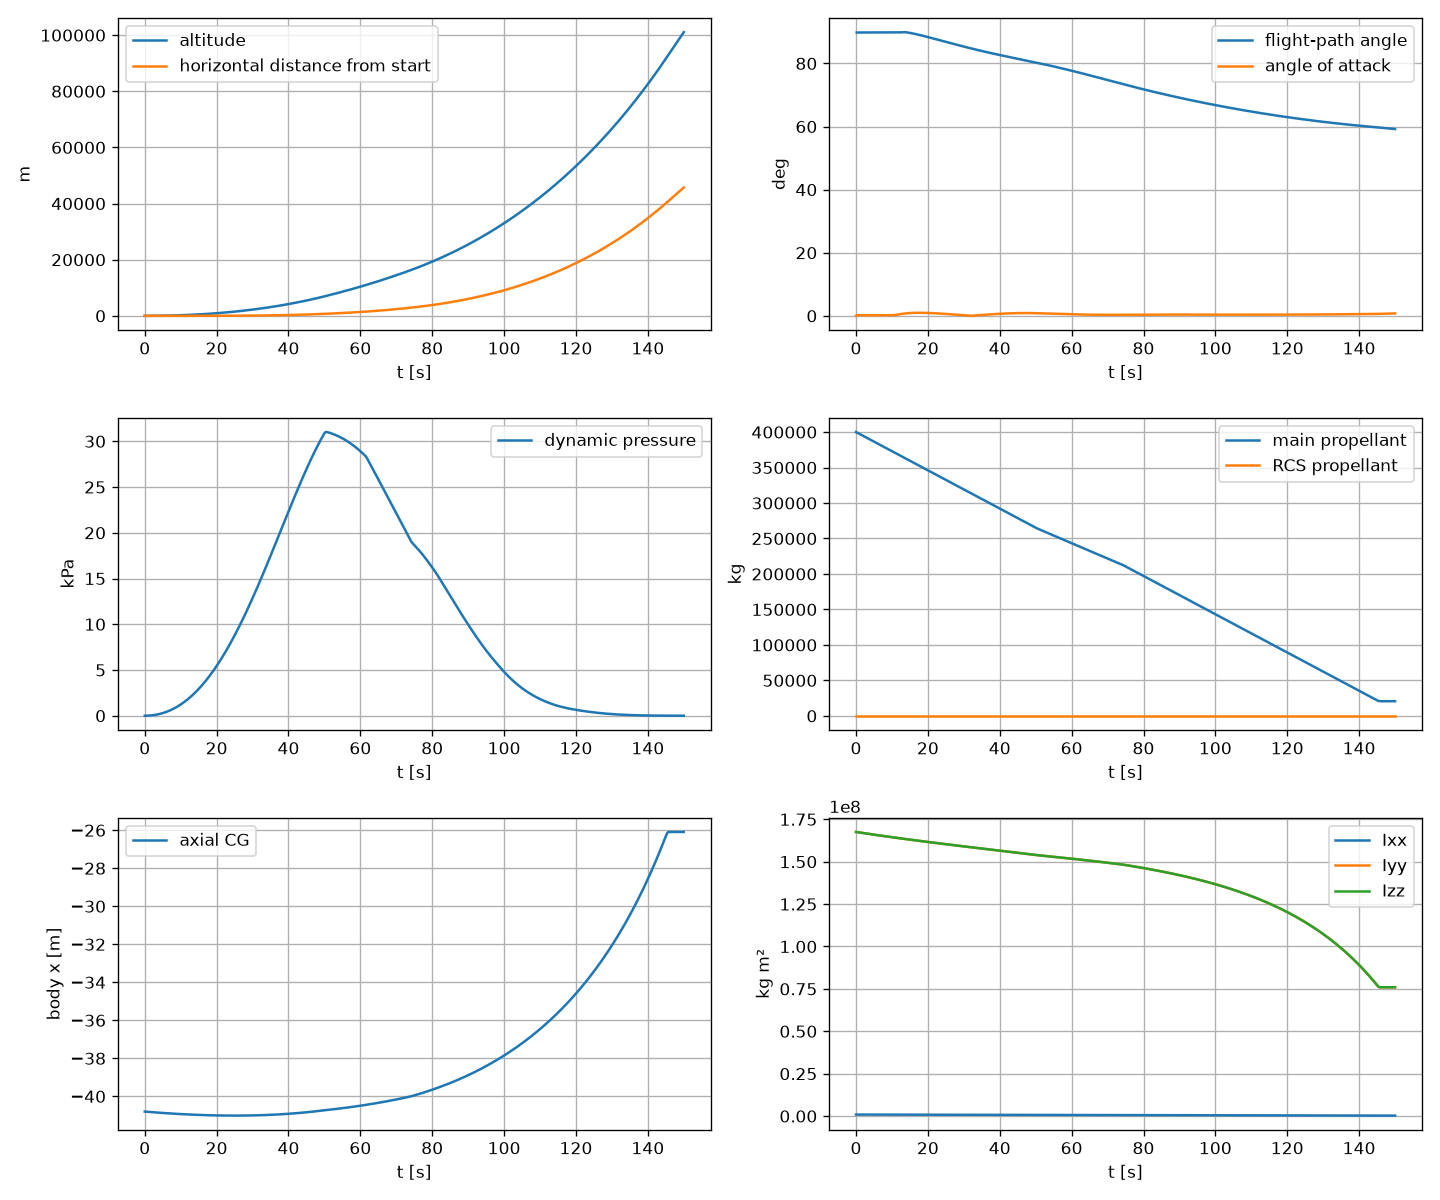
\includegraphics[width=0.97\textwidth]{images/final_runs/physics_ascent.png}
  \caption{Executed Project~2 ascent scenario: altitude/downrange, flight-path and angle-of-attack, dynamic pressure, propellant, centre of gravity, and inertia.}
\end{figure}

\begin{figure}[p]
  \centering
  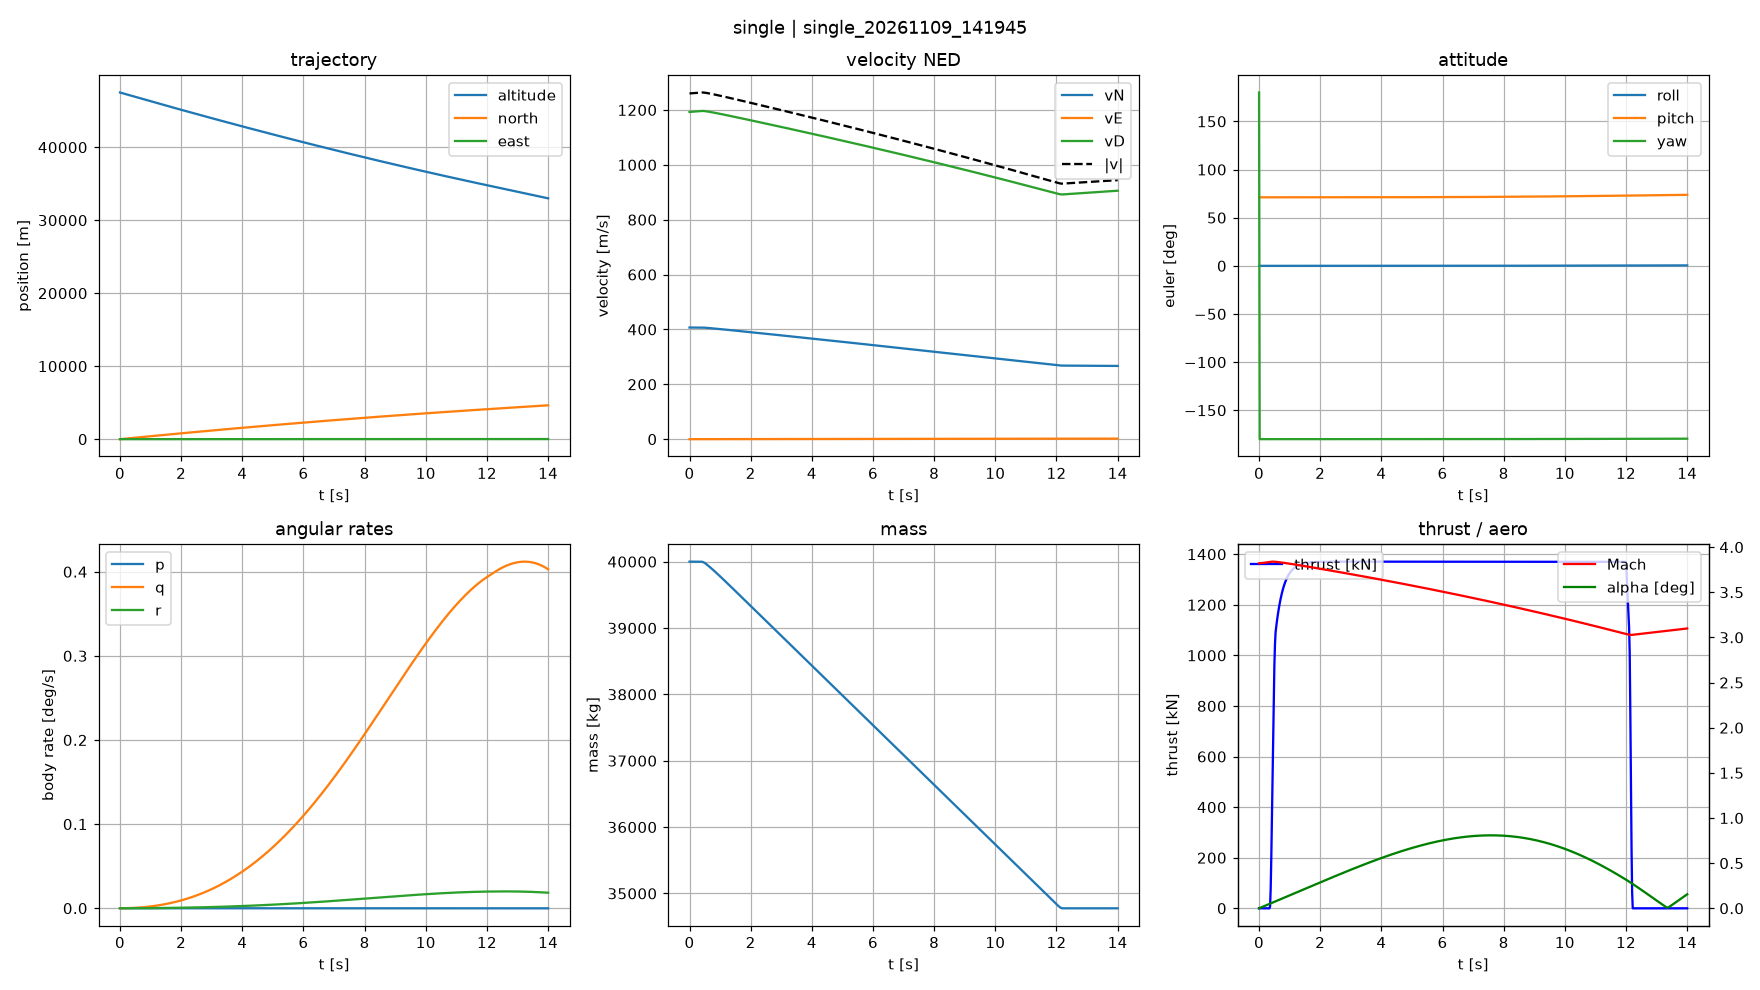
\includegraphics[width=0.97\textwidth]{images/final_runs/entry_burn.png}
  \caption{Executed Project~2 entry-burn scenario: simulator output summary.}
\end{figure}

\begin{figure}[p]
  \centering
  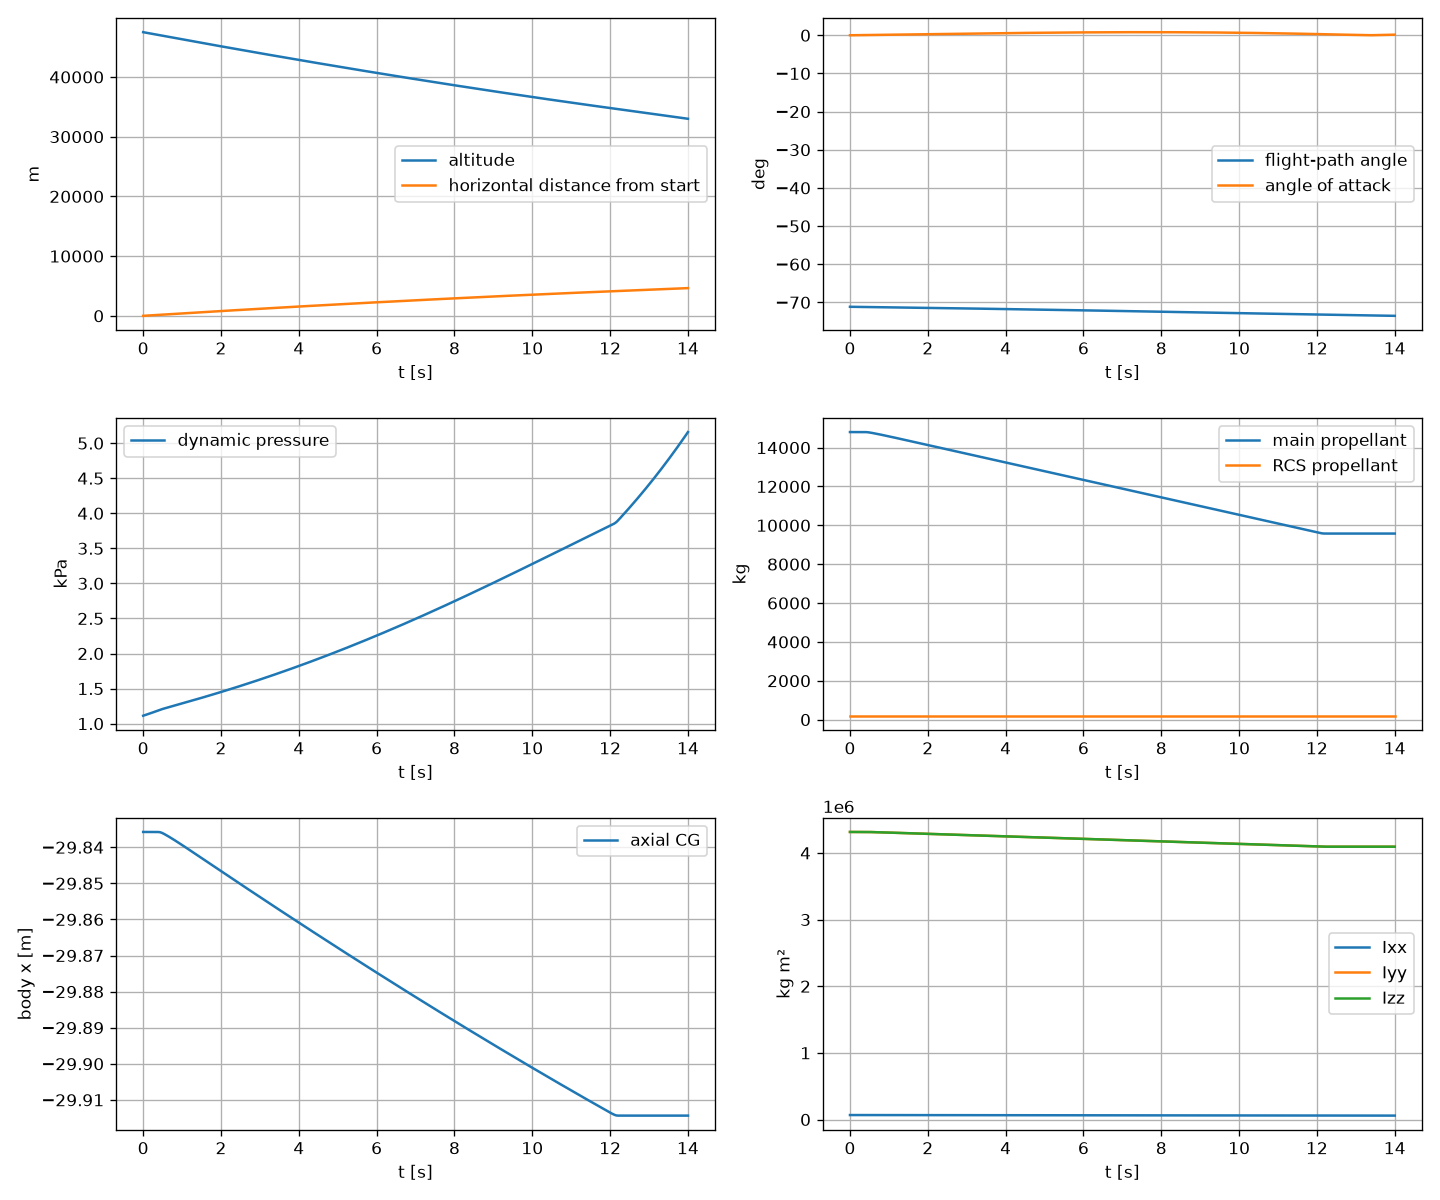
\includegraphics[width=0.97\textwidth]{images/final_runs/physics_entry_burn.png}
  \caption{Executed Project~2 entry-burn scenario: detailed physics output.}
\end{figure}

\begin{figure}[p]
  \centering
  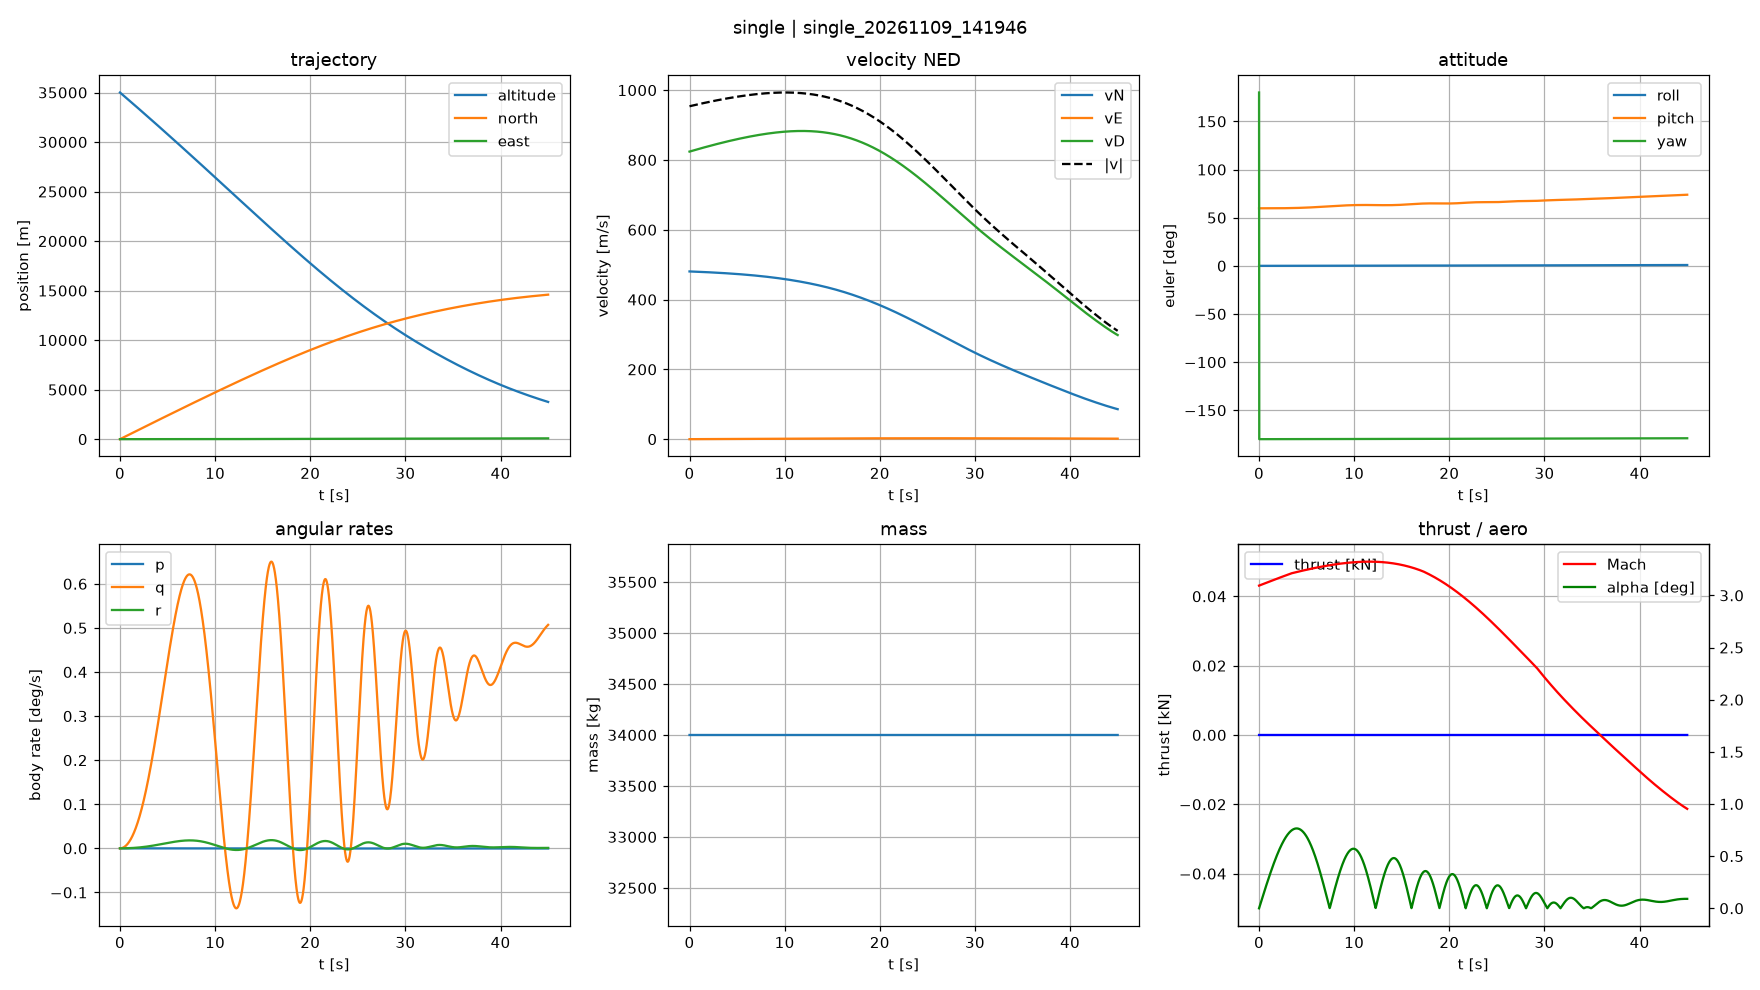
\includegraphics[width=0.97\textwidth]{images/final_runs/aero_descent.png}
  \caption{Executed Project~2 aerodynamic-descent scenario: simulator output summary.}
\end{figure}

\begin{figure}[p]
  \centering
  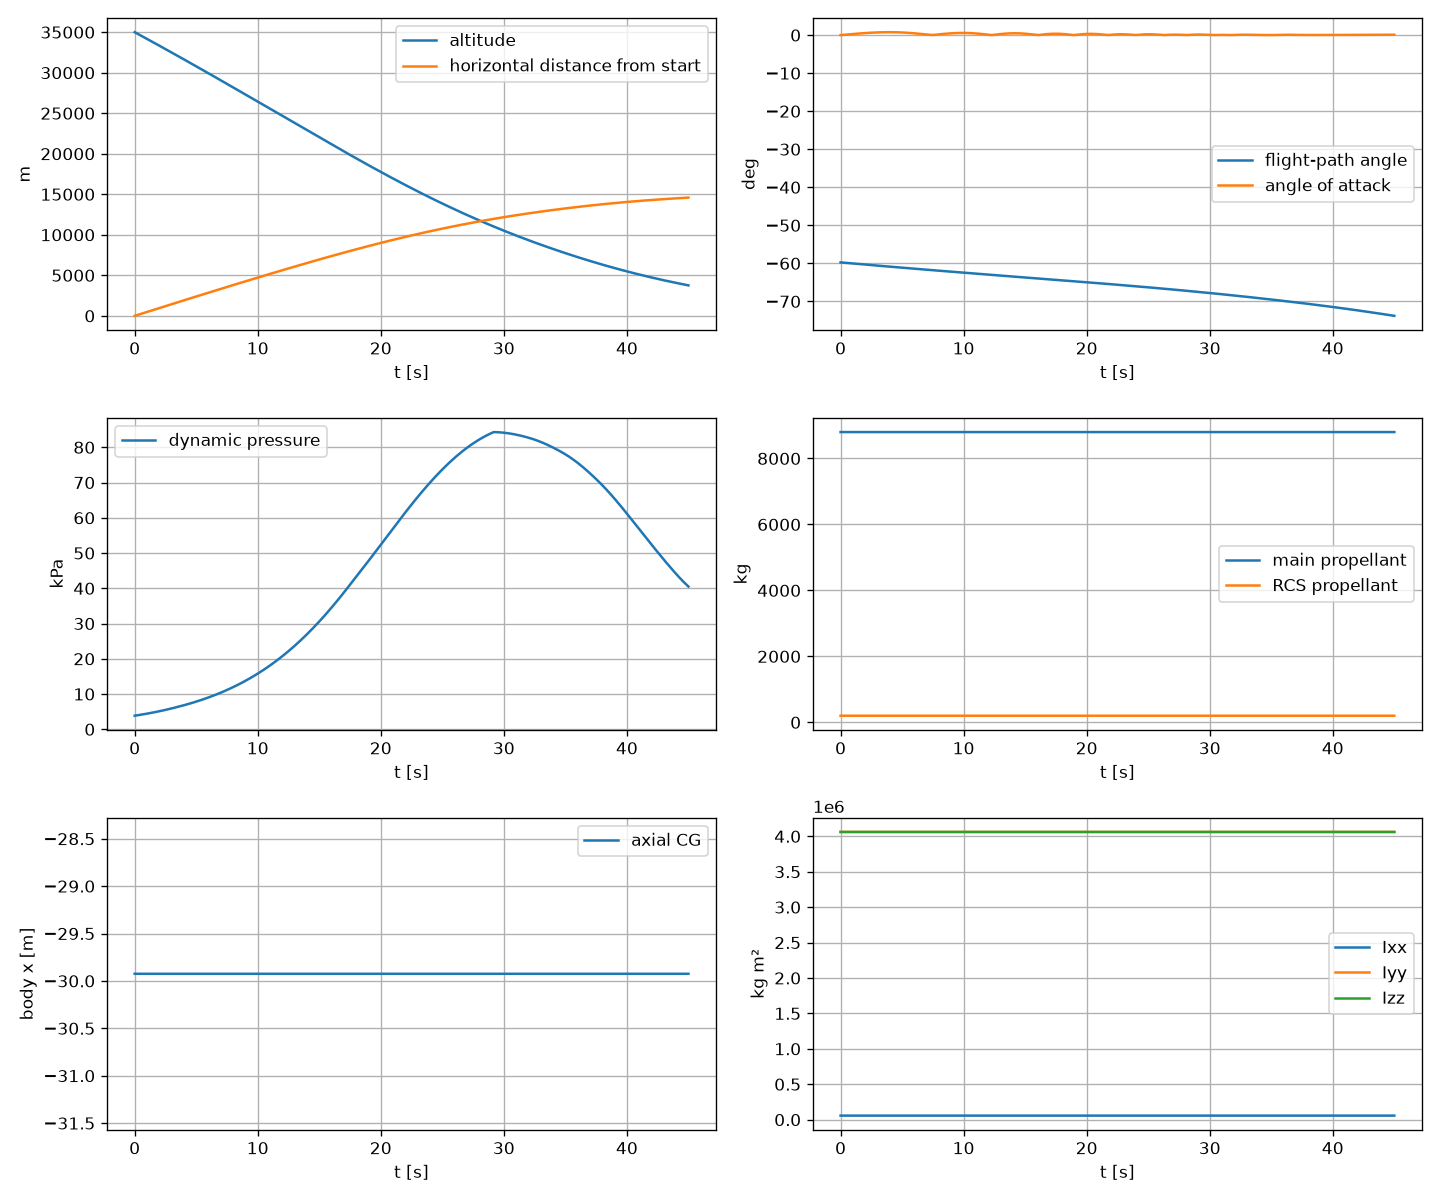
\includegraphics[width=0.97\textwidth]{images/final_runs/physics_aero_descent.png}
  \caption{Executed Project~2 aerodynamic-descent scenario: detailed physics output.}
\end{figure}

\begin{figure}[p]
  \centering
  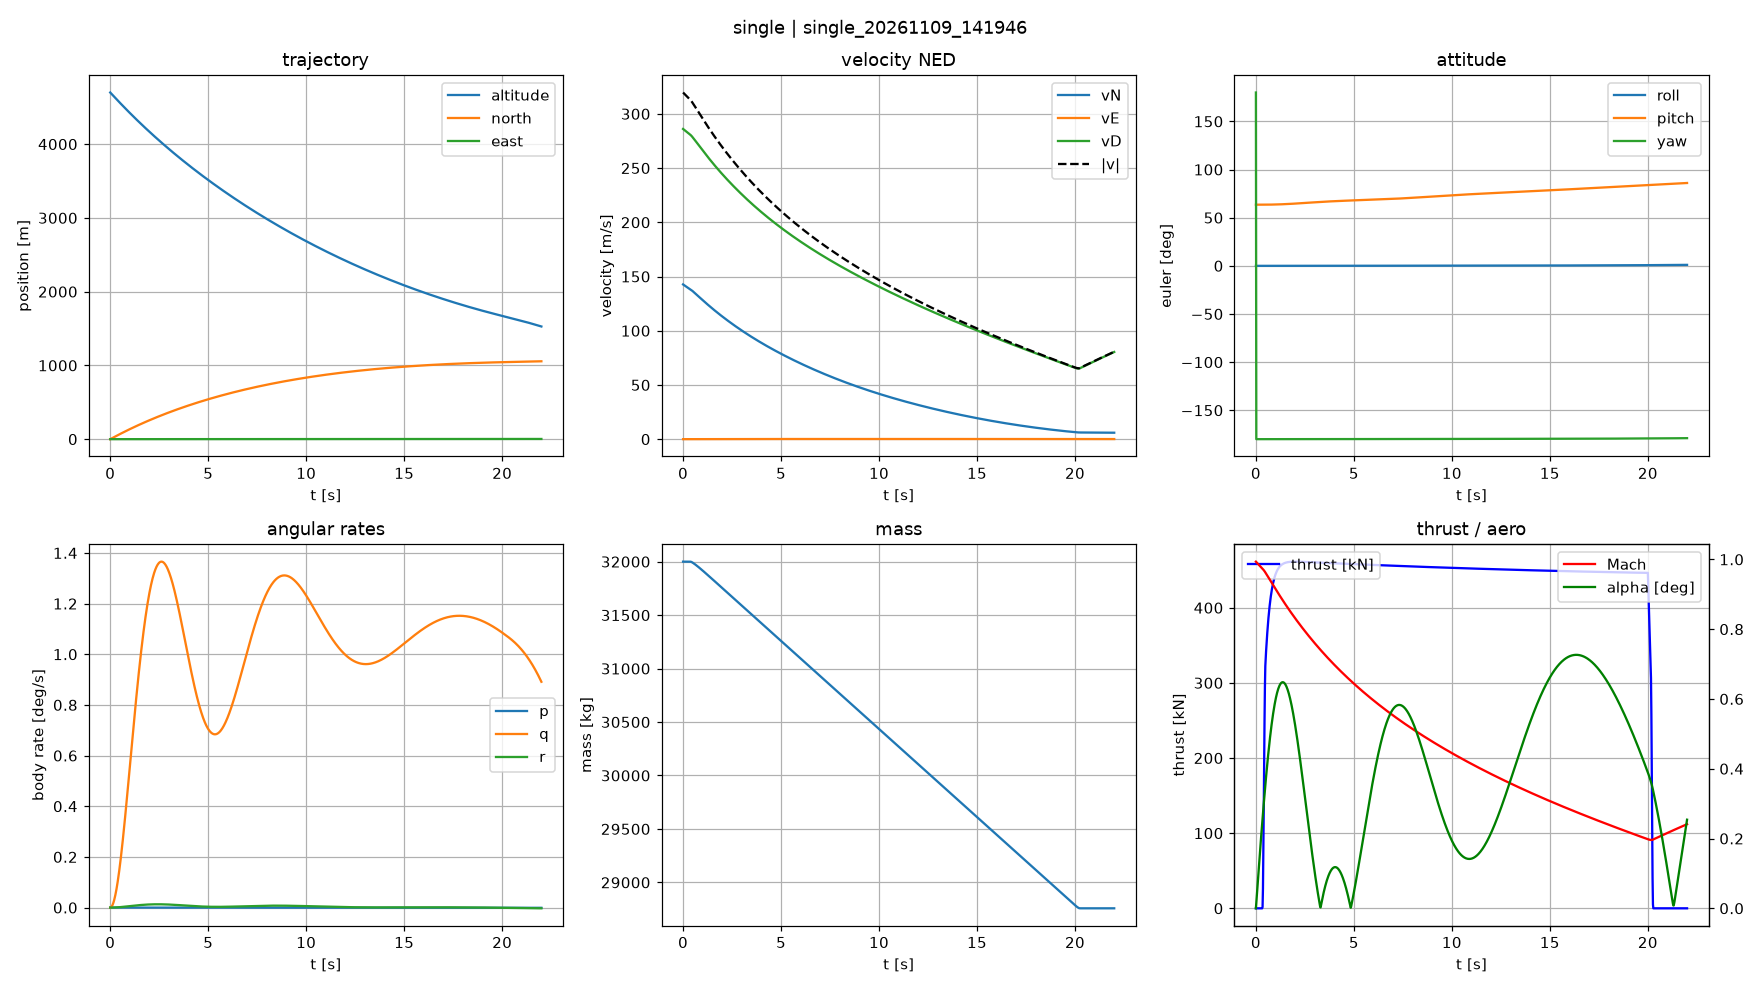
\includegraphics[width=0.97\textwidth]{images/final_runs/powered_descent.png}
  \caption{Executed Project~2 powered-descent scenario: simulator output summary.}
\end{figure}

\begin{figure}[p]
  \centering
  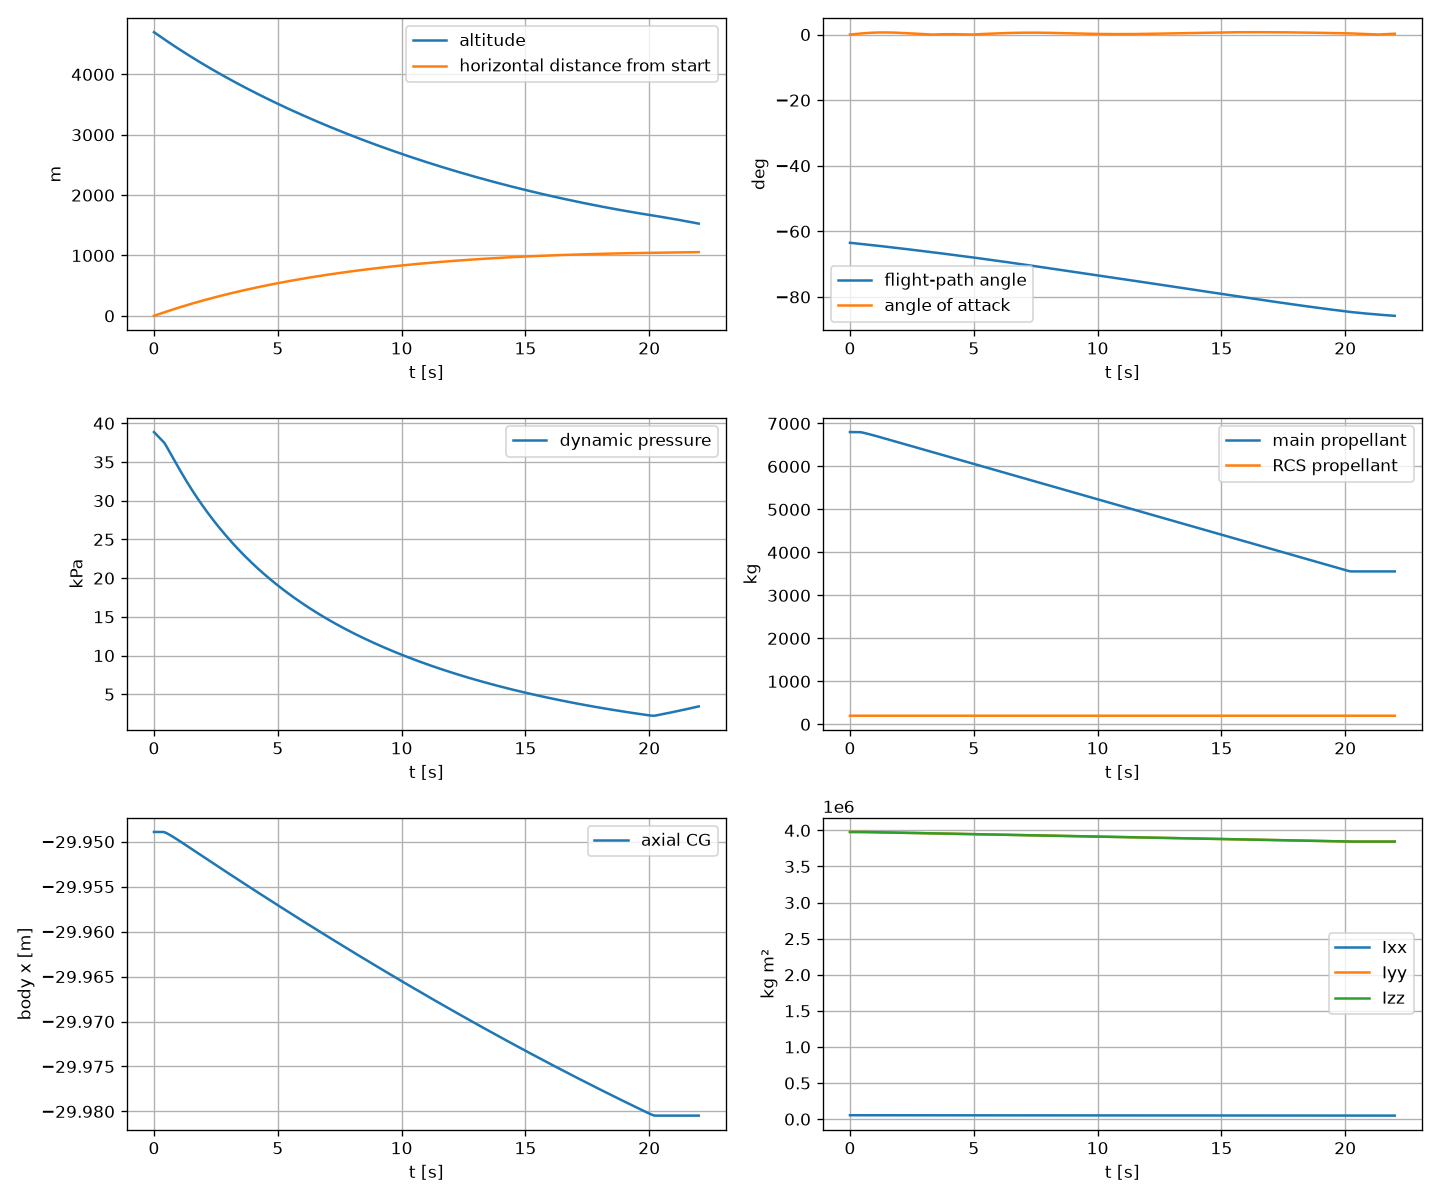
\includegraphics[width=0.97\textwidth]{images/final_runs/physics_powered_descent.png}
  \caption{Executed Project~2 powered-descent scenario: detailed physics output.}
\end{figure}

\begin{figure}[p]
  \centering
  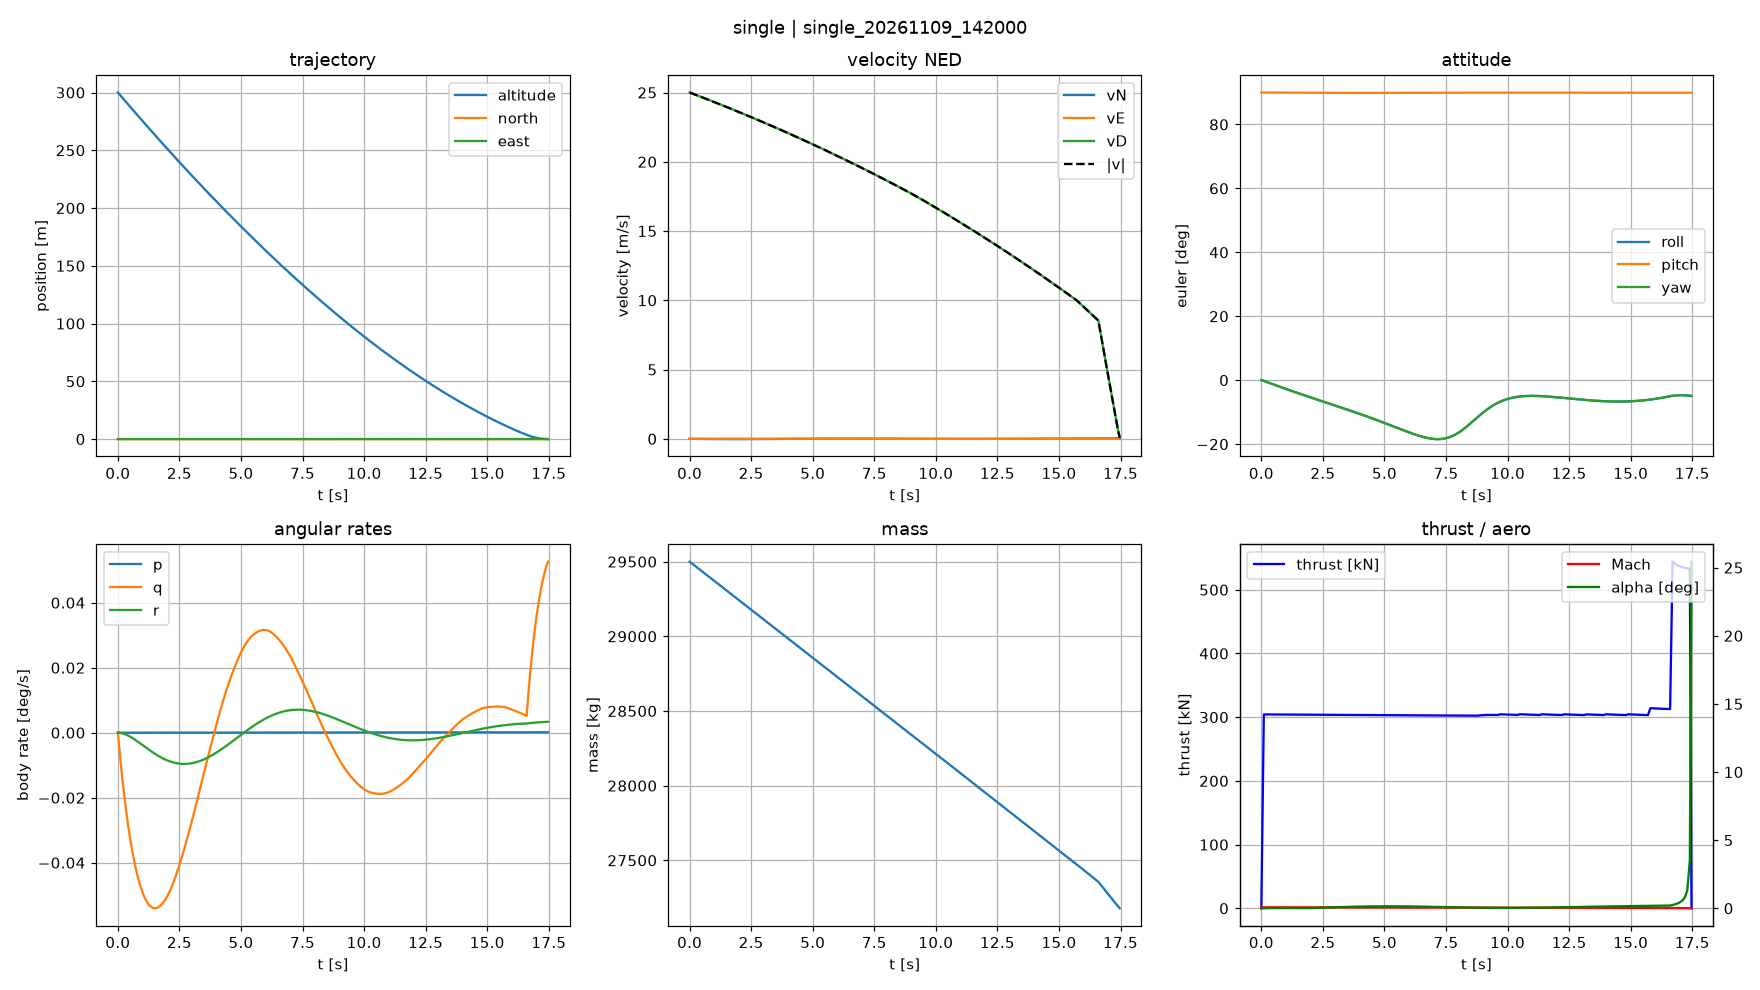
\includegraphics[width=0.97\textwidth]{images/final_runs/landing.png}
  \caption{Executed Project~2 closed-loop landing scenario: simulator output summary.}
\end{figure}

\begin{figure}[p]
  \centering
  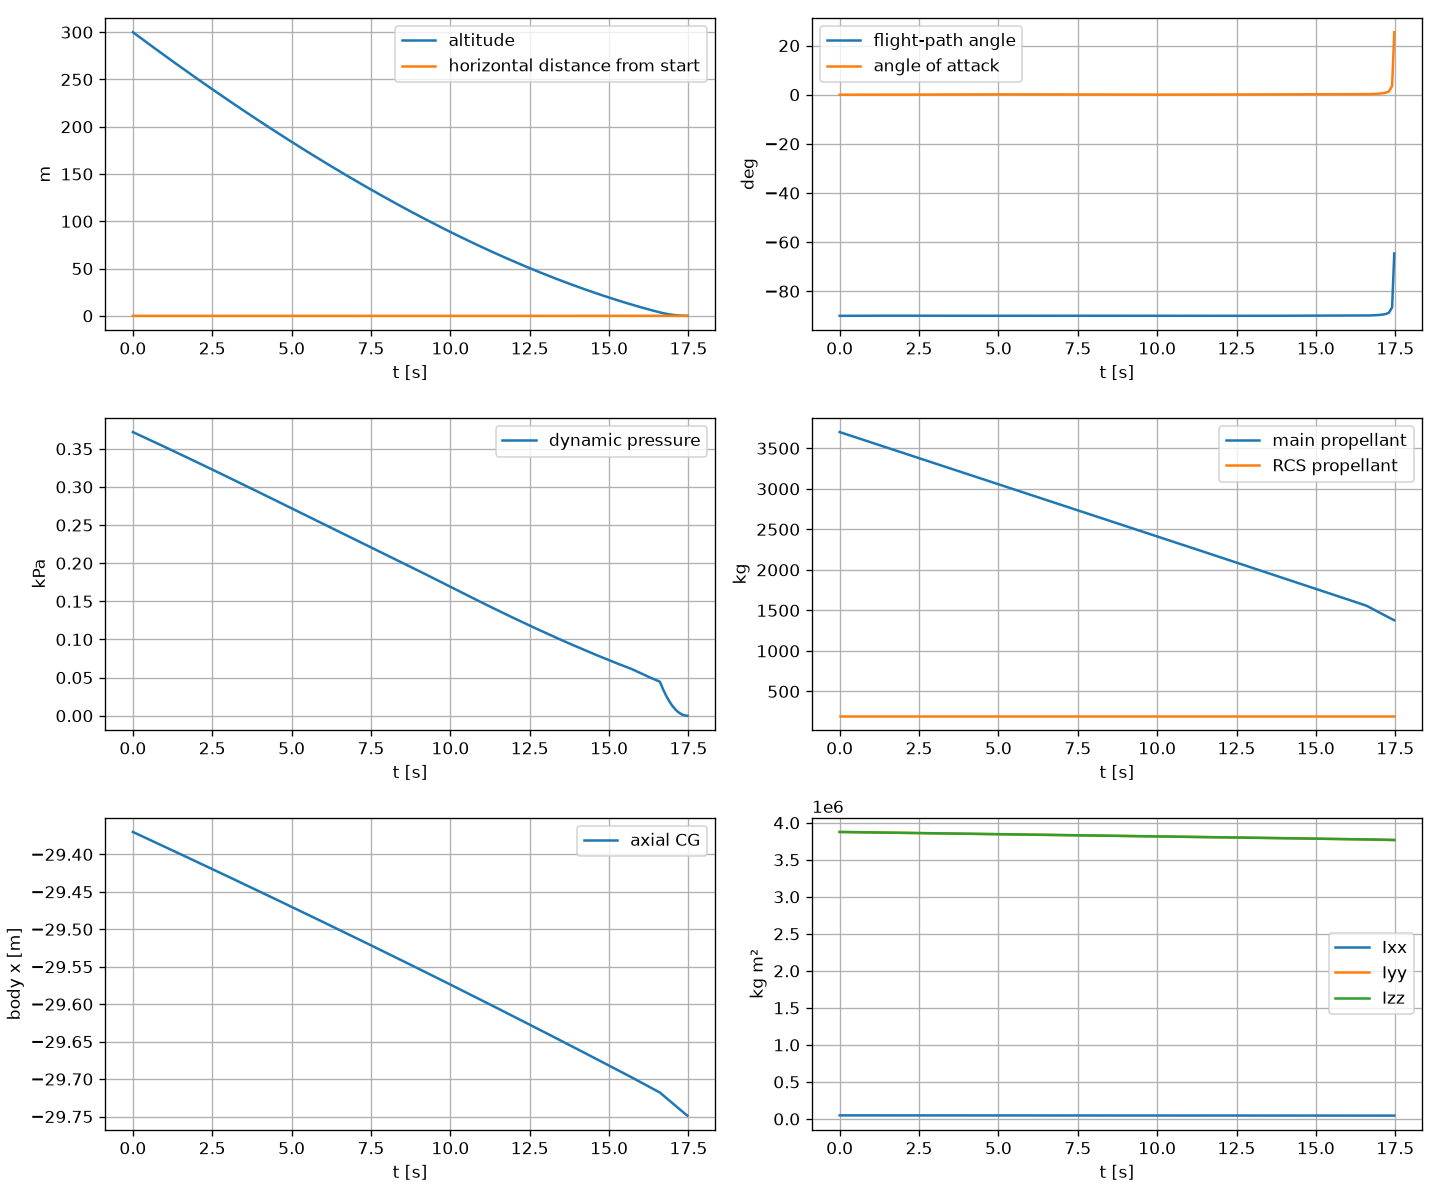
\includegraphics[width=0.97\textwidth]{images/final_runs/physics_landing.png}
  \caption{Executed Project~2 closed-loop landing scenario: detailed physics output.}
\end{figure}

\clearpage
\section{Executed CRS-11 Observable-Comparison Plots}\label{app:comparisonplots}

These figures show the archive's optional, source-defined comparison between each executed scenario and the supplied CRS-11 reconstruction. They are included to make the RMSE values in Table~\ref{tab:flight-rmse} inspectable. They do not represent navigation-filter errors.

\begin{figure}[p]
  \centering
  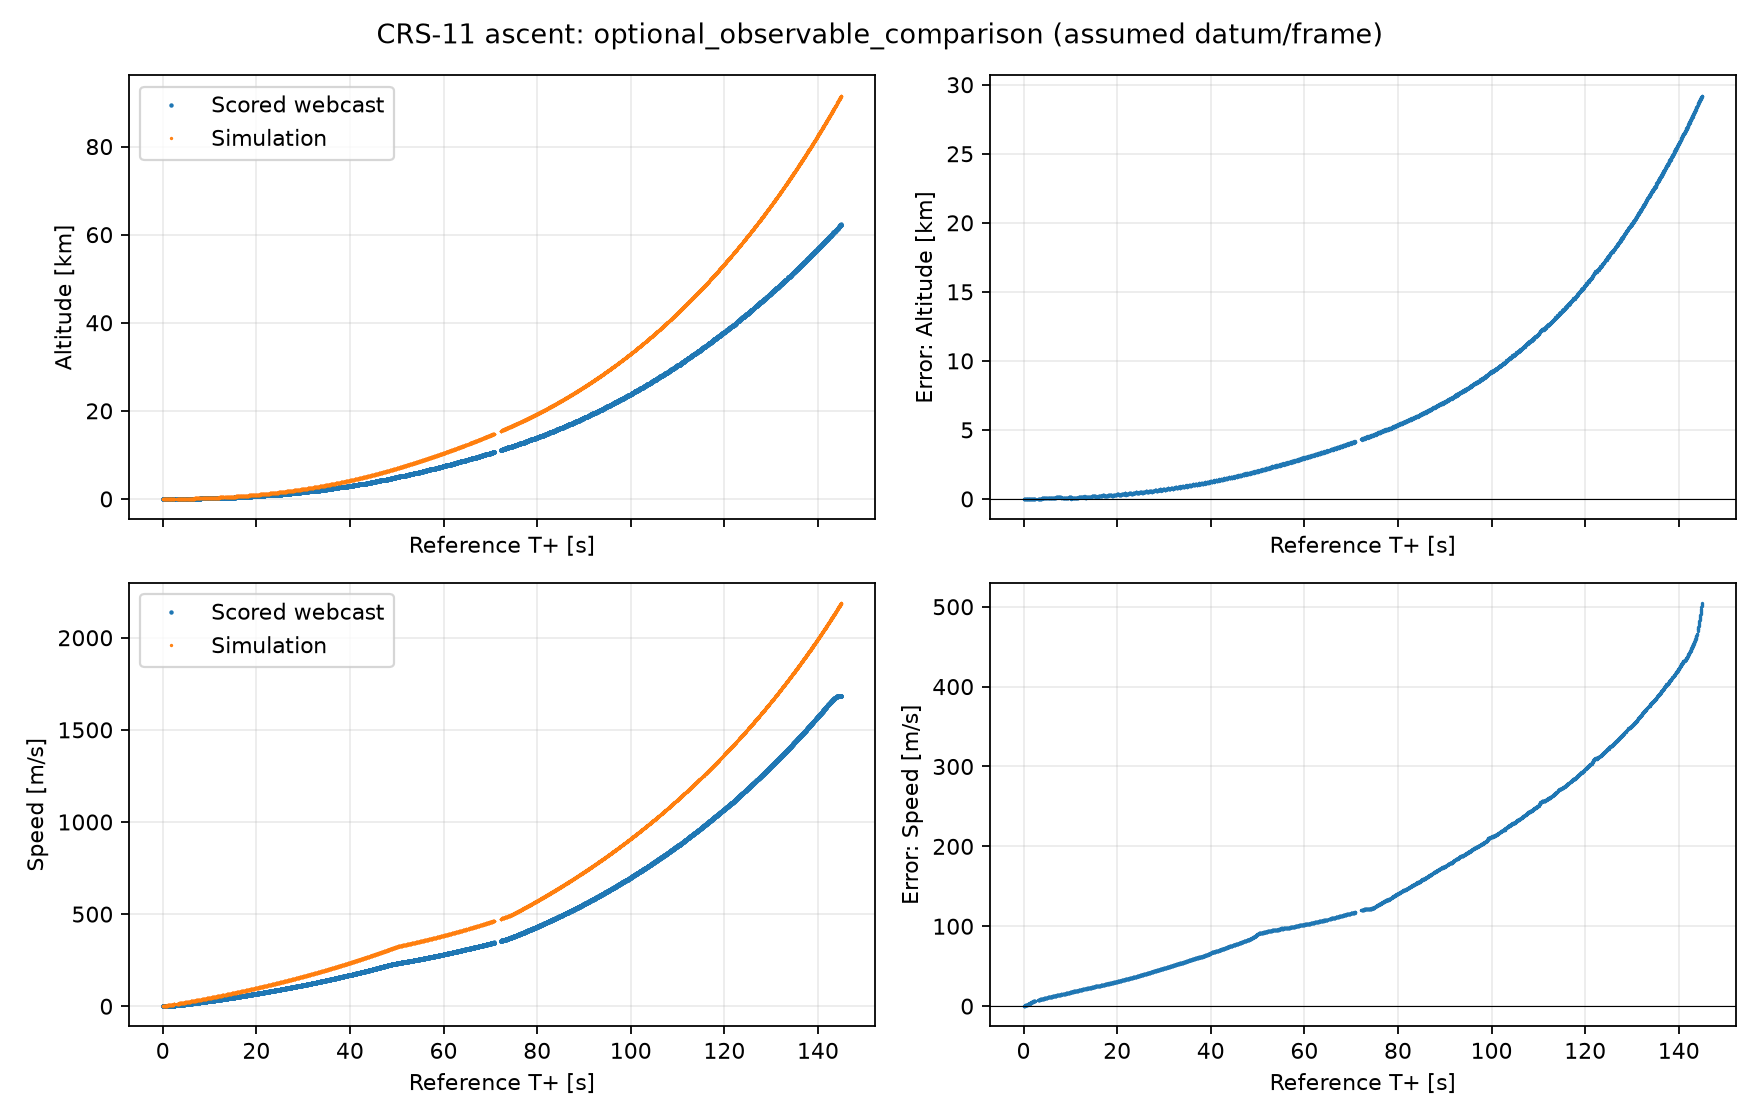
\includegraphics[width=0.97\textwidth]{images/final_runs/comparison_ascent.png}
  \caption{Executed observable comparison: Project~2 ascent and CRS-11 reconstruction.}
\end{figure}

\begin{figure}[p]
  \centering
  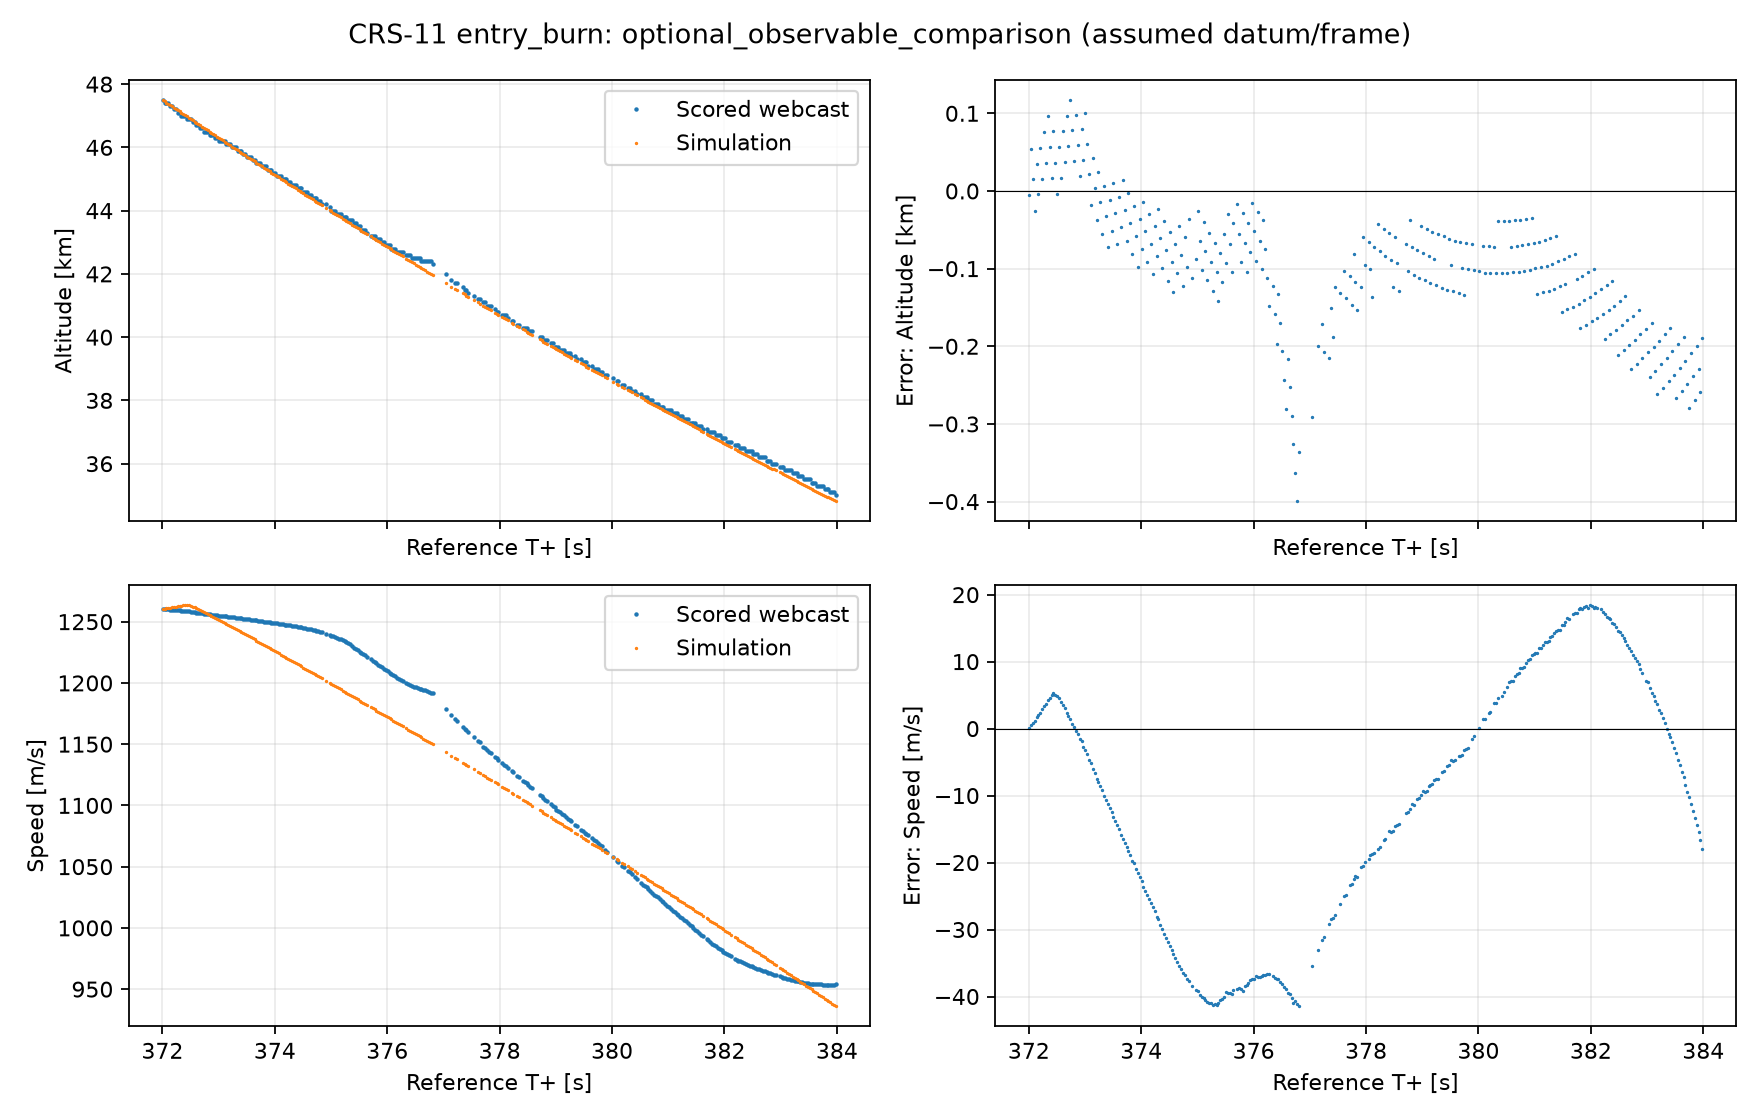
\includegraphics[width=0.97\textwidth]{images/final_runs/comparison_entry_burn.png}
  \caption{Executed observable comparison: Project~2 entry burn and CRS-11 reconstruction.}
\end{figure}

\begin{figure}[p]
  \centering
  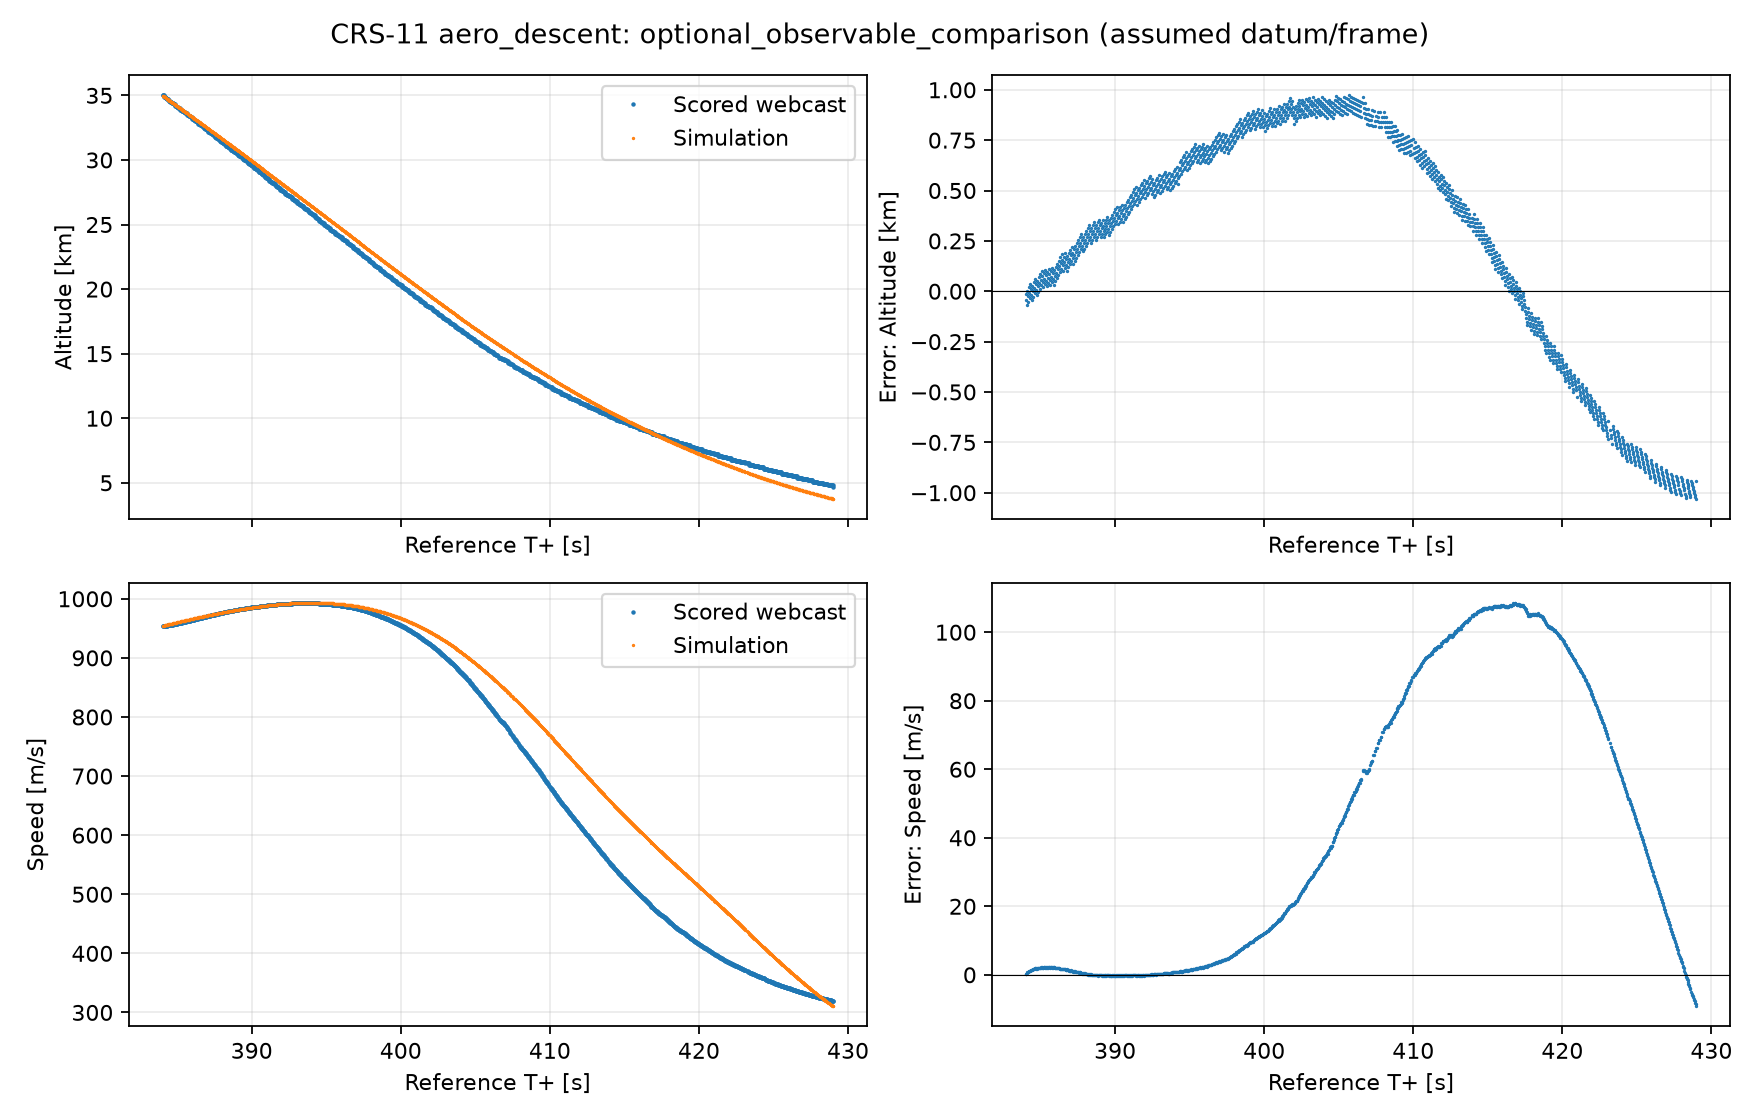
\includegraphics[width=0.97\textwidth]{images/final_runs/comparison_aero_descent.png}
  \caption{Executed observable comparison: Project~2 aerodynamic descent and CRS-11 reconstruction.}
\end{figure}

\begin{figure}[p]
  \centering
  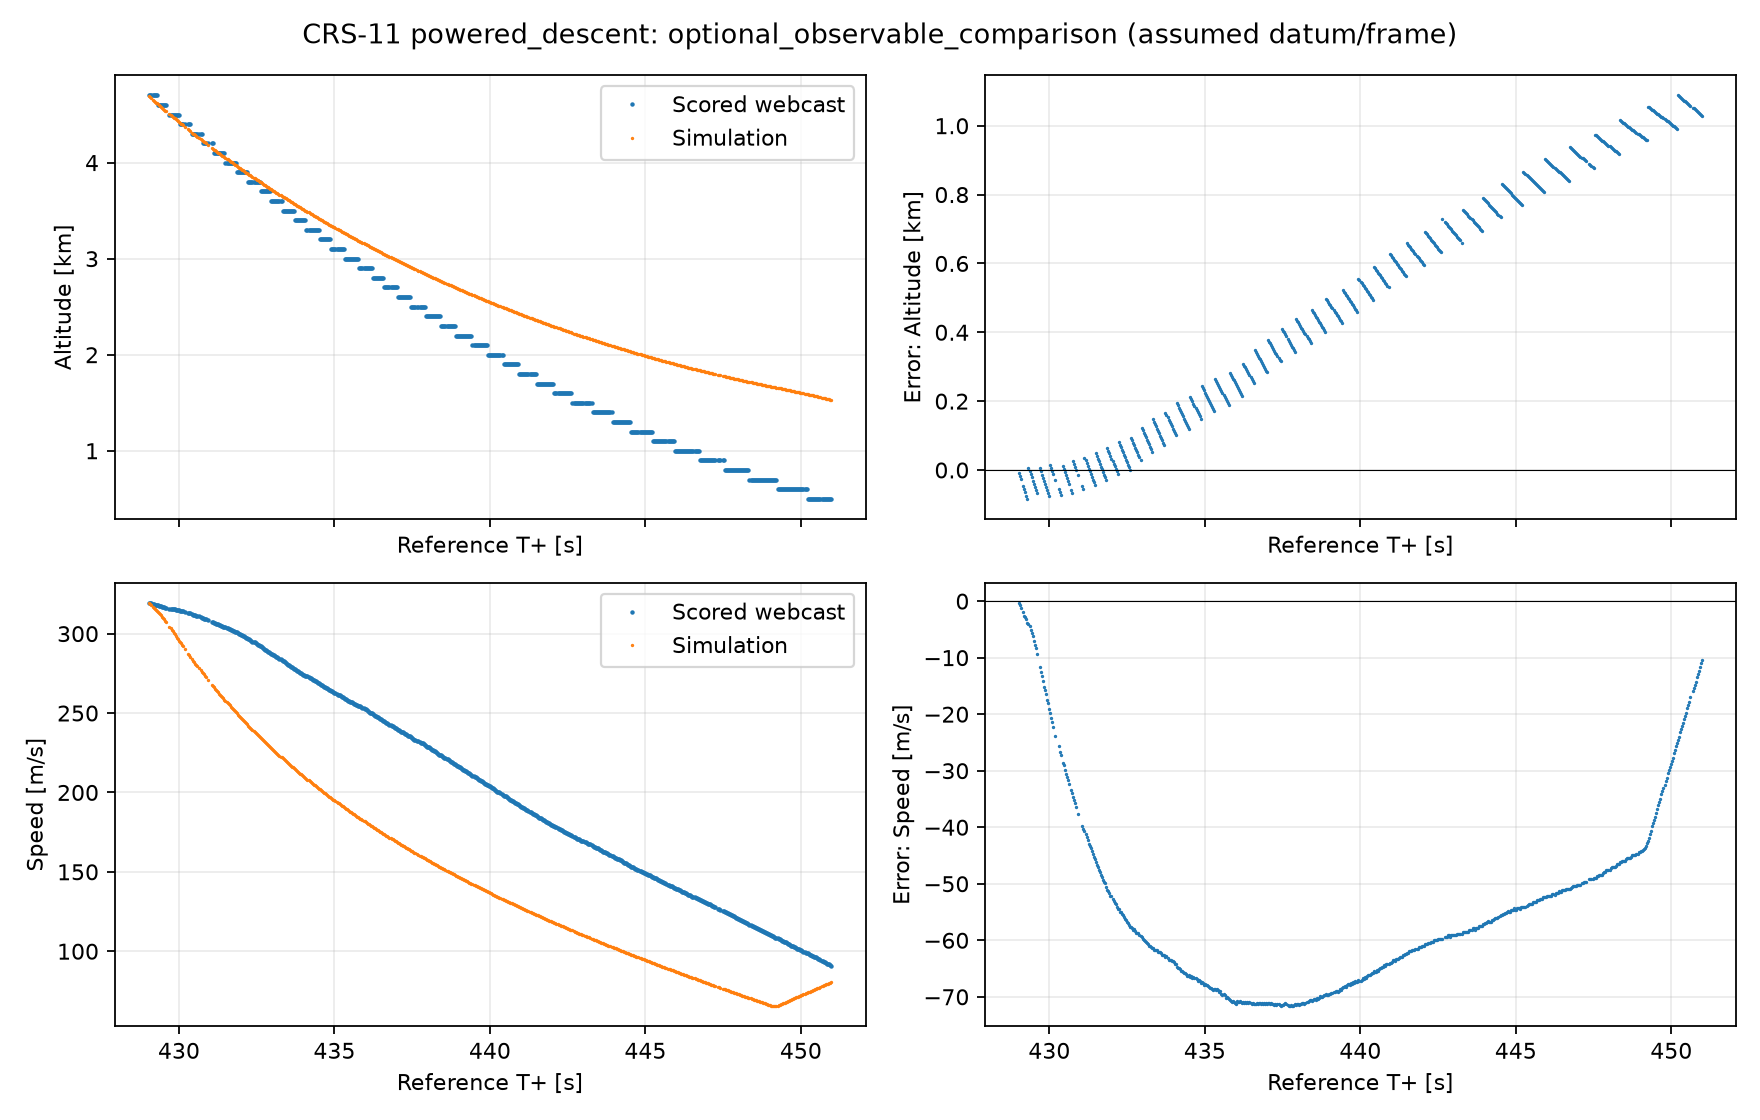
\includegraphics[width=0.97\textwidth]{images/final_runs/comparison_powered_descent.png}
  \caption{Executed observable comparison: Project~2 powered descent and CRS-11 reconstruction.}
\end{figure}

\clearpage
\section{CRS-11 Reference Plots}

The following plots are the team-supplied webcast reconstruction. They are included as reference context only. They should be captioned as reconstructed observables, not as simulator output.

\begin{figure}[p]
  \centering
  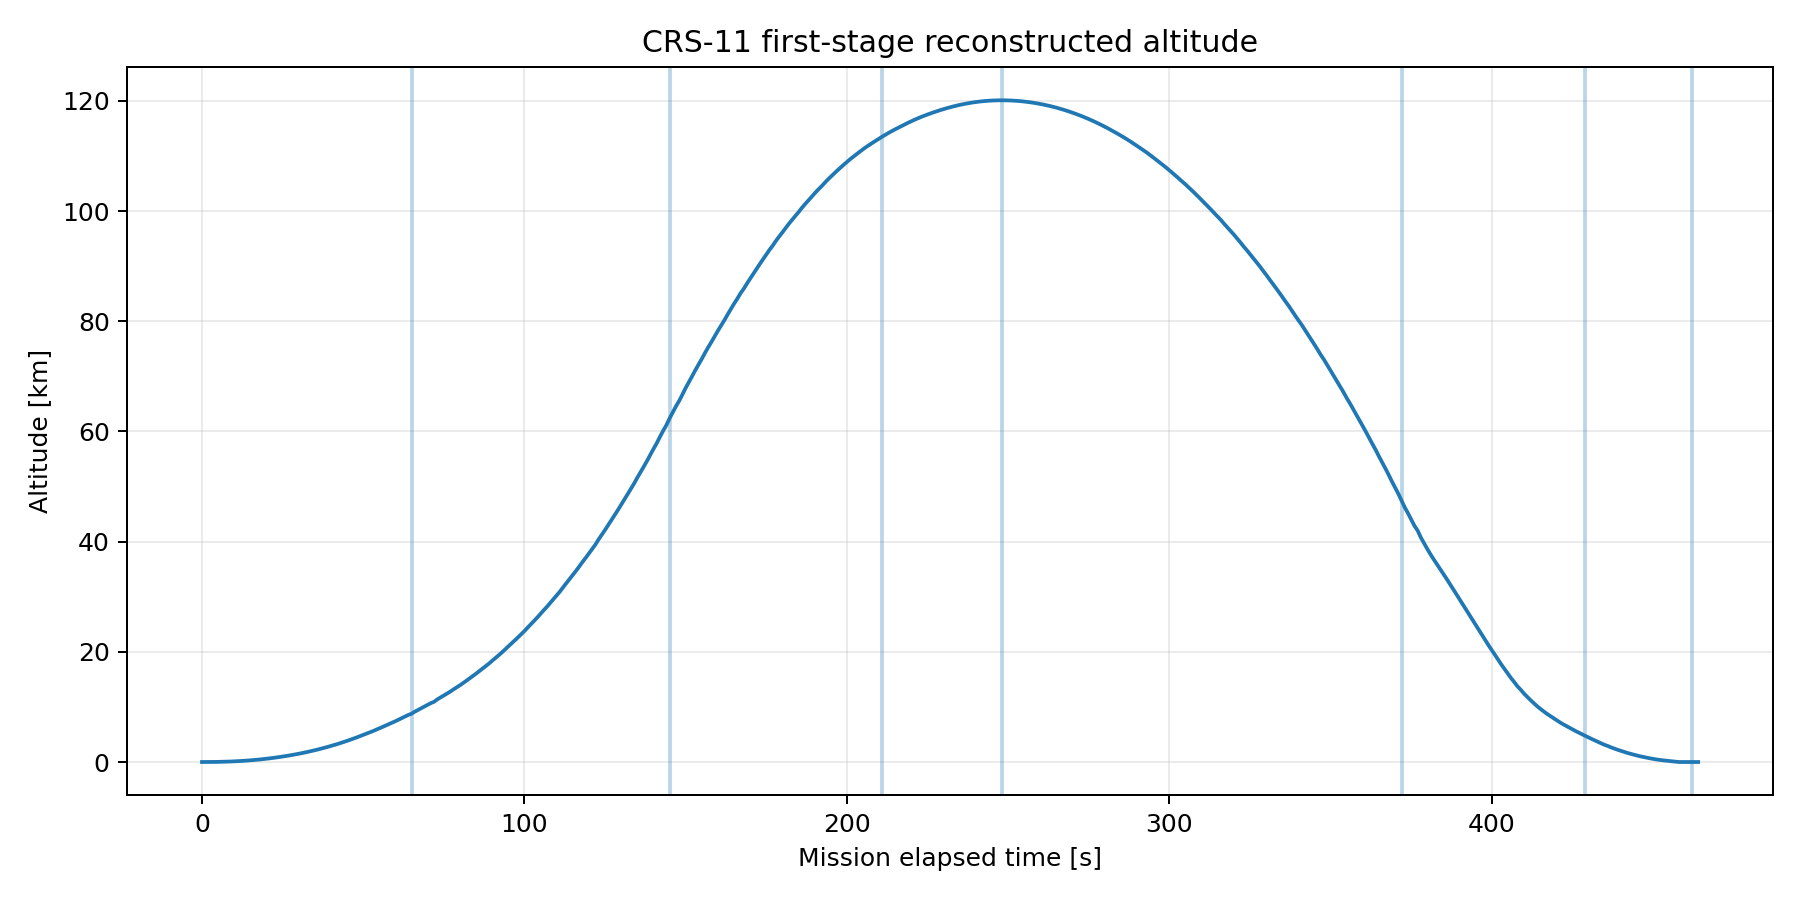
\includegraphics[width=0.97\textwidth]{images/crs11_altitude_time.png}
  \caption{CRS-11 reconstructed altitude versus mission elapsed time. Source: team-supplied webcast reconstruction~\cite{crs11}.}
\end{figure}

\begin{figure}[p]
  \centering
  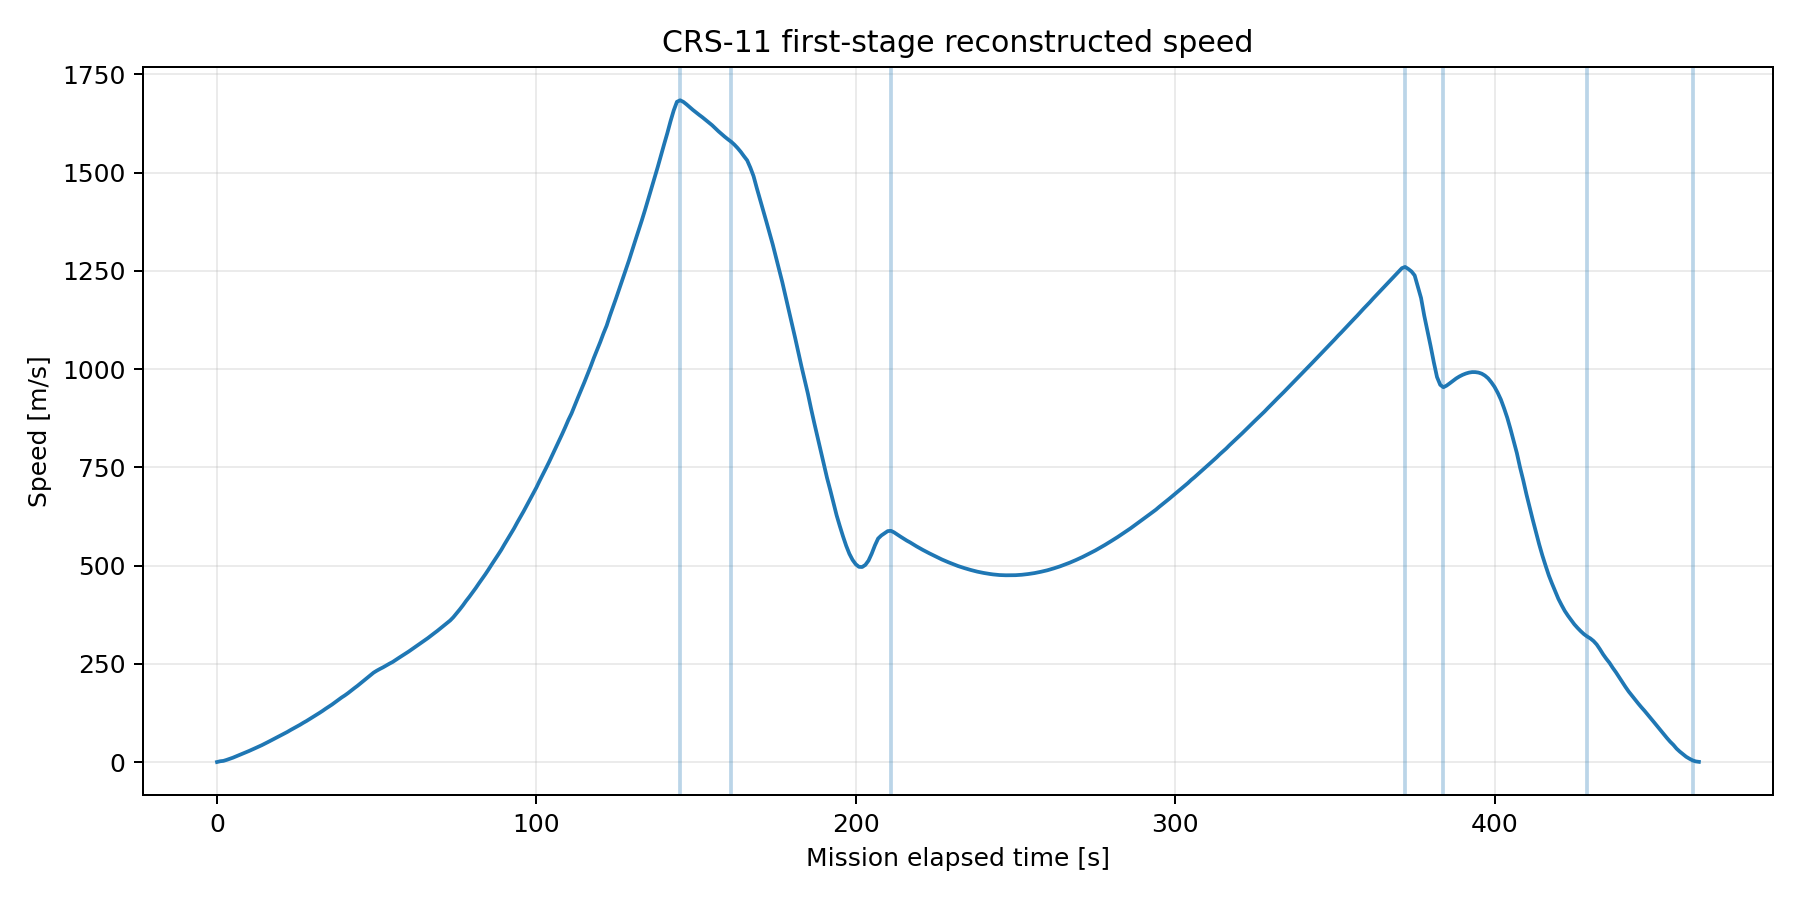
\includegraphics[width=0.97\textwidth]{images/crs11_velocity_time.png}
  \caption{CRS-11 reconstructed speed versus mission elapsed time. Source: team-supplied webcast reconstruction~\cite{crs11}.}
\end{figure}

\begin{figure}[p]
  \centering
  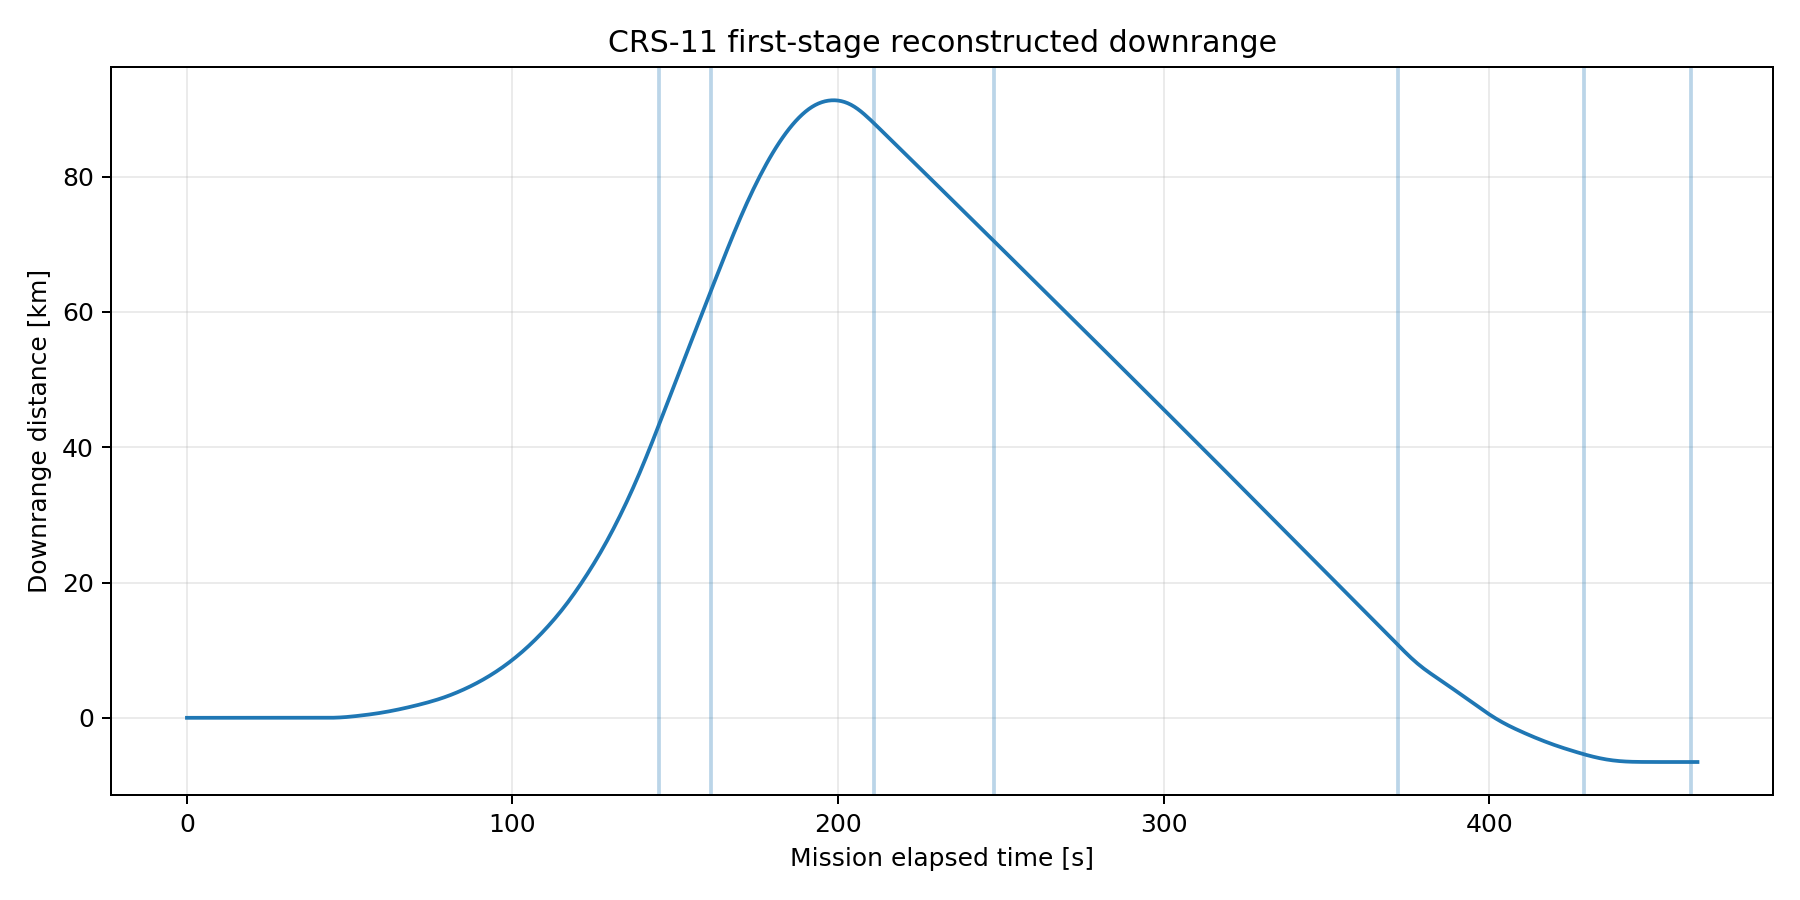
\includegraphics[width=0.97\textwidth]{images/crs11_downrange_time.png}
  \caption{CRS-11 reconstructed downrange distance versus mission elapsed time. Source: team-supplied webcast reconstruction~\cite{crs11}.}
\end{figure}

\begin{figure}[p]
  \centering
  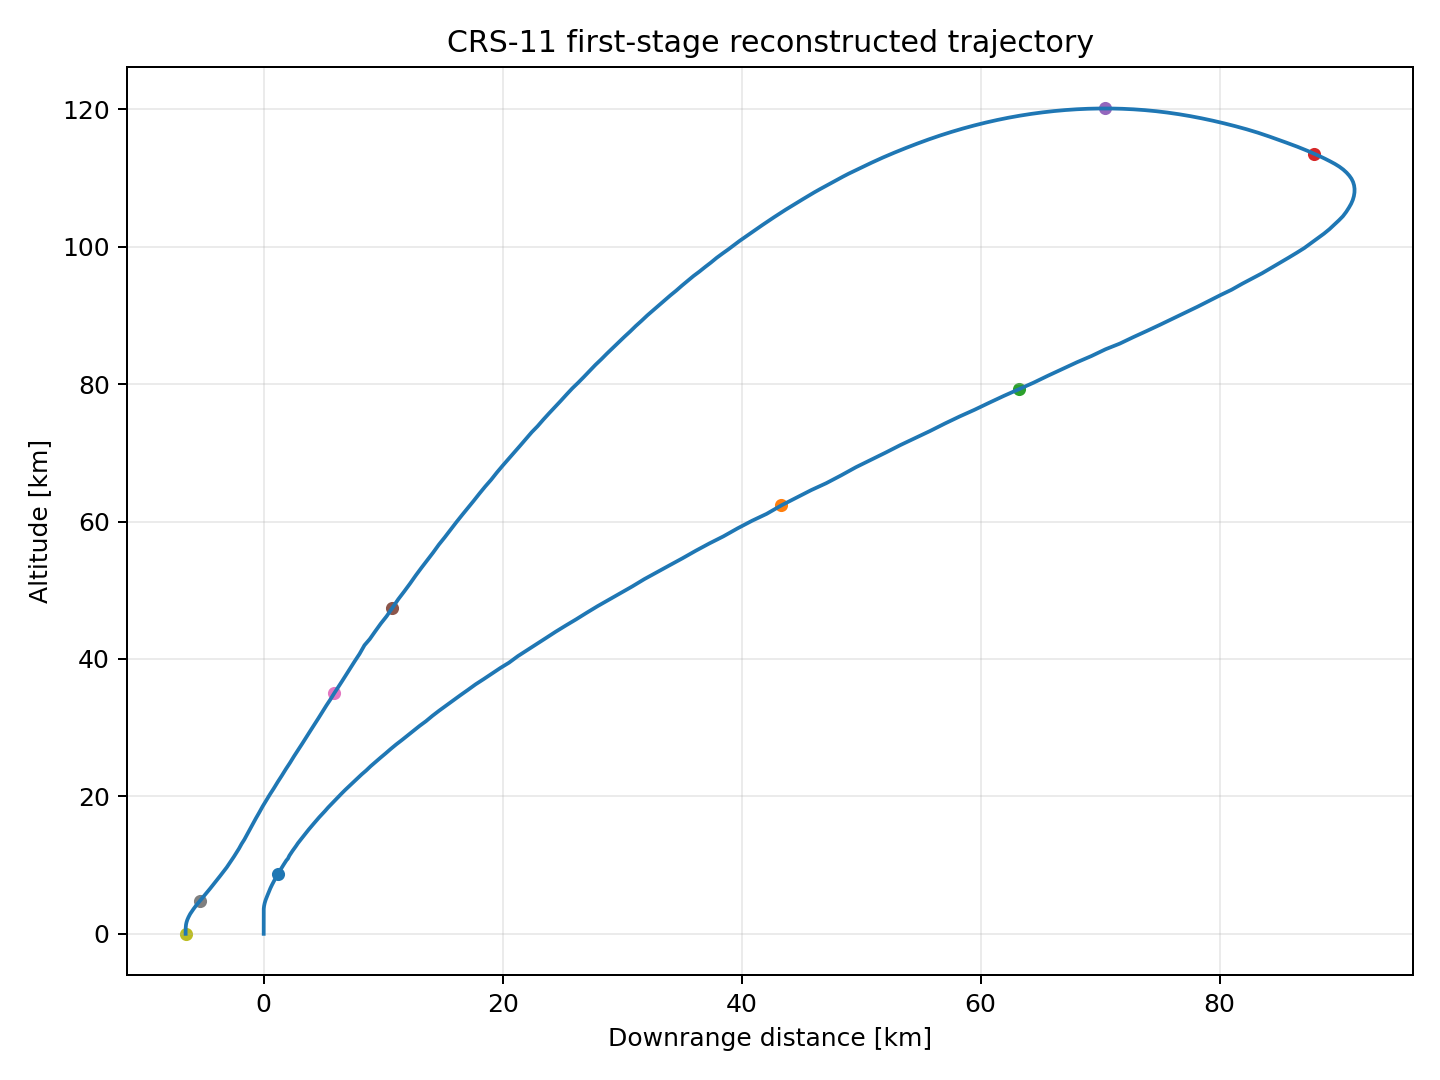
\includegraphics[width=0.97\textwidth]{images/crs11_trajectory_2D.png}
  \caption{CRS-11 reconstructed altitude-downrange trajectory. Source: team-supplied webcast reconstruction~\cite{crs11}.}
\end{figure}

\clearpage
\section{Synthetic Navigation Comparison Plots}\label{app:navplots}

These plots are from the fixed-truth seeded analysis described in Section~\ref{sec:verification}.
The black trajectory is the simulated 6-DOF truth reference; the INS-only and aided ESKF estimates
use the same truth initial state and synthetic measurement sequence. They are not CRS-11 flight
data. The analysis used 200~Hz IMU, 10~Hz GNSS, and 20~Hz radar updates, including a scheduled
8--12~s GNSS outage and a GNSS outlier at 4~s.

\begin{figure}[p]
  \centering
  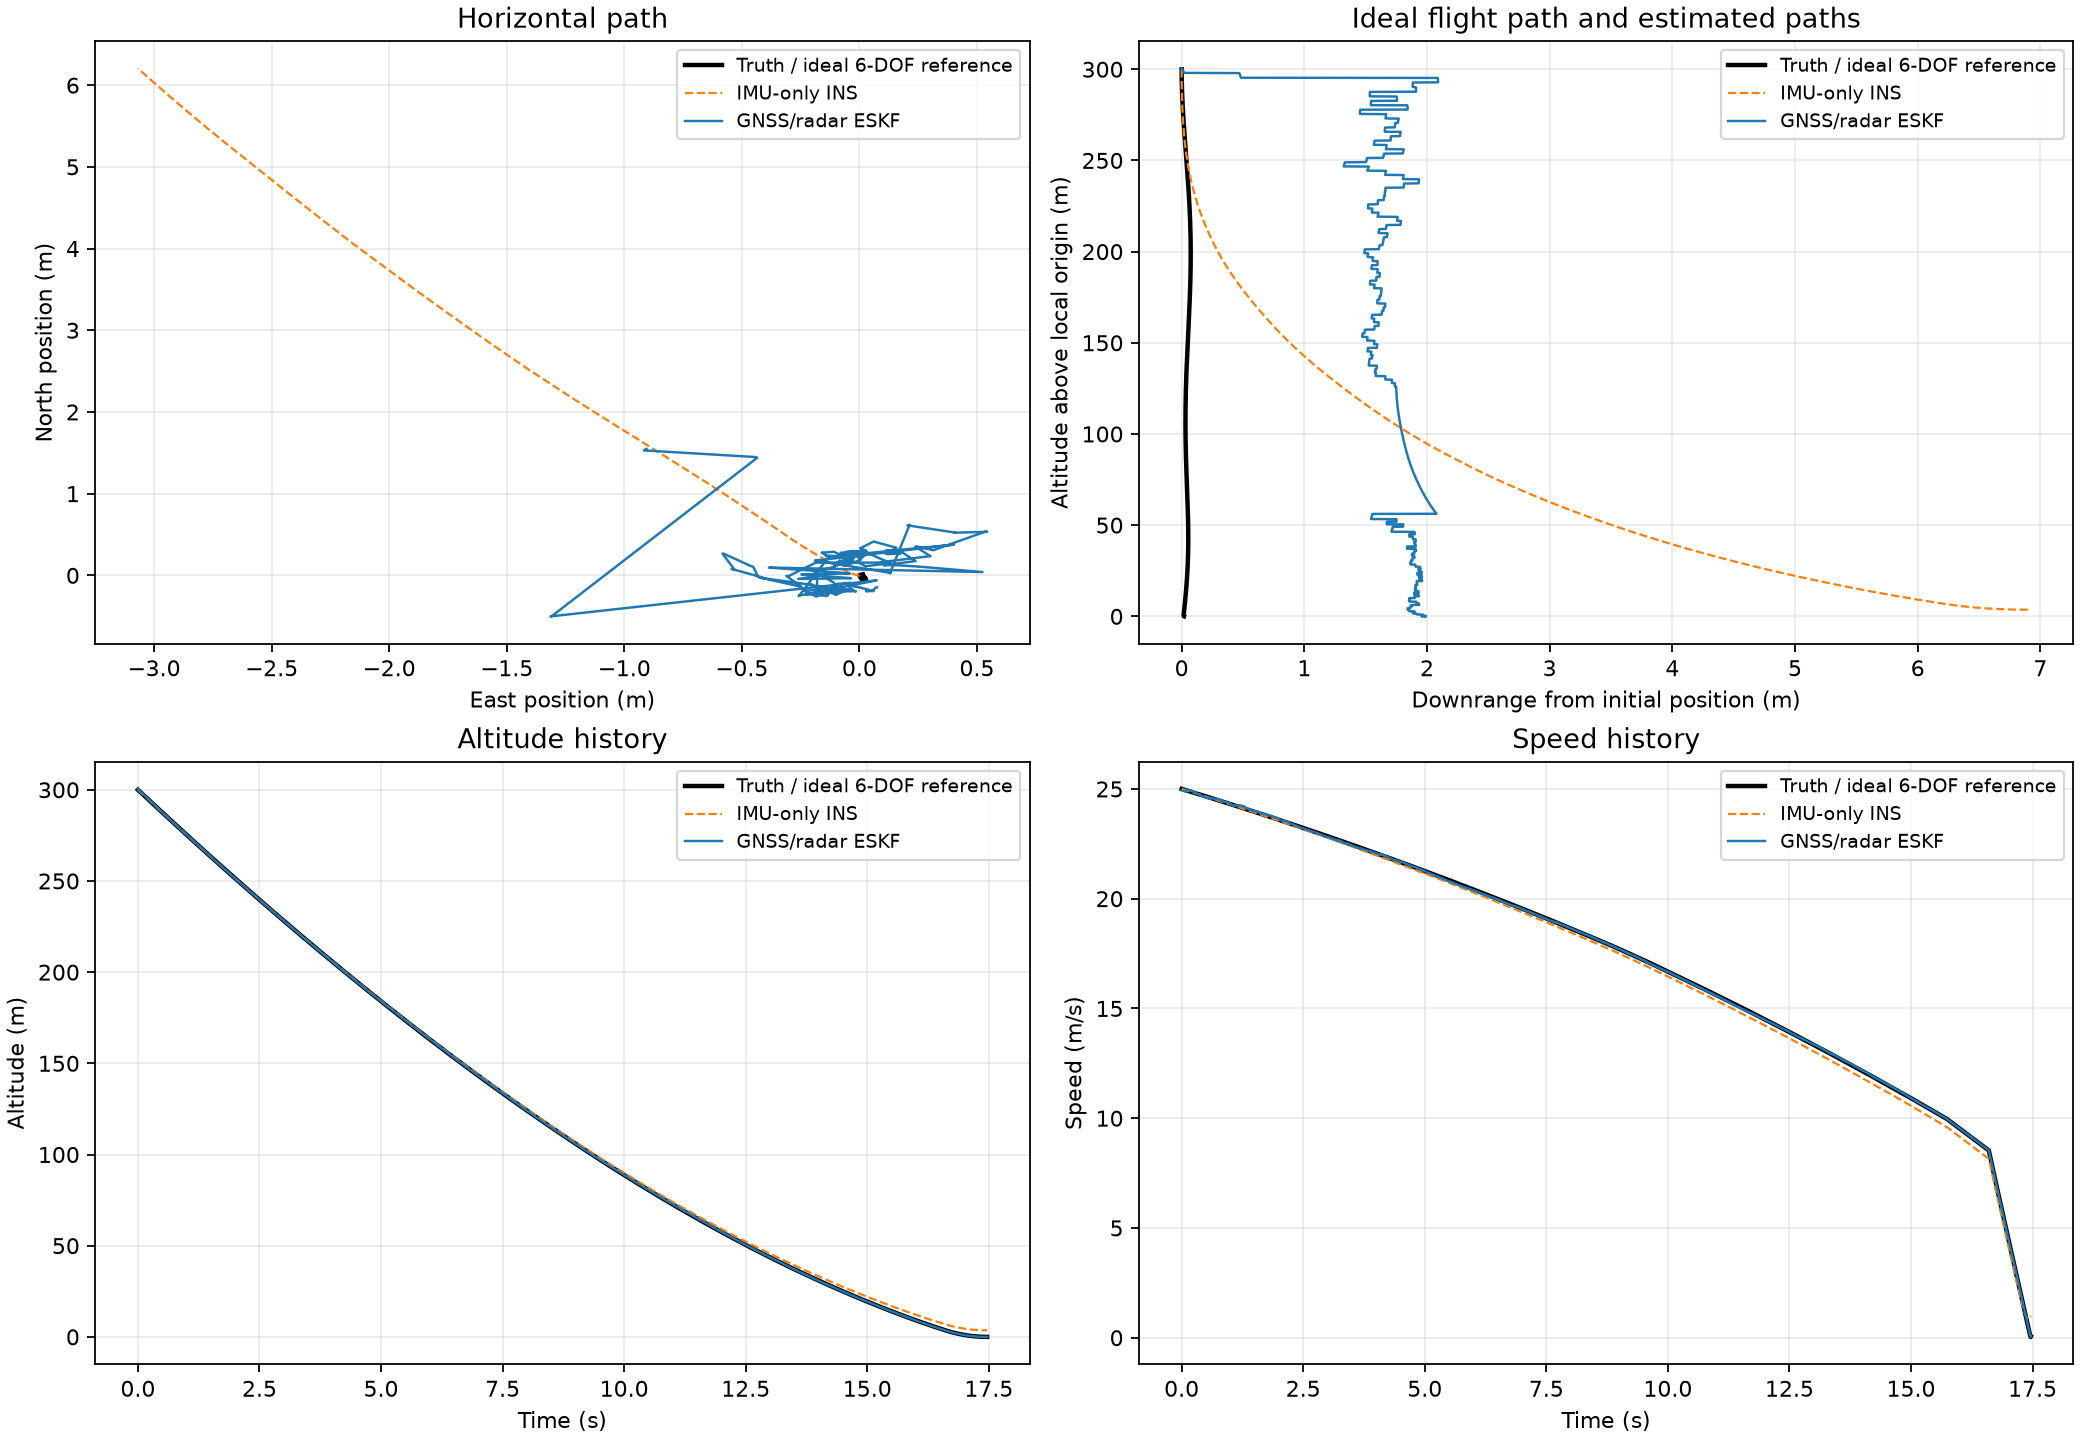
\includegraphics[width=0.97\textwidth]{images/navigation/flight_path_comparison.png}
  \caption{Truth flight path and simulated INS-only and GNSS/radar ESKF estimates.}
\end{figure}

\begin{figure}[p]
  \centering
  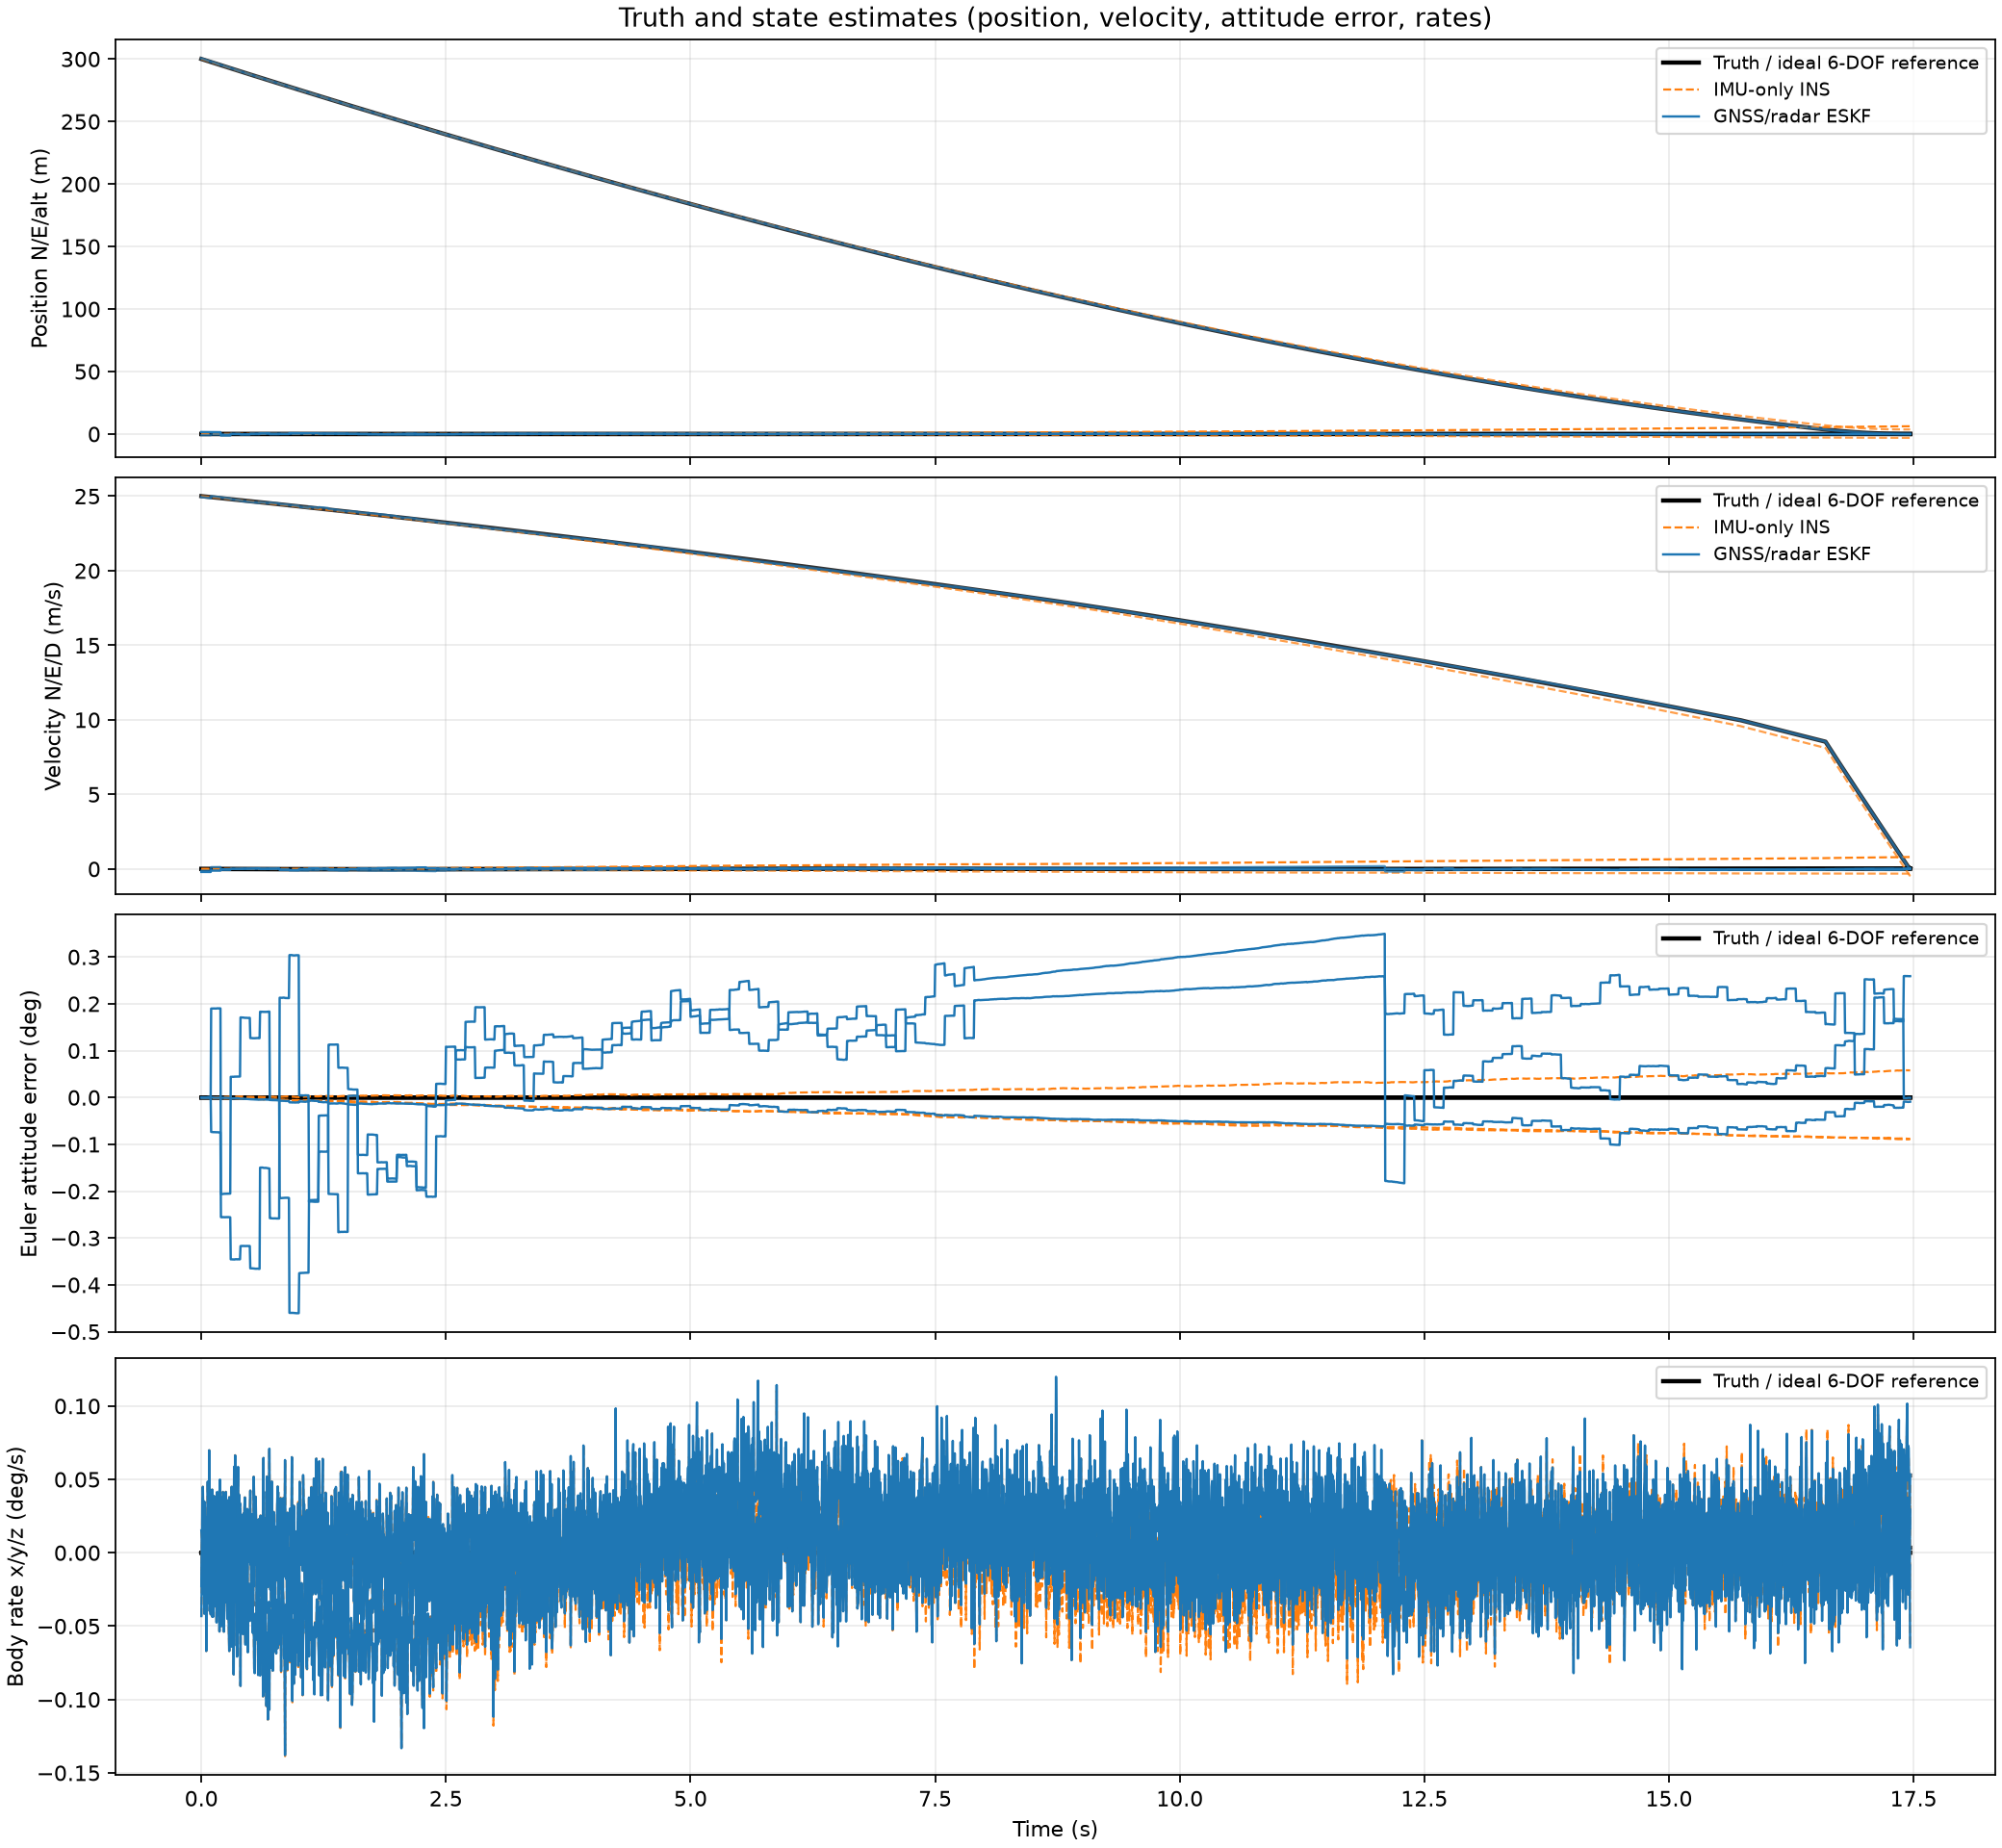
\includegraphics[width=0.97\textwidth]{images/navigation/navigation_state_comparison.png}
  \caption{Truth and estimated position, velocity, relative attitude error, and angular rates.}
\end{figure}

\begin{figure}[p]
  \centering
  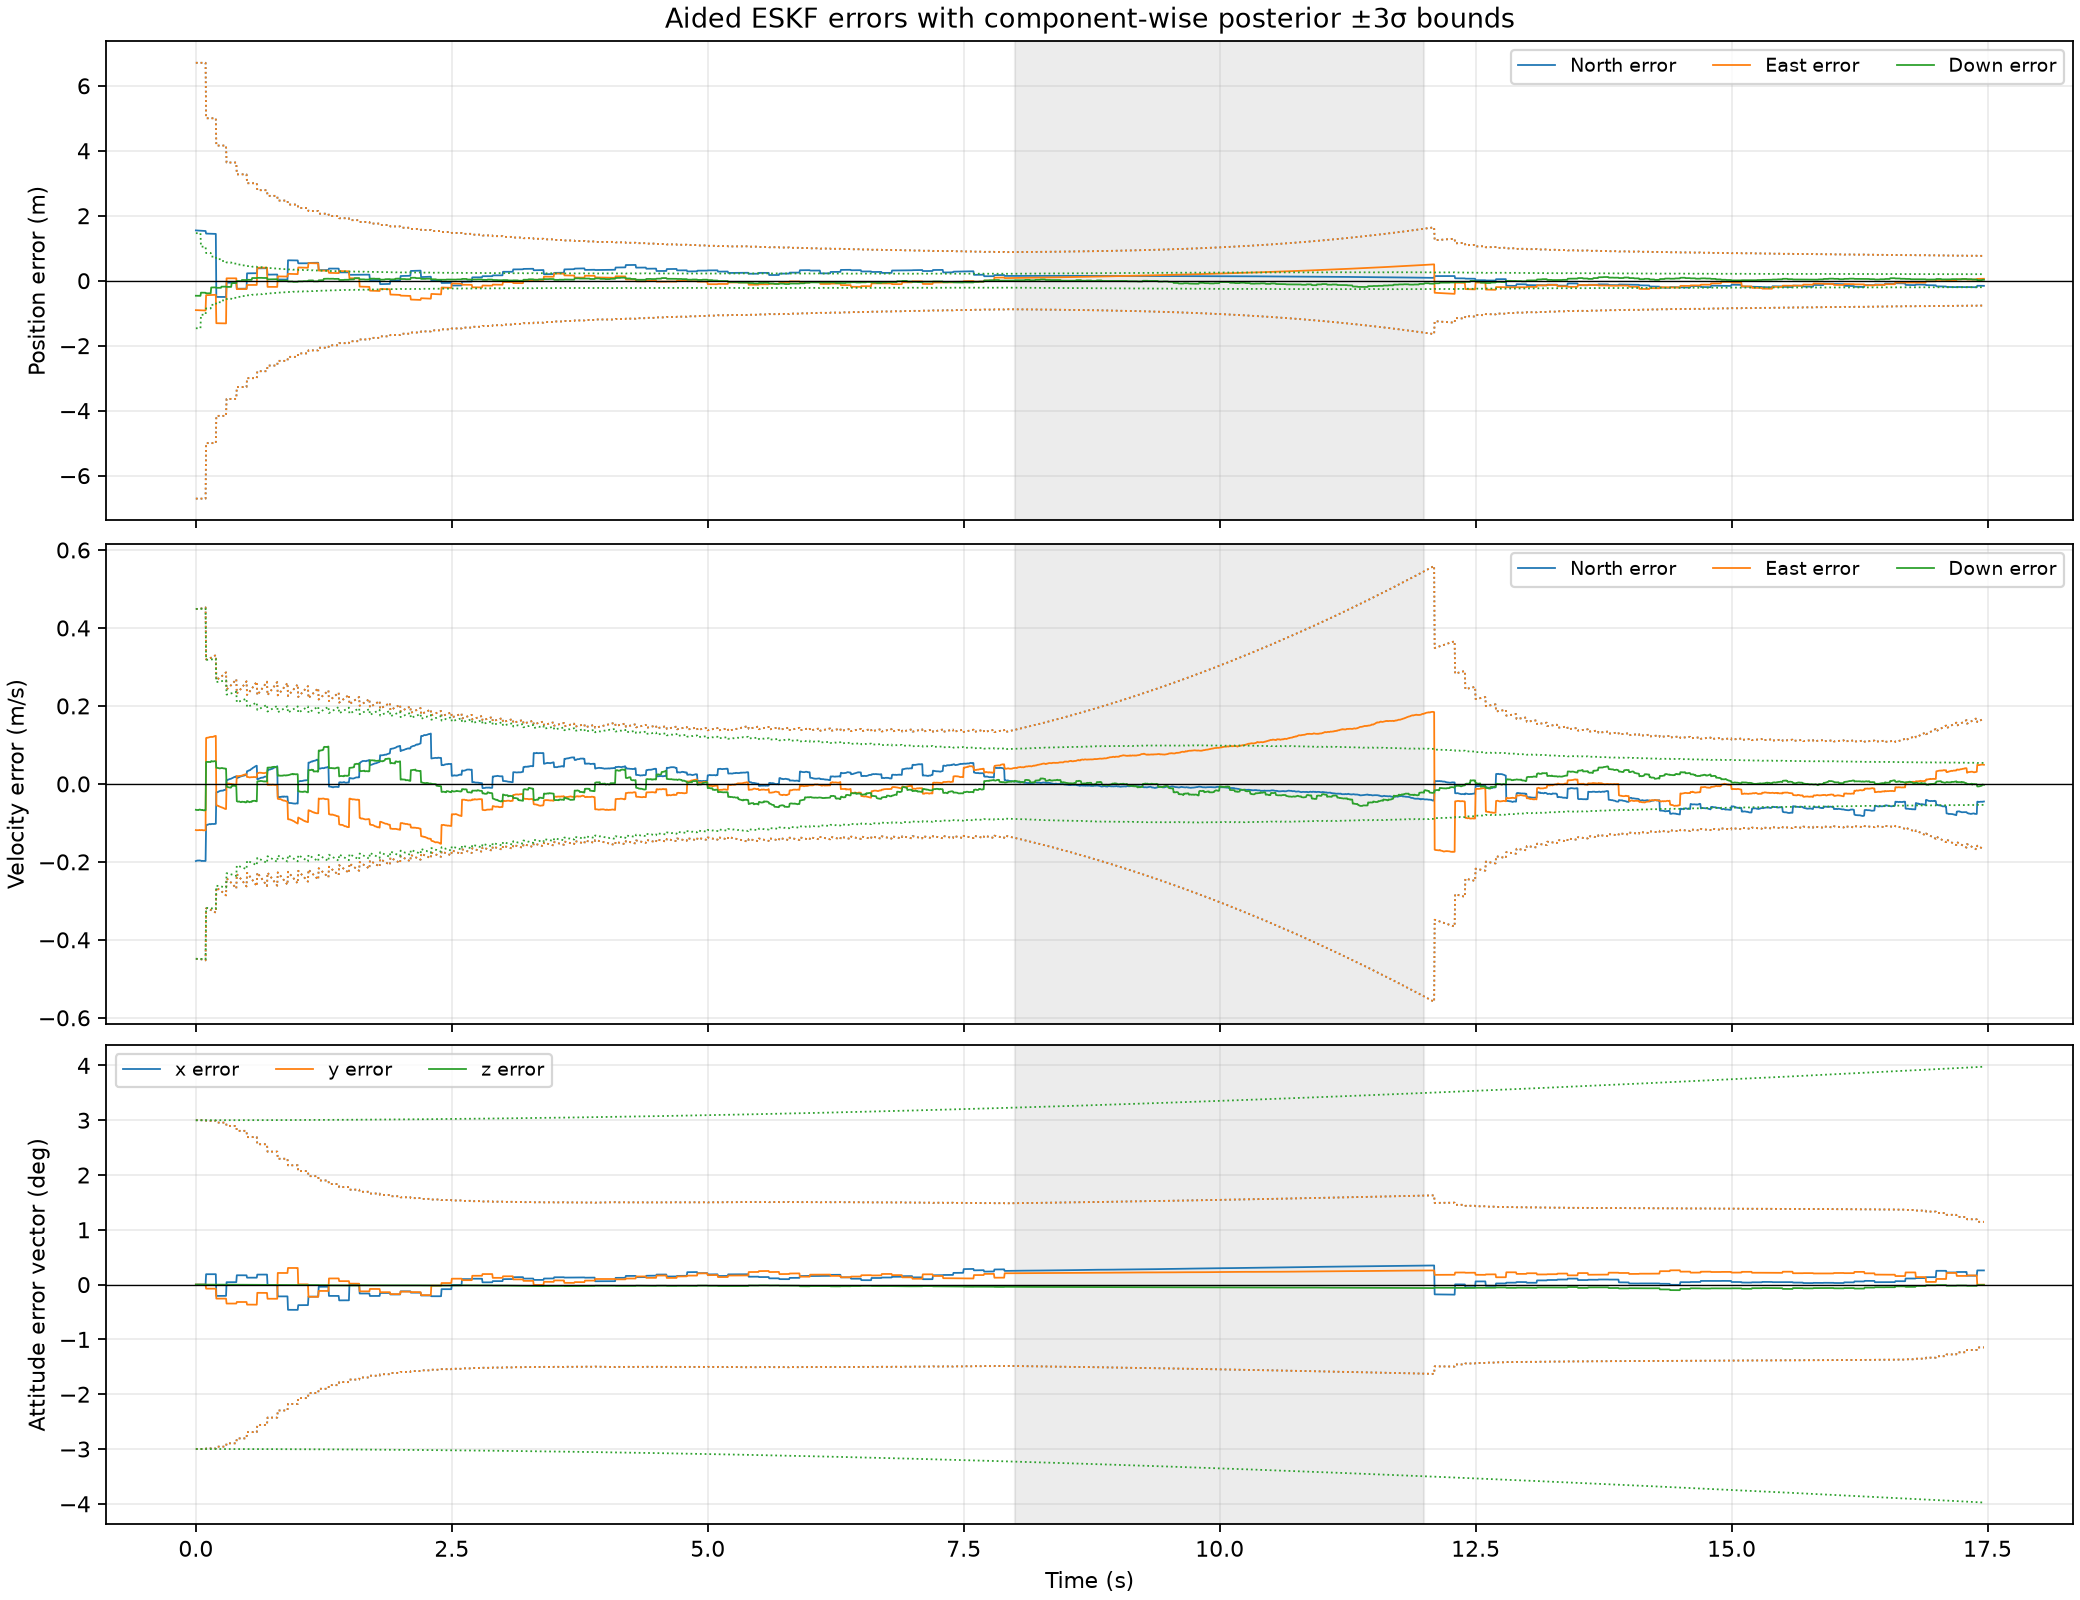
\includegraphics[width=0.97\textwidth]{images/navigation/navigation_consistency.png}
  \caption{Aided ESKF position, velocity, and attitude errors with posterior component-wise $\pm3\sigma$ bounds; shaded region marks the GNSS outage.}
\end{figure}

\begin{figure}[p]
  \centering
  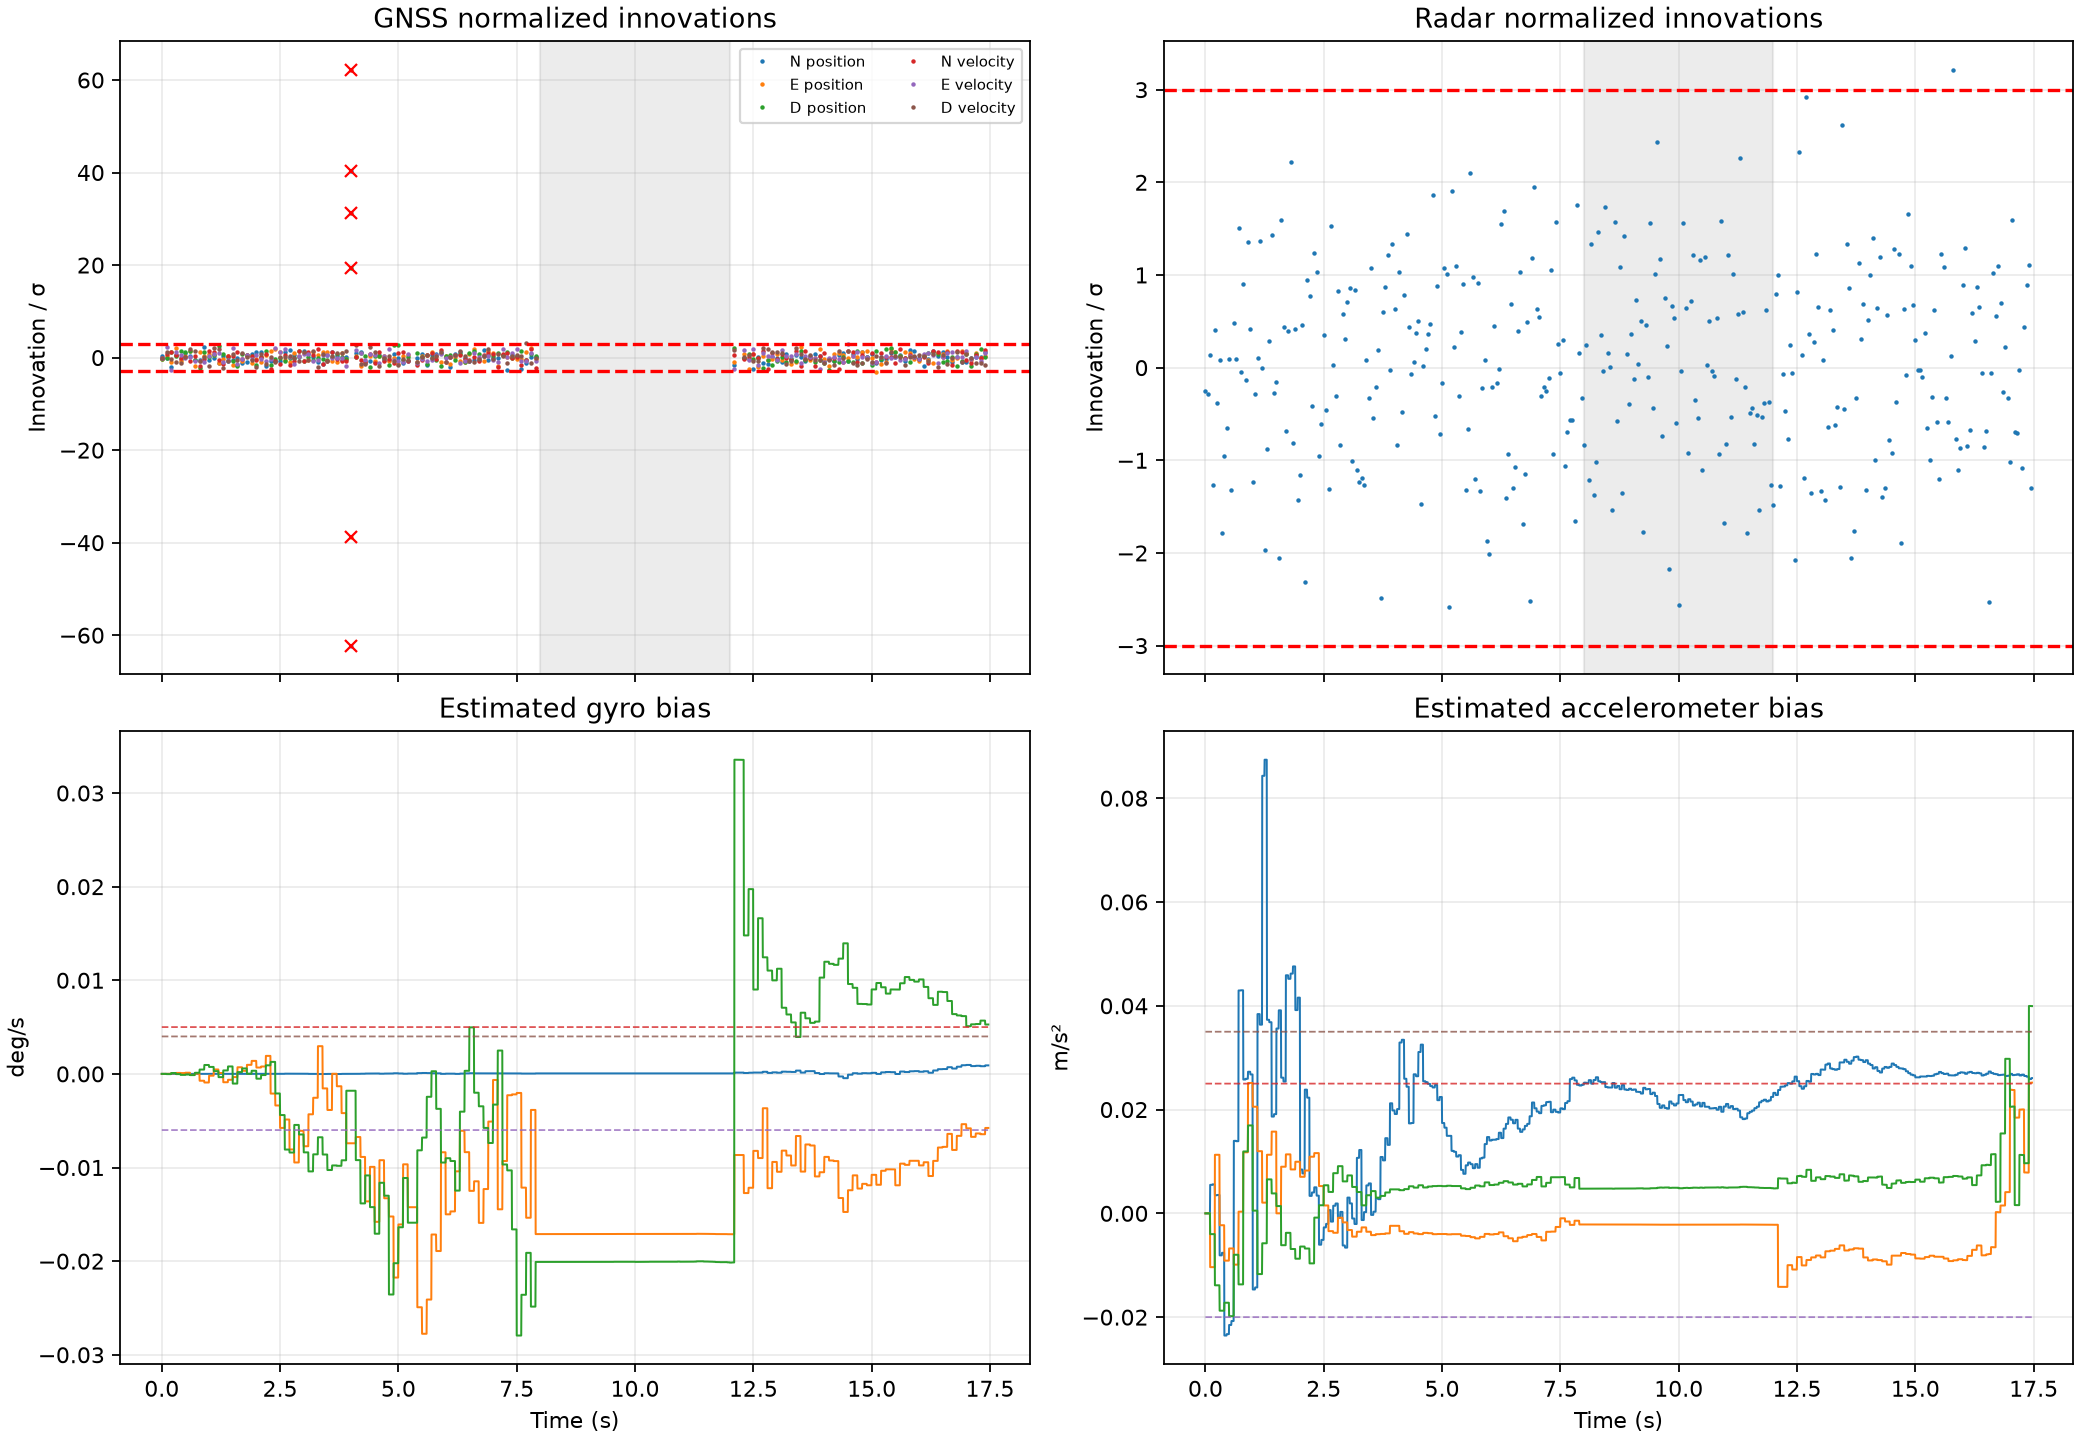
\includegraphics[width=0.97\textwidth]{images/navigation/navigation_innovations_bias.png}
  \caption{Normalized GNSS/radar innovations, gated outlier, and estimated versus injected sensor biases.}
\end{figure}

\section{test}


\end{document}
